\documentclass[degree=doctor, tocarialchapter]{thuthesis}
% 选项
%   degree=[bachelor|master|doctor|postdoctor], % 必选,学位类型
%   secret,                % 可选(默认:关闭),是否有密级
%   tocarialchapter,       % 可选(默认:关闭),章目录中使用黑体(这项表示同时打开下面两项)
%   tocarialchapterentry,  % 可选(默认:关闭),单独控制章标题在目录中使用黑体
%   tocarialchapterpage,   % 可选(默认:关闭),单独控制章页码在目录中使用黑体
%   pifootnote,            % 可选(默认:关闭),页脚编号采用 pifont 字体符号,建议打开

% 所有其它可能用到的包都统一放到这里了,可以根据自己的实际添加或者删除。
\usepackage{thuthesis}

% \usepackage{amsmath}
% \usepackage{amstext}
% \usepackage{amsfonts}
% \usepackage{amssymb}
\usepackage{mathtools}
\usepackage{mathdots}
\usepackage{subcaption}
% \usepackage{arydshln}
\usepackage{dashrule}
\usepackage{mathrsfs}


% 定义所有的图片文件在 figures 子目录下
\graphicspath{{figures/}}

% 可以在这里修改配置文件中的定义。导言区可以使用中文。
% \def\myname{薛瑞尼}

\newcommand{\vect}{\boldsymbol}
\newcommand{\vecr}{\mathbf}
\newcommand{\ii}{\mathrm{i}}

\begin{document}

%%% 封面部分
\frontmatter
% \thusetup{
  %******************************
  % 注意:
  %   1. 配置里面不要出现空行
  %   2. 不需要的配置信息可以删除
  %******************************
  %
  %=====
  % 秘级
  %=====
  secretlevel={秘密},
  secretyear={10},
  %
  %=========
  % 中文信息
  %=========
  ctitle={超冷原子光晶格系统的\\拓扑和动力学研究},
  cdegree={理学博士},
  cdepartment={高等研究院},
  cmajor={物理学},
  cauthor={孙宁},
  csupervisor={翟荟教授},
  % cassosupervisor={陈文光教授}, % 副指导老师
  % ccosupervisor={某某某教授}, % 联合指导老师
  % 日期自动使用当前时间,若需指定按如下方式修改:
  % cdate={超新星纪元},
  %
  % 博士后专有部分
  cfirstdiscipline={物理学},
  cseconddiscipline={系统结构},
  postdoctordate={2009年7月——2011年7月},
  id={编号}, % 可以留空: id={},
  udc={UDC}, % 可以留空
  catalognumber={分类号}, % 可以留空
  %
  %=========
  % 英文信息
  %=========
  etitle={Topology and Dynamics of Ultracold Atoms in Optical Lattices},
  % 这块比较复杂,需要分情况讨论:
  % 1. 学术型硕士
  %    edegree:必须为Master of Arts或Master of Science(注意大小写)
  %             “哲学、文学、历史学、法学、教育学、艺术学门类,公共管理学科
  %              填写Master of Arts,其它填写Master of Science”
  %    emajor:“获得一级学科授权的学科填写一级学科名称,其它填写二级学科名称”
  % 2. 专业型硕士
  %    edegree:“填写专业学位英文名称全称”
  %    emajor:“工程硕士填写工程领域,其它专业学位不填写此项”
  % 3. 学术型博士
  %    edegree:Doctor of Philosophy(注意大小写)
  %    emajor:“获得一级学科授权的学科填写一级学科名称,其它填写二级学科名称”
  % 4. 专业型博士
  %    edegree:“填写专业学位英文名称全称”
  %    emajor:不填写此项
  edegree={Doctor of Philosophy},
  emajor={Physics},
  eauthor={Ning Sun},
  esupervisor={Professor Hui Zhai},
  % eassosupervisor={Chen Wenguang},
  % 日期自动生成,若需指定按如下方式修改:
  % edate={December, 2005}
  %
  % 关键词用“英文逗号”分割
  ckeywords={冷原子, 光晶格, 拓扑, 动力学, 机器学习},
  ekeywords={cold atom, optical lattice, topological matter, dynamics, machine learning}
}

% 定义中英文摘要和关键字
\begin{cabstract}
% 超冷原子物理对于进行凝聚态多体系统的量子模拟、量子计算与量子信息、量子精密调控测量等方面的研究来说具有重要价值,这其中,超冷原子光晶格体系又是进行量子多体研究的重要平台。自2002年人类首次报告在超冷原子光晶格体系中观测到 Mott-超流相变,超冷原子光晶格体系在过去的十几年里受到了理论和实验方面的广泛研究。
% 近年来,得益于调控技术与探测手段方面的进步,人们可以利用光晶格超冷原子气体系统进行更丰富的研究。例如,过去十年里量子气体显微镜的发展,使得人们能够对强相互作用体系的演化进行单原子层面的深入研究,在态的制备等方面也具有更大自由度,可以研究周期含时驱动与动力学淬灭的过程。
超冷原子光晶格系统是进行量子多体物理研究的重要平台,在过去十多年里,这个领域有很多重要进展。调控手段与探测技术的进步使人们可以利用光晶格来进行越来越丰富的研究,例如,近年来量子气体显微镜的发展,使人们能够对一些强相互作用体系进行单格点分辨、时间分辨的测量,在态的制备方面也具有更大的自由度。此外,光晶格体系还可以用来进行周期含时驱动与动力学淬灭等过程的研究。

对超冷原子光晶格体系的理论研究是作者博士期间的主要研究方向,研究重点是其拓扑和动力学性质。本文围绕这两方面介绍了作者博士期间的主要工作。

在拓扑方面:
1)作者和合作者们研究了光晶格中的拓扑电子输运问题,提出了 Creutz 梯上的拓扑电子泵模型,给出了该模型完整的拓扑相图,并发现了模型中存在以偶数为内禀输运单位的绝热拓扑输运路径;
2)作者和合作者们利用深度学习方法研究了拓扑物态的机器学习问题,对机器进行一维 AIII 类 和 二维 A 类的拓扑物态的识别训练,使之取得了超过90\%的精度,且结果具有推广性,能够以较高精度预言未见过的类别;
3)作者为人们常用到的二维材料的陈数算法%\cite{chern2005}
开发了专门的程序包,并证明了该算法的有效性与量子化、规范不变等性质(见附录)。

在含时动力学方面:
1)作者和合作者们证明了一类有 Hubbard 相互作用的体系中受单粒子对称性保护的动力学对称性,该定理能够将几个截然不同的实验现象
%\cite{hubbard-expan-2010,hubbard-expan-2012,mbl1d,twobody-2017}
联系在一起;作者和合作者们用严格对角化的方法对三类例子进行了数值检验;
2)作者和合作者们证明了在二分 Fermi Hubbard 模型中电荷和自旋输运方面存在精确关系;
3)作者和合作者们对周期含时驱动的 Floquet 系统进行了研究,并重点研究了
在近共振高频驱动的框架下的正方晶格 Fermi Hubbard 模型,利用标准路径积分平均场的方法,计算出了完整的平均场相图,并发现了在小的有效相互作用区域存在的铁磁相和相分离;这种铁磁相的出现完全是由近共振的高频驱动以及由其引起的关联隧穿效应所引发,有别于凝聚态中周知的 Stoner 机制。
\end{cabstract}

% 如果习惯关键字跟在摘要文字后面,可以用直接命令来设置,如下:
% ckeywords={冷原子, 光晶格, 拓扑, 动力学, 周期驱动,机器学习},

\begin{eabstract}
Ultracold Atoms are valuable platform for quantum many-body physics. Among all ultracold atom systems, the optical lattices are especially precious. Since the observation of Mott-SF transition in 2002, the study has been getting richer and richer both theoretically and experimentally. Recently, it profits even more from the improvement of detection and manipulation techniques. For example, the development of quantum gas microscope enables one to study quantum many-body system in a more precise way. It also offers more degrees of freedom in preparing states, which can be utilized in the study of quench dynamics and periodic driven systems.

As a doctoral student, the author has been spending a lot of time on the study of the optical lattice systems, focusing on the topology and dynamics. In this thesis, the work on these two aspects are discussed in detail. 

In the topological aspect, the author and collaborators:
1) propose the generalized Creutz model for topological charge pumping, with the complete topological phase diagram given, and a novel type charge pump being discovered that only even units of particles can be transported in one cycle;
2) study the machine learning topological matter problems using deep neural network to classify topological phases in 1D AIII class and 2D A class. The network achieves an over-90\% test accuracy with a generalizing ability to recognize phases that has not been fed in training.
% 3) For the common algorithm for calculating Chern number, the author develop special libraries of codes. The author also proves some theorems and properties demonstrating it's efficiency and powerfulness. (See appendix)

In the dynamics aspect, the author and collaborators:
1) propose a symmetry protected dynamical symmetry in a series of Hubbard models, providing a unified way of understanding to several quite different experiments recently in cold atom community; carry out numerics examination using exact diagonalization for three classes of examples; 
2) prove some exact relations in the charge transport and spin transport in bipartite Fermi Hubbard systems;
3) study the periodic driving Fermi Hubbard lattices, with a deep focus on the nearly resonant driving; use the standard path integral approach to establish a mean-field treatment, and numerically compute the phase diagram. There is a novel ferromagnetism (FM) phase emergent in small effective interaction regime, induced by the correlated tunneling effect generated by the nearly resonant periodic driving. This differs from the well-known Stoner mechanism attributing the FM to large interaction. 
\end{eabstract}

% ekeywords={cold atom, optical lattice, topological matter, dynamics, Floquet, machine learning}

\thusetup{
  %******************************
  % 注意:
  %   1. 配置里面不要出现空行
  %   2. 不需要的配置信息可以删除
  %******************************
  %
  %=====
  % 秘级
  %=====
  secretlevel={秘密},
  secretyear={10},
  %
  %=========
  % 中文信息
  %=========
  ctitle={超冷原子光晶格系统的\\拓扑和动力学研究},
  cdegree={理学博士},
  cdepartment={高等研究院},
  cmajor={物理学},
  cauthor={孙宁},
  csupervisor={翟荟教授},
  % cassosupervisor={陈文光教授}, % 副指导老师
  % ccosupervisor={某某某教授}, % 联合指导老师
  % 日期自动使用当前时间,若需指定按如下方式修改:
  % cdate={超新星纪元},
  %
  % 博士后专有部分
  cfirstdiscipline={物理学},
  cseconddiscipline={系统结构},
  postdoctordate={2009年7月——2011年7月},
  id={编号}, % 可以留空: id={},
  udc={UDC}, % 可以留空
  catalognumber={分类号}, % 可以留空
  %
  %=========
  % 英文信息
  %=========
  etitle={Topology and Dynamics of Ultracold Atoms in Optical Lattices},
  % 这块比较复杂,需要分情况讨论:
  % 1. 学术型硕士
  %    edegree:必须为Master of Arts或Master of Science(注意大小写)
  %             “哲学、文学、历史学、法学、教育学、艺术学门类,公共管理学科
  %              填写Master of Arts,其它填写Master of Science”
  %    emajor:“获得一级学科授权的学科填写一级学科名称,其它填写二级学科名称”
  % 2. 专业型硕士
  %    edegree:“填写专业学位英文名称全称”
  %    emajor:“工程硕士填写工程领域,其它专业学位不填写此项”
  % 3. 学术型博士
  %    edegree:Doctor of Philosophy(注意大小写)
  %    emajor:“获得一级学科授权的学科填写一级学科名称,其它填写二级学科名称”
  % 4. 专业型博士
  %    edegree:“填写专业学位英文名称全称”
  %    emajor:不填写此项
  edegree={Doctor of Philosophy},
  emajor={Physics},
  eauthor={Ning Sun},
  esupervisor={Professor Hui Zhai},
  % eassosupervisor={Chen Wenguang},
  % 日期自动生成,若需指定按如下方式修改:
  % edate={December, 2005}
  %
  % 关键词用“英文逗号”分割
  ckeywords={冷原子, 光晶格, 拓扑, 动力学, 机器学习},
  ekeywords={cold atom, optical lattice, topological matter, dynamics, machine learning}
}

% 定义中英文摘要和关键字
\begin{cabstract}
% 超冷原子物理对于进行凝聚态多体系统的量子模拟、量子计算与量子信息、量子精密调控测量等方面的研究来说具有重要价值,这其中,超冷原子光晶格体系又是进行量子多体研究的重要平台。自2002年人类首次报告在超冷原子光晶格体系中观测到 Mott-超流相变,超冷原子光晶格体系在过去的十几年里受到了理论和实验方面的广泛研究。
% 近年来,得益于调控技术与探测手段方面的进步,人们可以利用光晶格超冷原子气体系统进行更丰富的研究。例如,过去十年里量子气体显微镜的发展,使得人们能够对强相互作用体系的演化进行单原子层面的深入研究,在态的制备等方面也具有更大自由度,可以研究周期含时驱动与动力学淬灭的过程。
超冷原子光晶格系统是进行量子多体物理研究的重要平台,在过去十多年里,这个领域有很多重要进展。调控手段与探测技术的进步使人们可以利用光晶格来进行越来越丰富的研究,例如,近年来量子气体显微镜的发展,使人们能够对一些强相互作用体系进行单格点分辨、时间分辨的测量,在态的制备方面也具有更大的自由度。此外,光晶格体系还可以用来进行周期含时驱动与动力学淬灭等过程的研究。

对超冷原子光晶格体系的理论研究是作者博士期间的主要研究方向,研究重点是其拓扑和动力学性质。本文围绕这两方面介绍了作者博士期间的主要工作。

在拓扑方面:
1)作者和合作者们研究了光晶格中的拓扑电子输运问题,提出了 Creutz 梯上的拓扑电子泵模型,给出了该模型完整的拓扑相图,并发现了模型中存在以偶数为内禀输运单位的绝热拓扑输运路径;
2)作者和合作者们利用深度学习方法研究了拓扑物态的机器学习问题,对机器进行一维 AIII 类 和 二维 A 类的拓扑物态的识别训练,使之取得了超过90\%的精度,且结果具有推广性,能够以较高精度预言未见过的类别;
3)作者为人们常用到的二维材料的陈数算法%\cite{chern2005}
开发了专门的程序包,并证明了该算法的有效性与量子化、规范不变等性质(见附录)。

在含时动力学方面:
1)作者和合作者们证明了一类有 Hubbard 相互作用的体系中受单粒子对称性保护的动力学对称性,该定理能够将几个截然不同的实验现象
%\cite{hubbard-expan-2010,hubbard-expan-2012,mbl1d,twobody-2017}
联系在一起;作者和合作者们用严格对角化的方法对三类例子进行了数值检验;
2)作者和合作者们证明了在二分 Fermi Hubbard 模型中电荷和自旋输运方面存在精确关系;
3)作者和合作者们对周期含时驱动的 Floquet 系统进行了研究,并重点研究了
在近共振高频驱动的框架下的正方晶格 Fermi Hubbard 模型,利用标准路径积分平均场的方法,计算出了完整的平均场相图,并发现了在小的有效相互作用区域存在的铁磁相和相分离;这种铁磁相的出现完全是由近共振的高频驱动以及由其引起的关联隧穿效应所引发,有别于凝聚态中周知的 Stoner 机制。
\end{cabstract}

% 如果习惯关键字跟在摘要文字后面,可以用直接命令来设置,如下:
% ckeywords={冷原子, 光晶格, 拓扑, 动力学, 周期驱动,机器学习},

\begin{eabstract}
Ultracold Atoms are valuable platform for quantum many-body physics. Among all ultracold atom systems, the optical lattices are especially precious. Since the observation of Mott-SF transition in 2002, the study has been getting richer and richer both theoretically and experimentally. Recently, it profits even more from the improvement of detection and manipulation techniques. For example, the development of quantum gas microscope enables one to study quantum many-body system in a more precise way. It also offers more degrees of freedom in preparing states, which can be utilized in the study of quench dynamics and periodic driven systems.

As a doctoral student, the author has been spending a lot of time on the study of the optical lattice systems, focusing on the topology and dynamics. In this thesis, the work on these two aspects are discussed in detail. 

In the topological aspect, the author and collaborators:
1) propose the generalized Creutz model for topological charge pumping, with the complete topological phase diagram given, and a novel type charge pump being discovered that only even units of particles can be transported in one cycle;
2) study the machine learning topological matter problems using deep neural network to classify topological phases in 1D AIII class and 2D A class. The network achieves an over-90\% test accuracy with a generalizing ability to recognize phases that has not been fed in training.
% 3) For the common algorithm for calculating Chern number, the author develop special libraries of codes. The author also proves some theorems and properties demonstrating it's efficiency and powerfulness. (See appendix)

In the dynamics aspect, the author and collaborators:
1) propose a symmetry protected dynamical symmetry in a series of Hubbard models, providing a unified way of understanding to several quite different experiments recently in cold atom community; carry out numerics examination using exact diagonalization for three classes of examples; 
2) prove some exact relations in the charge transport and spin transport in bipartite Fermi Hubbard systems;
3) study the periodic driving Fermi Hubbard lattices, with a deep focus on the nearly resonant driving; use the standard path integral approach to establish a mean-field treatment, and numerically compute the phase diagram. There is a novel ferromagnetism (FM) phase emergent in small effective interaction regime, induced by the correlated tunneling effect generated by the nearly resonant periodic driving. This differs from the well-known Stoner mechanism attributing the FM to large interaction. 
\end{eabstract}

% ekeywords={cold atom, optical lattice, topological matter, dynamics, Floquet, machine learning}

% 如果使用授权说明扫描页,将可选参数中指定为扫描得到的 PDF 文件名,例如:
% \makecover[scan-auth.pdf]
\makecover

%% 目录
\tableofcontents

%% 符号对照表
\begin{denotation}[3cm]
\item[$\hat{H}$] 哈密顿量
\item[$\hat{H}(t)$] 有含时依赖的哈密顿量
\item[$\hat{H}_F$] Floquet 哈密顿量
\item[$\hat{H}_{\text{eff}}$] 有效静态哈密顿量
\item[$\hat{H}(\vect{k})$] 动量空间哈密顿量
\item[$\hat{U}(T)$] 一个周期的幺正演化算符
\item[$J$] 最近邻跃迁矩阵元
\item[$U$] Hubbard 相互作用强度
\item[$\hat{c}^{\dagger}_{i\sigma}$] 格点 $i$ 上自旋为 $\sigma$ 的费米子湮灭算符
\item[$\hat{c}^{\dagger}_{i\sigma}$] 格点 $i$ 上自旋为 $\sigma$ 的费米子产生算符
\item[$\hat{n}_{i\sigma}$] 格点 $i$ 上自旋为 $\sigma$ 的粒子数
\item[$\bar\psi, \psi$] 费米子场算符
\item[$\mathcal{L}$] 拉式量
\item[$\mathcal{Z}$] 配分函数
\item[$\rho$] 混合系综密度矩阵
\item[$t$] 作为变量的时间,或作为模型参数的最近邻跃迁系数,依赖于上下文
\item[$\vect{k}$] 动量
\item[$\vect{q}$] 准动量
\item[$T$] 含时依赖周期或体系温度,依赖于上下文
\item[$\omega$] 驱动频率
\item[$A$] 驱动振幅
\item[$T^2$] Torus 结构,即二维参数空间且两个方向均为周期性边界条件的几何结构
\item[$S^2$] 球面
\item[$F_{\mu\nu}$] 二维 Berry 曲率
\item[$A_{\mu}$] Berry 连接
\end{denotation}



% % 也可以使用 nomencl 宏包:

% \printnomenclature[3cm]

% \nomenclature{HPC}{高性能计算 (High Performance Computing)}
% \nomenclature{cluster}{集群}
% \nomenclature{Itanium}{安腾}
% \nomenclature{SMP}{对称多处理}
% \nomenclature{API}{应用程序编程接口}
% \nomenclature{PI}{聚酰亚胺}
% \nomenclature{MPI}{聚酰亚胺模型化合物,N-苯基邻苯酰亚胺}
% \nomenclature{PBI}{聚苯并咪唑}
% \nomenclature{MPBI}{聚苯并咪唑模型化合物,N-苯基苯并咪唑}
% \nomenclature{PY}{聚吡咙}
% \nomenclature{PMDA-BDA}{均苯四酸二酐与联苯四胺合成的聚吡咙薄膜}
% \nomenclature{$\Delta G$}{活化自由能 (Activation Free Energy)}
% \nomenclature{$\chi$}{传输系数 (Transmission Coefficient)}
% \nomenclature{$E$}{能量}
% \nomenclature{$m$}{质量}
% \nomenclature{$c$}{光速}
% \nomenclature{$P$}{概率}
% \nomenclature{$T$}{时间}
% \nomenclature{$v$}{速度}



%%% 正文部分
\mainmatter
% \include{data/chap01}
% \include{data/chap02}
\chapter{超冷原子光晶格系统简介}
\label{cha:intro}

1995年,人类首次在稀薄的冷原子气体中直接观测到碱金属原子的玻色爱因斯坦凝聚\cite{bec1995a,bec1995b}。自那时起,冷原子物理作为一个新兴的研究领域,在之后的20多年时间里蓬勃发展。人们对稀薄的超冷原子气体系统展开研究,取得了许多重要的成果,这些成果揭示了冷原子物理在进行凝聚态多体系统的量子模拟、量子计算与量子信息、量子体系含时动力学研究、量子光学、以及量子器件与精密测量等方面研究的重要价值\cite{bloch2012}。例如,通过激光驻波作用在超冷原子气体上,形成周期性势场(光晶格),可以用来模拟凝聚态物理中的 Hubbard 模型等许多模型在不同参数条件下的行为。冷原子物理所做的量子模拟并非简单的复制和模仿,而是创造性的模拟。一方面,经过与现有最前沿量子蒙特卡洛等方法的结果进行校准,利用光晶格中的超冷原子系统实现了对具体模型的高精度的仿真;另一方面,经过校准后的光晶格模拟器又可以模拟更极端参数下的行为,和更大的体系,而经典计算机对很大的体系缺乏有效的数值模拟算法,从而实现量子模拟对经典计算机的超越\cite{feynman1982,qsgoals2012}。近年来,得益于调控手段与探测技术的双方面的进步,人们可以对强相互作用体系的演化进行单原子层面的深入研究,甚至研究一些传统凝聚态很难实现的体系,如含时驱动体系和非平衡态过程。超冷原子光晶格体系的研究价值逐渐彰显。对这种光晶格中超冷原子气体的理论研究是作者博士期间的主要研究方向,研究重点是其拓扑和含时动力学性质。下面将做具体介绍。


\section{超冷原子光晶格系统与量子模拟}

在凝聚态物理中,固体中的电子运动在带电离子实规则排列形成的周期性晶格势场中。对于这样的周期性结构,冷原子物理中可以用光晶格来进行模拟。对一团中性超冷原子气体,利用激光驻波作用其上可以形成周期性的光晶格势场,用来模拟固体材料中离子实形成的周期性势场,而超冷原子气体在势场中的运动行为则用来模拟固体中的电子的运动行为。通过将几个方向的激光进行不同角度的叠加,可以产生出正方晶格、三角晶格、六角晶格、蜂巢晶格、甚至 Kagome 晶格等,可以用来模拟凝聚态中许多不同的模型,包括带阻错的模型。光晶格中原子和原子间的相互作用一方面可以通过 Feshbach 共振的技术来进行调节\cite{feshbach2010},通过直接调节原子间的散射长度来实现格点上原子间的相互作用强度的调节。另一方面,也可以通过调节光晶格的势阱深度来调节原子间的相互作用与格点间跃迁动能之间的相对大小($U/J$)\cite{bloch2012}。当光势阱较浅时,晶格格点上的局域化 Wannier 波函数有较宽的展宽,临近格点的 Wannier 波函数有较大重合,跃迁矩阵元较大,相应的,$U/J$较小;而当势阱深度很深时,晶格格点上的 Wannier 波函数被更多的局域化在自己的格点上,与其他格点上的 Wannier 波函数重叠很小,相应的,跃迁矩阵元很小,$U/J$则很大,体系的能带(与相互作用能量相比)趋近于平带。通过类似的方式,人们实现了三维光晶格中超冷原子气体从超流到 Mott 绝缘体的量子相变\cite{mott-sf-2002},以及许多不同的凝聚态体系的量子模拟。

过去,在利用稀薄的超冷原子气体进行量子多体强关联现象的研究方面有过许多的理论和实验的进展\cite{bloch2008}。这些研究所关注的问题超出一般的弱的相互作用体系的描述,而是更集中于原子间强的相互作用所引起的效应,例如光晶格中的 Mott-Hubbard 相变,一维和二维体系中的强相互作用气体,以及在快速旋转的准二维气体中的最低朗道能级等。光晶格中的强关联费米气体也是一个重要的研究方向,这样的系统往往可以用来对传统凝聚态中的重要模型进行模拟,如 Hubbard 模型和 Heisenberg 自旋模型。研究这些重要的模型,以及这些体系中的铁磁/反铁磁关联、热力学性质、动力学性质以及输运性质的研究,对于理解传统凝聚态强关联系统的现象,例如分数量子霍尔效应和 高温超导等现象,有着重要帮助\cite{nagaosa}。

近来,冷原子实验在调控与探测光晶格中的中性原子技术方面有许多重大进展。例如,通过调节一系列参数,诸如散射长度、晶格势阱深度、外部禁闭等,人们可以绝热地调节中性原子气体间从很弱的相互作用到很强的相互作用。再如,量子气体显微镜的发展是过去十年中冷原子物理领域的重要进展\cite{microscope1,microscope2,microscope3,microscope4,microscope5,microscope6},一方面,它允许人们对光晶格中的冷原子体系做晶格上的单原子探测,另一方面,它使得人们在态的制备方面有了更大的自由度,可以制备实空间密度算符的本征态(例如电荷密度波态和自旋密度波态)作为初态进行研究。这些进展使得超冷原子光晶格系统对于进行量子多体强关联体系的研究来说更加具有价值。

可以利用超冷原子光晶格系统进行研究的量子多体系统包括\cite{olbook}:

\begin{itemize}

\item 一大类 Hubbard 模型\cite{hubbard-expan-2010,hubbard-expan-2012,microscope5,microscope6,af1,af2,af3,canted,incommensurate,af_long_range,pair_attractive,hidden_af_doped,charge-diffusion,spin-diffusion,floq-hubb-expr-2018,correlated-tunnel-expr-2018-shaking,correlated-tunnel-expr-2018-raman},带有格点上相互作用的单带模型乃至 $t-J$ 模型\cite{olbook},包括费米子的,玻色子的\cite{twobody-2017},带磁通的\cite{twobody-2017},吸引相互作用的\cite{pair_attractive},排斥相互作用的,半填充的\cite{microscope5,microscope6},掺杂的\cite{hidden_af_doped},磁中性的,有磁梯度的\cite{twobody-2017},有关联隧穿效应的\cite{floq-hubb-expr-2018,correlated-tunnel-expr-2018-shaking,correlated-tunnel-expr-2018-raman},等等,以及对其中的短程关联\cite{af1,af2,af3}、(准)长程关联\cite{af_long_range,canted,pair_attractive,hidden_af_doped}、输运性质\cite{charge-diffusion,spin-diffusion}、少体相互作用性质\cite{twobody-2017}等等的研究和测量。

\item 一大类量子霍尔效应(Quantum Hall)同源的物理系统和过程\cite{topo2016zoller,harper1,harper2,zak-expr-2013,chern-expr-2015,ab-expr-2015,wilsonline-expr-2016,haldane-expr-2014,charge-pump-expr-2016-de,charge-pump-expr-2016-jp,4dqhall-expr-2018},拓扑物态,(非交换)几何物理,如各种非平庸的 Berry 相\cite{ab-expr-2015},Zak 相\cite{zak-expr-2013},非阿贝尔 Wilson 路径\cite{wilsonline-expr-2016}等等,以及 Haldane 模型\cite{haldane-expr-2014},Harper-Hofstadter 模型\cite{harper1,harper2},Thouless 拓扑电子泵\cite{charge-pump-expr-2016-de,charge-pump-expr-2016-jp},四维量子霍尔效应\cite{4dqhall-expr-2018},等等。

\item 各种自旋模型\cite{spin-chain-expr-2011},包括 Ising 模型,Heisenberg 模型,XXZ 模型等\cite{olbook}。

\item 无序系统\cite{mbl1d,mbl2d},包括 Anderson 局域化和多体局域化等系统,利用不公度的晶格实现准无序系统的 准一维 Aubry-Andre 模型\cite{mbl1d},二维多体局域化模型\cite{mbl2d}等。

\item 不同维度的物理,包括一维\cite{incommensurate,spin-chain-expr-2011,af2,hidden_af_doped} Luttinger 液体,自旋电荷分离,非公度的自旋波和电荷波激发\cite{incommensurate},二维的短程关联和准长程序\cite{microscope5,microscope6,af1,af3,canted,af_long_range,pair_attractive,twobody-2017}等等。

\end{itemize}

% 等等。

此外,利用超冷原子光晶格体系还可以实现一些传统凝聚态很难实现的物理过程,如周期含时驱动的体系与动力学淬灭过程等。一方面,周期含时驱动的体系给人们 提供了实现一些有效稳态模型的方式,例如通过高频率周期含时驱动所生成的 Floquet-拓扑绝缘体\cite{floq-ti-2011},和前面提到的 Haldane 模型的实现\cite{haldane-expr-2014}与关联隧穿 Hubbard 体系\cite{floq-hubb-expr-2018,correlated-tunnel-expr-2018-shaking};另一方面,与静态系统相比,周期含时驱动本身就会使系统在诸如拓扑性质等内在性质方面有很大区别,例如,对周期驱动体系的拓扑分类与静态系统有着内禀的不同\cite{floq-edgestate-2013-prx}。此外,通过对这些系统的研究,人们可以研究一些传统凝聚态很少研究或很难用实验研究的物理过程,例如非平衡态的问题,还有从单个纯态出发的动力学淬灭的过程,甚至包括本征态热化假说(Eigenstate Themalization Hypothesis)\cite{thermalize-entropy-2016}这样的量子力学基本问题等。




\section{光晶格系统中的拓扑物态}


凝聚态物理中一个重要的主题是对不同的物质的相的刻画与分类。传统的朗道相变理论从对称性出发来描述物质的相和相变,即物质的相由体系的对称性以及态的对称性自发破缺来刻画,态的对称性自发破缺形成物质的序。然而,从上世纪80年代开始,一系列对量子霍尔效应的研究打开了新世界的大门,有一类物态并没有破缺体系的对称性,但却可以定义某种序,这些序决定着体系最基本的一些性质(例如材料的横向电导),而且对于材料的参数变化具有鲁棒性。这样的序可以用某个拓扑不变量来刻画,被称为体系的拓扑数,这类物态被称为拓扑物态。体系的某些基本性质,例如量子化的霍尔电导平台,都由这个拓扑数来刻画。材料的连续的微小的扰动不会改变体系的拓扑数,相应的也不会改变体系的那些基本的性质,只有发生较大变化,使体系经历量子相变(关闭能隙再打开),态的拓扑数才有可能改变。

拓扑物态中有一类拓扑绝缘体在过去十几年中被广泛研究\cite{topo2010hasan}。拓扑绝缘体是指一类电子材料,它们的体材料如同普通的能带绝缘体一样,电子填充价带而导带空置,价带和导带之间有能隙,因此体材料并不导电,但其边界或表面上却局域着导电的边缘态。这种边缘态受材料的拓扑数所保护,对于材料的微小、连续的扰动具有鲁棒性,并且对于体系的微小的无序性具有鲁棒性,不会与其他态发生背散射,这也正是其具有量子化的霍尔电导平台的原因。

拓扑物态所具有的良好性质吸引人们进行了许多理论和实验的研究,包括对拓扑材料的探索。而拓扑绝缘体之能发生于周期性晶格结构,也使得利用超冷原子光晶格系统进行探索成为可能。然而超冷原子系统进行研究的一个问题是,如何模拟电磁规范场。由于光晶格中的中性原子并不带电,并不能通过直接加电场或磁场的方式来使体系产生电磁规范场。对此,人们发展了利用光诱导产生人工规范场\cite{lightgauge2014}的方法来进行研究。通过拉曼光耦合原子不同的内态,可以实现有效的自旋轨道耦合。类似地,通过拉曼光的帮助,利用Aharonov-Bohm 效应(以下简称AB效应)的原理,可以实现晶格方块上的磁通\cite{harper1,harper2}。这样的模型模拟了凝聚态物理中著名的 Hofstadter-Harper 模型\cite{topobook},在某些系统参数区间内,这样的模型具有非平庸的拓扑态\cite{topobook}。此外,人们还可以对光晶格系统进行周期性含时驱动,使频闪意义上的有效静态模型具有非平庸的拓扑。用这样的方式,人们在冷原子系统中实现了 Haldane 模型\cite{haldane-expr-2014},一个典型的 Chern 类绝缘体。通过含时驱动来生成具有非平庸拓扑相的有效静态模型,类似的方案还有前面提到的 Floquet-拓扑绝缘体\cite{floq-ti-2011},以及对光晶格的相位进行周期驱动来做到\cite{zhengwei-floquet-2014}。

近十年来,人们在利用激光对超冷原子气体系统进行调控的技术方面取得的进展,使得超冷原子气体系统作为一个量子模拟的平台可以很好的进行许多量子霍尔效应同源的物理系统和过程的模拟与研究\cite{topo2016zoller}。例如,德国马普所的 Immanuel Bloch 教授领导的实验组从2012年起陆续实现了从最简单但非平庸的一维的例子开始许多拓扑非平庸的物理系统和过程。2013年,他们报告了对一维 Su-Schrieffer-Heeger 模型(以下简称 SSH模型)\cite{ssh1979}中的非平庸的 Zak 相角\cite{zak1989}进行观测的实验\cite{zak-expr-2013};2015年他们报告了对 Hofstadter 模型中的 Chern 数\cite{chern-expr-2015}进行观测和测量的实验结果;同年,他们报告了对蜂巢晶格能带中的 Dirac 点进行 AB 效应的干涉实验\cite{ab-expr-2015};次年,他们报告了基于上一个实验进行的更进一步的 Wilson 路径的研究\cite{wilsonline-expr-2016},研究显示,不止拓扑性质是重要的,参数空间中的几何结构也是重要、而且可测量的,这样的实验研究对于进一步进行非阿贝尔过程的实验研究,甚至分数量子霍尔效应中的任意子激发等的研究都是重要的铺垫;2018年,他们报告了对四维量子霍尔效应基于电荷输运的研究\cite{4dqhall-expr-2018}。

同时,世界上还有许多其他的冷原子实验小组也在进行拓扑物理的研究。例如苏黎世联邦理工学院的 Tilman Esslinger 教授领导的实验小组,在2014年报告了他们利用周期驱动光晶格实现 Haldane 类型的有效静态模型的研究\cite{haldane-expr-2014},他们的实验中观测到了清晰 Haldane 拓扑相图,在超冷费米原子气体系统第一次直接证实了 F. D. M. Haldane 在1988 年的提出的量子反常霍尔效应的有效模型\cite{haldane1988}。该实验中利用到了圆偏晃动的方式来周期性驱动光晶格\cite{oka2009},也展示了周期驱动光晶格系统的强大威力。

还有一些拓扑物态相关的现象和过程,如 Thouless 式的量子化绝热电子输运\cite{thouless1983},也在超冷原子光晶格系统中得到实现\cite{charge-pump-expr-2016-de,charge-pump-expr-2016-jp}。人们对 Rice-Mele 型\cite{ricemele1982}的拓扑电子输运进行了直接的观测\cite{charge-pump-expr-2016-de,charge-pump-expr-2016-jp},并对原子云的中心位置进行直接测量,得到了很好的量子化的结果,验证了 Thouless 的理论;人们还通过调节冷原子系统超晶格的叠加方式来实现 Hofstadter模型的电子输运\cite{charge-pump-expr-2016-de},并以此来匹配不同参数下的拓扑相\cite{charge-pump-expr-2016-de}。此外,人们还实现了玻色子的 Hofstadter-Harper 模型\cite{twobody-2017},并对其中的少体相互作用进行了研究。

以上种种展示了利用超冷原子气体光晶格系统平台对拓扑物态相关问题进行的一系列研究,其调控细致、精密,测量手段丰富、差异化,测量结果干净。总而言之,调控手段丰富,系统干净可控,可以模拟的模型类型和参数区间巨大,是一个很好的研究拓扑物态以及一系列量子霍尔效应同源的物理系统和过程的平台。高度的可控性和可测性使人们可以专注于研究所关注的物理,那么在这方面作出深入细致的理论研究也就具有重要价值,例如,提出非平庸的模型、过程,和在超冷原子光晶格系统中可实现的方案。在这方面,作者和合作者提出了一种推广的Creutz梯模型,该模型中存在一种新奇的内禀偶数单位的非平凡拓扑输运路径\cite{creutz}。(参见第 \ref{sec:creutz} 节)



\section{光晶格系统的动力学性质}

超冷原子系统的一个重要特点是高度的可调控性。高度的可调控性带来的是可模拟的物理系统和过程的丰富性。超冷原子系统的另一个重要特点是测量手段的多样性和差异化。而测量手段的多样使得对所研究对象的探测可以从不同角度进行。近年来超冷原子实验系统在测量技术方面有许多重要进展,例如费米子量子显微镜\cite{microscope1,microscope2,microscope3,microscope4,microscope5,microscope6}的实现,使得人们可以对原子气体在实空间中的分布进行直接的探测,并且做到时间分辨(time-resolved)的测量。这也使得对光晶格含时动力学的研究成为可能。

对含时动力学的研究有别于传统凝聚态中关注平衡态性质的研究。例如,一个可以被 Hubbard 模型所描述的体系中相互作用的行为是排斥还是吸引可以使体系的平衡态性质有本质的、定性的不同,例如对于二维正方晶格上半填充的体系,强排斥相互作用的体系基态倾向于形成反铁磁序,而强吸引相互作用的体系则倾向于形成超导Cooper配对激发和电荷密度波\cite{nagaosa}。然而,两种平衡态时截然不同的体系在动力学演化方面却可能有惊人的相似性(见实验\inlinecite{hubbard-expan-2010,hubbard-expan-2012},和第 \ref{sec:dynsymm} 节),这揭示了它们其中的某种联系。超冷原子系统为这种动力学性质的研究提供了良好的平台。

过去,人们可以对冷原子系统做的典型测量包括时间飞行测量,通过对释放前后的冷原子气体云大小和位置的记录来近似计算其动量空间的分布。后来人们可以做到对超冷原子气体云实空间的分布做直接的测量,以此可以对动力学过程进行直接的观察,例如前面提到的 Fermi-Hubbard 模型中的反常扩散现象\cite{hubbard-expan-2010,hubbard-expan-2012}。近来,得益于冷原子显微镜技术的进步,人们可以做到单粒子解析、单格点解析、时间分辨的测量,这使得人们可以对光晶格中的一些动力学过程进行深入单个粒子层面的、以及少体极限下的研究与探测。例如,2017年,Harvard 大学的 Marcus Greiner 教授领导的实验小组报告了他们对 相互作用的 Harper-Hofstadter 模型中玻色子两体相互作用极限下的显微观察与探测\cite{twobody-2017}。观测表明,粒子的两体运动具有手征特性,而且与相互作用密切相关。相互作用为吸引还是排斥,以及磁通的穿入还是穿出,两体运动都显示出一些对称性。这揭示了体系不同参数区间下的动力学过程中可能存在着受保护的对称性与精确关系,而与模型平衡态下基态性质的截然不同形成反差。此外,人们在对平衡态性质的研究中也显露出一些动力学相关的性质,例如在一维多体局域化的实验研究中\cite{mbl1d},实验所测量的物理量,奇偶格点的非平衡算符的期望值,也显示出了某种对于相互作用的对称性。种种这些,都启发我们对超冷原子光晶格体系的动力学过程进行定性与定量的理论分析。

受这些实验现象的启发,我们发现了类似这样的 Hubbard 系统中动力学过程的受单粒子对称性保护的动力学对称性并证明了相关的定理\cite{dynsymm},详见第 \ref{sec:dynsymm} 节。这使我们可以从理论层面对实验中显示出的动力学行为的有趣现象进行理解,并得以将看似截然不同的实验现象和动力学过程统一起来。该定理也对类似系统中满足相应条件的动力学行为进行了普适的预言。

对于动力学的研究不止局限于对某个特定态的动力学演化的研究,在人们对于平衡态或准平衡态的研究,或传统凝聚态类型的输运性质的研究中,也可以得到线索和启发。例如,2018年,Princeton 大学 Waseem S. Bakr 教授领导的实验小组和 MIT 的 Martin W. Zwierlein 教授领导的实验小组分别报告了他们对于 Fermi-Hubbard 模型中 电荷 输运性质\cite{charge-diffusion} 和 自旋输运性质\cite{spin-diffusion}的研究,实验中他们分别对 电荷 扩散系数和 自旋 扩散系数进行了测量,并通过一些传统凝聚态方法,如 Boltzmann 方程的方法,进行了一定分析。而事实上,这两种看似截然不同的输运过程却因为某些体系的动力学对称性而产生联系。我们发现在某些特定条件下 Fermi-Hubbard 体系中电荷密度波与自旋密度波的动力学演化可以相互映射的动力学性质,并证明了相关的定理\cite{diffusion},详见第 \ref{sec:diffusion} 节。这样的动力学对称性决定了体系(准)平衡态的某些输运性质。

此外,还有一些关注淬灭过程的动力学研究,这里不再赘述。



\section{周期含时驱动的光晶格系统}

一类很有意思的系统是周期含时驱动的系统,这样的系统过去很难在传统的凝聚态体系中实现,但在光学系统中却很常见。周期含时驱动的系统可以看成广义的动力学研究的一部分,而它们
有一套很好的形式化的理论来描述,也就是 Floquet 理论\cite{floquet2017}。

Floquet 理论对于周期驱动系统给出了形式化的描述,并且对于高频驱动可以给出良好的解析近似结果\cite{highfreq2015},其方法本质上是微扰论,也称 Floquet-Magnus 展开\cite{floquet-magnus-2001}。由于含时驱动的周期性,体系在时间方向呈现出周期性,能谱也呈现出周期性的结构。能量本身不再是定义良好的量子数标签,此时好的量子数是准能量(quasi-energy),也就是能量模掉整数个驱动频率为单位的能量($\hbar\omega$),即
\begin{align}
\epsilon = E \mod m\hbar\omega
\end{align}
这与空间周期性的晶格体系在动量方向呈现出周期性结构,在数学上很类似,这种情况下,动量本身也不是一个定义良好的量子数标签,而应该是体系的准动量,也就是动量模掉整数个倒格矢($\vect{G}$),
\begin{align}
\vect{q} = \vect{k} \mod m \vect{G}
\end{align}

过去对 Floquet 研究较多的领域是光学领域\cite{shirley1965,sambe1973}。近年来,一些凝聚态多体系统中也实现了一些Floquet系统,如利用 Floquet 光脉冲对材料进行激发,形成光子激发的Floquet-拓扑绝缘体\cite{photon-floq-2013},以及拓扑绝缘体表面的 Floquet-Bloch 边界态\cite{floq-bloch-2013}。但总体而言,在固体材料中进行周期性驱动产生类似的 Floquet 体系仍然很少。

超冷原子气体系统是实现 Floquet 多体体系的另一个平台。利用超冷原子光晶格系统,并对之进行周期性含时驱动,人们得以产生出周期性含时的多体系统并对之进行相干的调控\cite{floquet2017}。对光晶格的驱动频率可以在几百至几千赫兹量级,相应的能量量级正是可以与光晶格带宽和带隙可比的能量量级。这样的周期性相干驱动可以产生出许多非平庸的有效模型和新奇的物理过程。下面列举几类。

\begin{itemize}

\item 有一些具有非平庸的拓扑结构,例如前面提到的 Haldane 模型的冷原子实验实现\cite{haldane-expr-2014},即是利用了对光晶格进行圆偏的晃动来实现带有非平庸拓扑的有效频闪模型\cite{oka2009},类似的还有利用周期驱动实现Floquet拓扑绝缘体的方案\cite{floq-ti-2011},和利用晃动光晶格实现非平庸拓扑模型和边界态的方案\cite{zhengwei-floquet-2014}。

\item 还有一些则具可以产生具有强关联效应的模型,产生出如关联隧穿效应的存在\cite{correlated-tunnel-expr-2018-shaking,correlated-tunnel-expr-2018-raman},进而可以存在新奇的量子相结构和相变过程\cite{floqhubb}。这样的有效模型有助于理解高温超导赝能隙等物理。

\item 特别的,周期驱动本身可以使系统的幺正演化具有非平庸的性质,例如不同于一般静态模型的拓扑分类\cite{floq-edgestate-2013-prx}。在2013年 Mark S. Rudner 等人的工作中\inlinecite{floq-edgestate-2013-prx},周期含时系统的拓扑分类由于准能谱的存在,具有与静态体系迥然不同的拓扑分类性质。准能谱的“上不封顶下不见底”使基带不再是一个良好的定义,进而一些对于静态模型的拓扑分类\cite{topoclassify2016}的关系和结论不再适用;某些参数下呈现拓扑平庸的静态模型却有着非平庸的Floquet 对应,而这也体现在体系在开放的边界上出现的局域化的手征边界态上。

\end{itemize}

值得注意的是,这些新奇的物态与过程本质上都是由对多体量子系统的周期性相干驱动所诱导的。这样的过程在传统的凝聚态材料中较难实现,但超冷原子气体系统特别是光晶格系统为之提供了很好的实现平台。作者博士期间深入学习了 Floquet 的形式理论(详见第 \ref{sec:floq:theory} 节),并且针对由周期含时驱动的关联隧穿效应作出了相关的理论研究\cite{floqhubb}(详见第 \ref{sec:floqhubb} 节)。作者和合作者们发现,在这样的体系中可以存在新奇的铁磁相和相分离结构,其诱因完全由近共振的周期驱动引起,有别于传统凝聚态体系中众所周知的 Stoner 机制(详见第 \ref{sec:floqhubb} 节)。





\section{量子多体物理与机器学习}

机器学习是一门古老的学科。早在二百年前,勒让德、高斯就发明了最小二乘法(Least Squares),并被高斯用来拟合天体的运行轨迹。一百年前,人们就发明了主成分分析法(Principal Component Analysis,PCA)\cite{pearson1901,hotelling1933},并在农业生产中加以利用\cite{pcabook}。上世纪50年代,人工智能的概念诞生,在随后的半个多世纪里,人工智能相关技术的发展及应用经历了多次高潮和低谷。而作为其中核心的机器学习算法,也在半个多世纪的时间里发展壮大,并逐渐系统化,诞生了诸如玻尔兹曼机、人工神经网络等概念与算法。然而,受限于计算机的算力与数据的缺乏,在很长一段时间里机器学习算法并不能发挥出其巨大作用。近年来,受益于算法的改进与算力的提高,以及大数据的积累,人造智能尤其是机器学习算法在许多方面呈现出爆发式的增长。其中,以深度学习\cite{dl2015}为代表的一系列算法在语音识别、语义翻译、机器视觉等方面取得了巨大的成功,在特定任务上的识别精准度已经超越人类。同时,人工智能产业的发展也初具规模,机器学习技术在金融、安防、交运、电子商务等领域得到初步应用,例如金融防欺诈、智能安防系统、无人驾驶、推荐系统等,都利用到了机器学习的技术。


2012年,主要由人造神经网络构成的 ImageNet 在图像识别的比赛中取得突破性成功\cite{imagenet2012}。2016年初,由 Google DeepMind 开发的 AlphaGo 在与人类顶级棋手进行的围棋对决中以巨大优势战胜人类顶级围棋选手,这使人工智能与机器学习的概念再度成为公众焦点。而机器学习算法在模式识别与强化学习等方面的巨大成功也引起了学术界的广泛兴趣,一方面,有许多学科的科学家们希望能运用机器学习技术,为解决自己学科已有的问题提供更强大的工具,另一方面,机器学习本身的黑匣子也是人们探究的课题。与机器学习相关的交叉学科研究作为新兴的领域方兴未艾,蓬勃发展\cite{mlrev1903}。

事实上,早在机器学习火爆之前,科学家们就已经在科研中运用机器学习的技术。例如,利用机器学习技术进行数据分析与处理,帮助寻找基本粒子,如希格斯子,帮助进行天文观测,以及帮助进行肿瘤的分类等。近年来,在机器学习与基础物理学,如凝聚态物理与冷原子物理,相结合的方面的研究日益增多。传统的凝聚态多体系统具有$10^{23}$以上量级的自由度,对于数值模拟是巨大的挑战。而机器学习算法在数据降维等方面具有优势。人们利用机器学习算法进行量子多体数值计算方法的优化等,也试图从交叉学科的角度理解机器学习的黑匣子。此外还有机器学习与量子计算相结合的研究\cite{qml2017,qai2017},两个领域相辅相成。

机器学习算法按学习的类型可大致分为\cite{prmlbook}非监督式学习(Unsupervised Learning)和监督式学习(Supervised Learning),还有强化学习(Reinforcement Learning)。非监督式学习包括聚类算法(Clustering)、主成分分析法等,监督式学习包括各种回归算法(Regression)、分类算法(Classification)、支持向量机(Supportive Vector Machine)、决策树和随机森林(Decision Trees and Random Forests)等,强化学习包括主动学习(Active Learning)等。这些算法中的许多都已经在一些研究中有所体现。迄今,人们在量子多体物理与机器学习相关领域进行的研究有如下几类。

\begin{itemize}

\item 量子多体系统数值算法改进与加速,如利用脊回归加速量子蒙特卡罗算法(Quantum Monte Carlo)\cite{acmc1,acmc2,acmc3,acmc4},利用推荐系统受限玻尔兹曼机(Restricted Boltzmann Machine,RBM)加速量子蒙卡\cite{acmcwl1,acmcwl2}等。

\item 机器学习识别凝聚态多体系统的相图、序参量,相变的探测与锚定,相分类,临界指数的提取等问题\cite{ml-anderson-2014,confusion,mlphase2017-nphys,wangleipca2016,wcpca,mlphase2017-prx,jp1,jp2,jp3,jp4,zhangyiml2017,zpf2017,topoml,wanxin-2017,kernel2017,ml-mbl-2017,pca2017a,pca2017b,rbm-2017,unsup-2017,unsup-hubb-2018,discriminative2018,ml-disorder-2018}。其中包括了运用非监督式学习方法\cite{unsup-2017,unsup-hubb-2018},如主成分分析法\cite{wangleipca2016,wcpca,pca2017a,pca2017b}等,运用监督式学习方法,如全连接神经网络\cite{zhangyiml2017,mlphase2017-prx,ml-mbl-2017}、卷积神经网络\cite{zpf2017,jp1,jp2,jp3,jp4,mlphase2017-nphys,wanxin-2017}、判别式神经网络\cite{discriminative2018}等,运用监督式学习与非监督式学习相结合的方法,如 Evert P. L. van Nieuwenburg 等人在2017年发表的工作\cite{confusion}中创立的“混淆”网络(Confusion),还有诸如受限玻尔兹曼机\cite{rbm-2017}、支持向量机与核方法\cite{kernel2017}等算法。这其中又涵盖了从无序系统\cite{ml-disorder-2018},如 Anderson 局域化\cite{ml-anderson-2014,jp1,jp2,jp4}、多体局域化\cite{ml-mbl-2017}系统,到 Bose-Hubbard 和 Fermi-Hubbard 模型等玻色子和费米子模型\cite{confusion,rbm-2017,mlphase2017-prx,pca2017b,unsup-hubb-2018},Ising 模型\cite{jp3,kernel2017,mlphase2017-nphys,wangleipca2016,wcpca,wanxin-2017}、各种晶格上的Heisenberg 模型、XY模型\cite{pca2017a,unsup-2017,wcpca}等自旋模型等一系列传统凝聚态强关联系统的相图和相变研究,以及到拓扑绝缘体的拓扑相分类\cite{zhangyiml2017,zpf2017,jp1,jp2}等。

\item 机器学习量子理论,如量子力学薛定谔方程\cite{dlshrodinger2017,wyd2018}、量子多体形式理论\cite{ml-manybody}等。

\item 理解机器学习算法的黑匣子\cite{mlanalysis2017lin},运用物理学的方法与概念,如重整化群\cite{dlrg2013,maprgdl2014,rgml2018}、张量网络、全息对偶原理\cite{yyz2018}等,结合机器学习算法的研究。

\item 机器学习帮助设计量子实验\cite{activelearn-exprdesign-2018},制备量子态与进行量子控制\cite{rein-2018-prx}等。

\item 量子机器学习算法的研究\cite{qml2017,qai2017},如量子主成分分析\cite{qpca2014},量子主动学习机器人\cite{active-agent-2014},量子增强机器学习\cite{qeml}等。

\item 机器学习与自动化材料接口,如利用机器学习算法自动化学习材料的密度泛函\cite{wcyyz}等。

\end{itemize}


机器学习本身为数据处理与分析、数值算法优化、自动化模式识别等任务提供了强大的算法工具。在利用这些已有算法工具的同时,如何创造性地解析机器学习的算法原理,并使之具有推广能力,对于理解机器学习的本质,与未来实现从弱人工智能的目标到强人工智能的愿景来说具有重要价值。在第 \ref{sec:topoml} 章节中,我们将介绍我们在利用深度学习人造神经网络进行拓扑物态分类学习方面的工作\cite{topoml},在此工作中,我们一定程度上理解了机器学习“学会”的机制,并将神经网络训练得具有一定的推广预言能力(能够识别没有见过的类别)——这也是目前,人,比起机器的优势所在。



\chapter{光晶格中系统的拓扑电子输运} \label{chap:chargepump}

本章,我们将讨论光晶格中拓扑物态的相关问题,着重讨论光晶格中的拓扑电子输运的话题。
首先,我们在 \ref{sec:adiabevolgeneral} 小节建立绝热演化的一般形式理论,给出周期性演化的绝热极限(\ref{sec:adiabatic} 节)下的条件,并针对单带情况(\ref{sec:adiab:single})和多带情况(\ref{sec:adiab:multi})分别推导出其绝热周期幺正演化的形式;对于前者,其绝热周期幺正演化带来 Berry 相角,而对于后者,其绝热周期要睁演化带来非阿贝尔 Berry 联络。这种情况下,不止对角元是重要的,非对角元也是重要的。
在第 \ref{sec:topocp} 节,我们将讨论绝热周期电子输运的问题,并讨论其与拓扑物态的关系;我们推导出在一维模型中,量子化的绝热周期电子输运与一维绕数(winding number)和二维陈数(Chern number)的等价关系,这也就是 Thouless 拓扑输运过程\cite{thouless1983};作为一个例子,我们将介绍 经典的 SSH 模型\cite{ssh1979}\footnote{与之类似的是 Majorana 的 Kitaev 链模型\cite{kitaev2001}},和基于该模型推广的 Rice-Mele 拓扑输运过程\cite{ricemele1982}。在 \ref{sec:creutz} 小节,我们介绍我们提出的 Creutz 梯\cite{creutz1999}上拓扑电子泵的模型\cite{creutz}。我们给出了该模型的完整的拓扑相图,并发现了一种新奇的拓扑输运过程,在这种过程中,电子的周期输运以偶数为单位,即,每个周期只能有2或者2的倍数的电荷被传输。这并不是简单的将周期乘以2——或简单的将模型进行双份备份——所导致的偶数基数的拓扑输运过程,而是由模型的内禀性质所决定,区别于前面提到的 Rice-Mele 过程。对于这个发现,我们给出了解析的推导,和数值模拟的验证。通过对含时薛定谔方程的演化进行数值模拟计算,我们发现在绝热极限下电子的输运过程确实具有完美的量子化平台;同时我们也计算了不满足绝热条件的情况下电子的输运过程,以进行对比。





\section{绝热演化通论}\label{sec:adiabevolgeneral}

对于一个量子力学系统,系统从一个初态开始的演化完全决定于以下引入的幺正演化算符\footnote{在本文中,省略的地方默认取自然单位 $\hbar=1$。}
\begin{align}
U(t_0,t)=\mathcal{T}e^{-\ii\int_{t_0}^t H(t')dt'}
\end{align}
这里 $\mathcal{T}$ 为时序算符,其精确的含义如下,
\begin{align}\label{def:unitary}
U(t_0, t)&=\mathcal{T}e^{-\ii\int_{t_0}^{t} H(t')dt'}\\
&= \lim_{\mathclap{\substack{N\rightarrow\infty\\\Delta t\rightarrow0}}}\exp\Big[-\ii H(t_{N-1})\Delta t\Big]\exp\Big[-\ii H(t_{N-2})\Delta t\Big]\cdots\exp\Big[-\ii H(t_0)\Delta t\Big]\\
&= \lim_{\mathclap{\substack{N\rightarrow\infty\\\Delta t\rightarrow0}}}\prod_{j=0}^{N-1}\exp\Big[-\ii H(t_j)\Delta t\Big]
\end{align}
其中,
\begin{align}
t_{j} &= j\Delta t \\
N\Delta t &= t-t_0
\end{align}
对于静态(不含时)哈密顿量,
\begin{align}
H(t)\equiv H_0
\end{align}
因此有
\begin{align*}
U(t_0,t)=\exp[-\ii H_0(t-t_0)]
\end{align*}

若哈密顿量含时,则一般来说幺正演化算符不能做这样的简化,体系演化需通过上面的 (\ref{def:unitary}) 式进行一般的推演。然而对于一类特殊的含时体系,即周期含时的体系,其以周期为单位的幺正演化可以被继续简化。在这种情况下,有两个极限值得考虑:高频极限与绝热极限。前者是指,相比于体系的典型能量尺度,体系含时依赖的周期极短、频率极高,故称高频极限;而后者是指,相比于体系的典型能量尺度,体系含时依赖的周期极长、频率极低,体系“绝热”地处在每时每刻的瞬时本征态上,故称绝热极限。对于高频极限,这不是我们这一章关注的内容,将放到第 \ref{chap:floq} 章的第 \ref{sec:highfreq} 小节进行讨论。对于绝热极限,我们将在下面进行具体讨论,并把上面提到的“体系含时依赖的周期极长、频率极低,体系‘绝热’地处在每时每刻的瞬时本征态上”这句话进行定量刻画。

\subsection{绝热极限}\label{sec:adiabatic}
上面提到,绝热极限是指体系含时依赖周期极长的极限,这是相对于体系所处的典型能量尺度来说的,也就是说,在绝热极限下体系每时每刻都处在$H(t)$的瞬时本征态上。下面我们对这个条件进行具体的表述。
\footnote{以下推导可以参考众多经典的量子力学教科书,如\inlinecite{shankar,sakurai}。}

对于含时体系的哈密顿量 $H(t)$,在任意时刻 $t$,体系都有如下瞬时本征态
\begin{align}
H(t)|n(t)\rangle=E_n(t)|n(t)\rangle
\end{align}
$E_n$ 为瞬时本征态的本征能量。所有的 $\{|n(t)\rangle\}$ 构成了 $t$ 时刻体系的希尔伯特空间的一组完备基,体系的任何态的演化都可以用这组完备基来展开
\begin{align}\label{eq.psi}
|\psi(t)\rangle=\sum_na_n(t)e^{\ii\theta_n(t)}|n(t)\rangle
\end{align}
其中
\begin{align}
\theta_n(t)=(-1/\hbar)\int^tdt'E_n(t')
\end{align}
这里我们并没有指定规范,即每个 $|n(t)\rangle$ 的相角。但这并不影响绝热条件的推导,同样也不影响马上要提到的 Berry 相角。

考虑满足含时薛定谔方程的 $|\psi(t)\rangle$ ,
\begin{align}
\ii\hbar\partial_t|\psi(t)\rangle=H(t)|\psi(t)\rangle
\end{align}
将 (\ref{eq.psi}) 式带入可得,等式左边为
\begin{align}
\text{left} 
=& \ii\hbar\sum_n[(\dot{a}_n(t)+a_n(t)\ii\partial_t\theta_n(t))e^{\ii\theta_n(t)}+a_n(t)e^{\ii\theta_n(t)}\partial_t]|n(t)\rangle\\
=& \ii\hbar\sum_n\dot{a}_n(t)e^{\ii\theta_n(t)}|n(t)\rangle\\
    & +\sum_{n}E_n(t)a_n(t)e^{\ii\theta_n(t)}|n(t)\rangle\\
    & +\ii\hbar\sum_na_{n}(t)e^{\ii\theta_n(t)}\partial_t|n(t)\rangle
\end{align}
等式右边为
\begin{align}
\text{right} &= \sum_{n}E_n(t)a_n(t)e^{\ii\theta_n(t)}|n(t)\rangle
\end{align}
右边的项和左边的第二项消掉了,得到
\begin{align}
\sum_n\dot{a}_n(t)e^{\ii\theta_n(t)}|n(t)\rangle+a_{n}(t)e^{\ii\theta_n(t)}\partial_t|n(t)\rangle=0
\end{align}
将 $\langle m(t)|$ 从左边作用上去,得到
\begin{align}
\langle m(t)|\sum_n\dot{a}_n(t)e^{\ii\theta_n(t)}|n(t)\rangle+a_{n}(t)e^{\ii\theta_n(t)}\partial_t|n(t)\rangle=0
\end{align}
\begin{align}
\therefore \dot{a}_m(t)=-\sum_na_{n}(t)e^{\ii[\theta_n(t)-\theta_m(t)]}\langle m(t)|\partial_tn(t)\rangle
\end{align}
注意到,对于 $m\neq n$ 的情况,有
\begin{align}
\partial_t\langle m(t)|H(t)|n(t)\rangle
    &= \langle\partial_tm(t)|H(t)|n(t)\rangle \notag \\
    & \quad +\langle m(t)|\partial_tH(t)|n(t)\rangle \notag \\
    & \quad +\langle m(t)|H(t)|\partial_tn(t)\rangle\\
    &= -(E_n-E_m)\langle m(t)|\partial_tn(t)\rangle+\langle m(t)|\partial H/\partial t|n(t)\rangle
\end{align}
因此有,
\begin{align}
\langle m(t)|\partial_tn(t)\rangle=\dfrac{\langle m|\partial H/\partial t|n\rangle}{E_n-E_m}
\end{align}
因此,
\begin{align}
\dot{a}_m(t) &=-\sum_na_{n}(t)e^{\ii[\theta_n(t)-\theta_m(t)]}\langle m(t)|\partial_tn(t)\rangle\\
    &= -a_m(t)\langle m(t)|\partial_tm(t)\rangle-\sum_{n\neq m}a_{n}(t)e^{\ii[\theta_n(t)-\theta_m(t)]}\dfrac{\langle m(t)|\partial H/\partial t|n(t)\rangle}{E_n(t)-E_m(t)}
\end{align}

现在,假设我们从体系的第 $n$ 个本征态出发,即
\begin{align}
& a_n(0)=1\\
& a_{n'\neq n}(0)=0 \quad\text{(for $n\neq0$)}
\end{align}
那么,保留到一阶近似有
\footnote{零阶近似就是体系处在瞬时本征态上本身。}
\begin{align}\label{eq:amdot}
\dot{a}_m(t) 
    &= -a_{n}(t)\exp\left[-\dfrac{\ii}{\hbar}\int^tE_n(t')-E_m(t')dt'\right]\langle m(t)|\partial_tn(t)\rangle\\
    &= -a_{n}(t)\exp\left[-\dfrac{\ii}{\hbar}\int^tE_n(t')-E_m(t')dt'\right]\dfrac{\langle m(t)|\partial H/\partial t|n(t)\rangle}{E_n(t)-E_m(t)}
\end{align}
对此,绝热条件
\footnote{$\dot{a}_m$ 的量纲是 1/[时间],因此需要 $\hbar\dot{a}_m/\text{typical energy scale}\ll1$。而这里的典型能量尺度就是两个态的能量差,如基态到第一激发态,或两个能带的带隙。}
要求 $\dot{a}_m$ 非常小,
在绝热极限下趋于0,这样才能使得体系更趋于处在其瞬时本征态上。因此,由上两式引出绝热条件的两种表述:
\begin{itemize}
\item 第一种表述,\cite{niu2010}
\begin{align}\label{eq:am}
a_m(t)=-\dfrac{\langle m|\partial_t|n\rangle}{E_n-E_m}\ii\hbar\exp\left[-\dfrac{\ii}{\hbar}\int^tE_n(t')-E_m(t')dt'\right]
\end{align}
因此,
\begin{align}
-\dfrac{\langle m|\partial_t|n\rangle}{E_n-E_m}\ii\hbar\ll1
\end{align}
\item 第二种表述,\cite{sakurai}
\begin{align}
\dfrac{\langle m(t)|\partial H/\partial t|n(t)\rangle}{E_n(t)-E_m(t)}\equiv\dfrac{1}{\tau}\ll\langle m(t)|\partial_tm(t)\rangle\sim\dfrac{E_m}{\hbar}
\end{align}
\end{itemize}

对于固体材料来说,由于周期性晶格的存在,固体材料的色散关系形成能带。因此,根据上述绝热条件,对这样的周期性晶格体系来说,其绝热演化的条件被描述为:
\begin{itemize}
\item 考虑体系填充的能带的演化过程,该填充(一个或几个)能带与该(最高)能带之上的空带被有限大的带隙所分割(即,gapped system);
\item 体系的驱动频率极慢,以致于电子的激发过程很难发生。即,
\begin{align}
\hbar\omega \ll E_{\text{gap}}
\end{align}
这里 $\omega$ 是驱动频率,$E_{\text{gap}}$ 是满带和空带的带隙能量差。
\end{itemize}

下面分别考虑单带和多带的两种情况。



\subsection{单带模型}\label{sec:adiab:single}

首先,我们考虑单带模型的情况。考虑一个填充的基带,与之上的空带被有限大能隙所隔开。且随着时间演化,能隙不会关闭。考虑其绝热演化,即始终有 $\omega\ll E_{\text{gap}}$ 。则,其周期幺正演化算符为,
\begin{align}
U_n(T)&=\mathcal{T}e^{-\ii\int_{0}^T H(t')dt'}\\
&= \lim_{\mathclap{\substack{N\rightarrow\infty\\\Delta t\rightarrow0}}}\exp\Big[-\ii H(t_{N-1})\Delta t\Big]\exp\Big[-\ii H(t_{N-2})\Delta t\Big]\cdots\exp\Big[-\ii H(t_0)\Delta t\Big]\\
&= \lim_{\mathclap{\substack{N\rightarrow\infty\\\Delta t\rightarrow0}}}\exp\Big[-\ii H(t_{N-1})\Delta t\Big]|n(t_{N-1})\rangle\langle n(t_{N-1})|\exp\Big[-\ii H(t_{N-2})\Delta t\Big]|n(t_{N-2})\rangle\langle n(t_{N-2})|\cdots\\
&\qquad|n(t_{j+1})\rangle\uwave{\langle n(t_{j+1})|\exp\Big[-\ii H(t_j)\Delta t\Big]|n(t_{j})\rangle}\langle n(t_{j})|\cdots|n(t_{1})\rangle\langle n(t_{1})|\exp\Big[-\ii H(t_0)\Delta t\Big]
\end{align}
上式通过对(\ref{def:unitary})式的幺正演化算符指数插入一系列瞬时投影算符得到。其中被波浪线标注的部分展开来写为
\begin{align}
\langle n(t_{j+1})|\exp\Big[-\ii H(t_j)\Delta t\Big]|n(t_{j})\rangle
&= e^{-\ii E_n(t_j)\Delta t}\langle n(t_{j+1})|n(t_j)\rangle\\
&= e^{-\ii E_n(t_j)\Delta t}\bigg(\langle n(t_{j})|+\Delta t\dfrac{\partial\langle n(t_j)|}{\partial t}\bigg)|n(t_j)\rangle\\
&= e^{-\ii E_n(t_j)\Delta t}\bigg(1+\Delta t\langle\partial_t n(t_j)|n(t_j)\rangle\bigg)\\
&= e^{-\ii E_n(t_j)\Delta t}\bigg(1-\Delta t\langle n(t_j)|\partial_tn(t_j)\rangle\bigg)\\
&\rightarrow e^{-\ii E_n(t_j)\Delta t}\exp\bigg(-\Delta t\langle n(t_j)|\partial_tn(t_j)\rangle\bigg)
\end{align}
上式最后一行的极限取在
\begin{align}
N\rightarrow\infty, \quad\Delta t\rightarrow0
\end{align}
将其带回原式,可得
\begin{align}
U_n(T)&=\lim_{\mathclap{\substack{N\rightarrow\infty\\\Delta t\rightarrow0}}}|n(t_{N-1})\rangle e^{-\ii E_n(t_{N-1})\Delta t}e^{-\langle n(t_{N-1})|\partial_tn(t_{N-1})\rangle\Delta t}\cdots e^{-\ii E_n(t_0)\Delta t}e^{-\langle n(t_0)|\partial_tn(t_0)\rangle\Delta t}\langle n(t_0)|\\
&= \lim_{\mathclap{\substack{N\rightarrow\infty\\\Delta t\rightarrow0}}}\prod_{j=0}^{N-1}\exp\bigg[-\ii E_n(t_j)\Delta t\bigg]\exp\bigg[-\langle n(t_j)|\partial_tn(t_j)\rangle\Delta t\bigg]|n(t_{N-1})\rangle\langle n(t_0)|\\
&= \exp\bigg[-\int_0^T\langle n(t)|\partial_tn(t)\rangle dt\bigg]\exp\bigg[-\ii\int_0^TE_n(t)dt\bigg]|n(T)\rangle\langle n(0)|
\label{eq:ut-adiab-single-details}
\end{align}

事实上,由于模型的周期性的含时依赖,有
\begin{align}
H(t) = H(t+T)
\end{align}
因此
\begin{align}
|n(T)\rangle=|n(0)\rangle \quad (=|n\rangle)
\end{align}
$|n\rangle$ 为选定的某种规范。由此可看出,(\ref{eq:ut-adiab-single-details}) 式最后为 $|n\rangle$ 态的投影算符,而前面的两个因子中,第一项为 环路演化的 Berry 相角\cite{niu2010},第二项只是一个能量因子含时积分的幺正相因子。即,
\begin{align}
U_n(T) &= e^{\ii\gamma}e^{-\ii\int_0^TE_n(t)dt}|n\rangle\langle n|\\
\gamma &=\int_0^T\ii\langle n(t)|\partial_tn(t)\rangle dt
\end{align}
需要注意的是,Berry 相角与规范选取无关。
\footnote{事实上,从上式看出已经可以看出这点了。将 $|n(t)\rangle$ 换一个任意的规范,带进去结果不变。参考\inlinecite{niu2010}}

这样我们就得到了单带模型的绝热周期幺正演化。



\subsection{多带模型}\label{sec:adiab:multi}

对于更一般的情况,我们下面考虑多带模型。我们考虑 $l$ 个填充的能带上的体系的演化。对于这种情况,绝热条件要求最高的填充的带之上有带隙,且驱动频率的能量尺度远小于带隙能量。

类似于单带情况下的推导,这里我们将 $\sum_n|n(t_j)\rangle\langle n(t_j)|$ 这一系列瞬时投影算符插入 $U(t)$ 展开的每个时间间隔中间,参见(\ref{def:unitary}) 式。更一般的,我们计算如下矩阵元:
\begin{align}
[\mathscr{U}(t_{j+1},t_j)]_{mn}=&\langle m(t_{j+1})|\exp\Big[-\ii\Delta tH(t_j)\Big]|n(t_j)\rangle\\
=& \langle m(t_{j+1})|1-\ii\Delta tH(t_j)|n(t_j)\rangle\\
=& \langle m(t_{j+1})|n(t_j)\rangle-\ii\Delta t\langle m(t_{j+1})|H(t_j)|n(t_j)\rangle\\
=& \bigg[\langle m(t_j)|+\Delta t\langle\partial_tm(t_j)|\bigg]|n(t_j)\rangle\qquad 
\hdashrule[0.5ex]{4.2cm}{1pt}{1mm} \mathscr{U}_1\\
&\qquad-\ii\Delta t\bigg[\langle m(t_j)|+\Delta t\langle\partial_tm(t_j)|\bigg]|H(t_j)|n(t_j)\rangle \quad
\hdashrule[0.5ex]{1.7cm}{1pt}{1mm} \mathscr{U}_2
\end{align}
这里我们用到了
\begin{align}
|m(t_{j+1})\rangle=|m(t_j)\rangle+|\partial_tm(t_j)\rangle\Delta t
\end{align}
对虚线标注的两部分分别展开,有
\begin{align}
\mathscr{U}_1 &=\langle m(t_j)|n(t_j)\rangle+\Delta t\langle\partial_tm(t_j)|n(t_j)\rangle\\
&= \delta_{mn}-\Delta t\langle m(t_j)|\partial_tn(t_j)\rangle
\end{align}
和
\begin{align}
\mathscr{U}_2 &=-\ii\Delta t\bigg[\langle m(t_j)|+\Delta t\langle\partial_tm(t_j)|\bigg]|H(t_j)|n(t_j)\rangle\\
&= -\ii\Delta t\langle m(t_j)|H(t_j)|n(t_j)\rangle-\ii(\Delta t)^2\partial_tm(t_j)|H(t_j)|n(t_j)\rangle\\
&= -\ii\Delta tE_n(t_j)\delta_{mn}+\mathcal{O}(\Delta t^2)
\end{align}
因此,保留到 $\Delta t$ 的一阶,忽略更高阶\footnote{这对于一个自洽的推导是至关重要的。}的 $\mathcal{O}(\Delta t^2)$,我们得到
\begin{align}\label{eqn.umn}
[\mathscr{U}(t_{j+1},t_j)]_{mn}=\mathscr{U}_1+\mathscr{U}_2=\delta_{mn}-\ii\Delta t\bigg(\delta_{mn}E_{n}(t_j)-\ii\langle m(t_j)|\partial_tn(t_j)\rangle\bigg)
\end{align}

这部分事实上是矩阵
\begin{align}
\mathscr{U}(t_{j+1},t_j)=\sum_{m,n}\bigg|m(t_{j+1})\bigg\rangle \big[\mathscr{U}(t_{j+1},t_j)\big]_{mn} \bigg\langle n(t_j)\bigg|
\end{align}
从右向左以此作用。事实上,从 (\ref{eqn.umn}) 式可以清楚地看出,该矩阵可以被标示为
\begin{align}
[\mathscr{U}(t_{j+1},t_j)]_{mn}&=\mathscr{U}_1+\mathscr{U}_2=\delta_{mn}-\ii\Delta t\bigg(\delta_{mn}E_{n}(t_j)-\ii\langle m(t_j)|\partial_tn(t_j)\rangle\bigg)\\
&=\bigg(\mathbb{1}-\ii\Delta t\Big[\mathcal{E}(t_j)-\mathcal{A}(t_j)\Big]\bigg)_{mn}\\
&= \text{MExp}\bigg(-\ii\Delta t\Big[\mathcal{E}(t_j)-\mathcal{A}(t_j)\Big]\bigg)_{mn}
\end{align}
其中,
\begin{itemize}
\item $\text{MExp}$ 指的是矩阵指数;
\item $\mathcal{E}(t_j)$ 是在 $t_j$ 时刻的顺势哈密顿量对角化后的能量(对角矩阵);
\item $\mathcal{A}(t_j)$ 就是所谓的 定义在 $l$-带流形上的 \textit{非阿贝尔} Berry 联络,其矩阵元为 $\mathcal{A}_{mn}=\ii\langle m|\partial_tn\rangle$。
\end{itemize}

基于以上种种,得到多带情况下的周期幺正演化算符为
\begin{align}
U(t_f;t_0)=\mathcal{T}\exp\bigg(-\ii\int_{t_0}^{t_f}\mathcal{E}(t)-\mathcal{A}(t)dt\bigg)
\end{align}
这在能量瞬时本征态的基矢下写为 $l\times l$ 的矩阵。注意到,$\mathcal{E}(t)$ 总是对角的,而对于一个周期的演化(loop),有 $t_f-t_0=T$,
\begin{align}
U(T)=\mathcal{T}\exp\bigg(-\ii\int_{0}^{T}\mathcal{E}(t)-\mathcal{A}(t)dt\bigg)
\end{align}
可以看出,演化算符的形式,在能量瞬时本征态的基矢下,能量的信息仅包含在对角元中,而非阿贝尔 Berry 联络的信息既包含在对角元中,也包含在非对角元中。相比于单带模型绝热周期幺正演化简单为一个数,和考虑平衡态一类问题时仅仅对矩阵求迹,对于多带模型下的绝热幺正周期演化,非对角元信息是非平庸的,不能被丢掉。






\section{绝热周期电子输运与拓扑物态}\label{sec:topocp}
对于晶格中的某一个能带,$\vect{q}$准动量的流密度由下式给出
\begin{align}
j(\vect{q}, t) &= \left\langle u(\vect{q}, t)\left|\dfrac{\partial H(\vect{q}, t)}{\partial\vect{q}} \right|u(\vect{q}, t)\right\rangle
% &= \dfrac{\partial \mathcal{E}(\vect{q}, t)}{\partial\vect{q}} 
% - \left\langle u(\vect{q}, t)\left|\partial/\partial_{\vect{q}}\right|u(\vect{q}, t)\right\rangle
\end{align}
利用 (\ref{eq:amdot}) 式 和 (\ref{eq:am}) 式,将上式中 的右矢 $|u(\vect{q}, t)\rangle$ 进行替换,可得
\begin{align}
j(\vect{q}, t)
&= \langle u(\vect{q},t)|\partial H(\vect{q},t)/\partial\vect{q}|u(\vect{q},t)\rangle \\
&= \langle u|\left(\partial_{\vect{q}} H\right) \left(-\ii\sum_{u\neq u'}\dfrac{|u'\rangle\langle u'|\partial_t u\rangle}{E_u - E_u'}\right) \\
&= \dfrac{\partial E_u}{\partial\vect{q}} - \ii\left[\left\langle\dfrac{\partial u}{\partial \vect{q}}\bigg|\dfrac{\partial u}{\partial t}\right\rangle - \left\langle\dfrac{\partial u}{\partial t}\bigg|\dfrac{\partial u}{\partial \vect{q}}\right\rangle\right]
\end{align}
因此,总的流为
\begin{align}
j(t) = \int_{\text{BZ}}\left(\frac{d\vect{q}}{2\pi}\right)^{d} j(\vect{q}, t)
\end{align}
其中 $d$ 为晶格维度。因此,体系在一个周期内的电子输运为
\begin{align}
\Delta n = \int_0^Tj(t)dt
\end{align}
对于一维晶格,将上式写开,
% \begin{align}
% \Delta n &= \int_0^Tj(t)dt \\
% & = - \frac{1}{2\pi}\int_0^T\int_{\text{BZ}}dtdq \left\langle u(\vect{q}, t)\left|\partial/\partial_{\vect{q}}\right|u(\vect{q}, t)\right\rangle \\
% & = \frac{1}{2\pi}\int_0^T\int_{\text{BZ}}dtdq \ii\cdot\ii \left\langle u(\vect{q}, t)\left|\partial/\partial_{\vect{q}}\right|u(\vect{q}, t)\right\rangle \\
% & = \frac{1}{2\pi}\int_0^T\int_{\text{BZ}}dtdq \ii\left[\left\langle\dfrac{\partial u(\vect{q},t)}{\partial t}\bigg|\dfrac{\partial u(\vect{q},t)}{\partial\vect{q}}\right\rangle - \left\langle\dfrac{\partial u(\vect{q},t)}{\partial\vect{q}}\bigg|\dfrac{\partial u(\vect{q},t)}{\partial t}\right\rangle\right] \\ 
% & = \frac{1}{2\pi}\int_0^T\int_{\text{BZ}}dtdq F_{\vect{q}t}\label{Chern}
% \end{align}
\begin{align}
n &= \int_0^Tj(t)dt \\
& = \frac{1}{2\pi}\int_0^T\int_{\text{BZ}}dtdq \ii\left[\left\langle\dfrac{\partial u(\vect{q},t)}{\partial t}\bigg|\dfrac{\partial u(\vect{q},t)}{\partial\vect{q}}\right\rangle - \left\langle\dfrac{\partial u(\vect{q},t)}{\partial\vect{q}}\bigg|\dfrac{\partial u(\vect{q},t)}{\partial t}\right\rangle\right] \\ 
& = \frac{1}{2\pi}\int_0^T\int_{\text{BZ}}dtdq F_{\vect{q}t}\label{Chern}
\end{align}
这里,$F_{\mu\nu}$ 是二维参数空间的 Berry 曲率,此处参数空间即 $(\vect{q}, t)$ 空间。上面最后一行实际上给出了以 $(\vect{q}, t)$ 为参数空间的 Berry 曲率在全空间的积分,称为陈数(Chern number)。\footnote{二维材料 Chern 数算法详见附录} 注意到参数空间的拓扑结构为 Torus(以下简称 $T^2$),事实上对于双带系统该积分刻画了一个从 Torus 向球面($S^2$)的映射,因此这个积分后的常数为整数。


因此,上述一维晶格上的绝热电子输运过程实际上跟二维拓扑材料的刻画有着密切关系,其一个周期的电子输运等于将时间 $t$ 延展为一个参数方向的二维材料的 Chern 数。这个数是一个量子化的整数,因此上述过程也称为拓扑电子输运。值得注意的是,在以上简化版的推导中,绝热极限的条件已经隐含在里面,更具体和详细的讨论见 David J. Thouless 1983 年的文章\inlinecite{thouless1983}。此外,上述电子输运与Chern数的关系还有另一种推导方式是利用能带上波函数的极化(Polarization)来推导,可参考\inlinecite{topobook} 和 \inlinecite{resta1994}。

另一个值得注意的事实是,上述一维晶格的绝热演化过程也可以联系到一维材料的拓扑数上。一个用来刻画一维材料的拓扑数是绕数(winding number),简单来说就是一个 U(1) 的参数空间到另一个\textit{不能收缩的} U(1) 参数空间的映射\footnote{这种刻画与数学中的同伦群有关}。这里一维绕数被引入为\cite{kitagawa2010}
\begin{align}
\nu_1=\dfrac{1}{2\pi}\int_{-\pi}^{\pi}dq Tr[U_q(T)^{-1}\ii\partial_qU_q(T)]\label{wind}
\end{align}
下面我们来推导其与绝热电子输运的关系。注意到,在绝热极限下,上一节我们得到
\begin{align}
U_n(q,T) &= e^{\ii\gamma(q)}e^{-\ii\int_0^TE_n(q,t)dt}|n\rangle\langle n|
\end{align}
其中
\begin{align}
\gamma(q) &=\int_0^T\ii\langle n(q,t)|\partial_tn(q,t)\rangle dt
\end{align}
因此,
\begin{align}
U(q,T)^{-1}\ii\partial_qU(q,T)=-\partial_q\gamma(q)+\int_0^T\partial_qE_n(q,t)dt
\end{align}
因此可得,
\begin{align}
\nu_1^{(n)}&= \dfrac{1}{2\pi}\int_{-\pi}^{\pi}dq U_n(q,T)^{-1}\ii\partial_qU_n(q,T)\\
&= -\dfrac{1}{2\pi}\gamma(q)\bigg|_{-\pi}^{\pi}\\
&= \dfrac{1}{2\pi}\int_{-\pi}^{\pi}dq\int_0^Tdt\;\ii\bigg[\langle\partial_qn(q,t)|\partial_tn(q,t)\rangle-\langle\partial_tn(q,t)|\partial_qn(q,t)\rangle\bigg]
\end{align}
这就证明了绝热周期电子输运等于上述定义的绕数。

类似的,我们还可以考虑高维的电子输运过程和高维的拓扑数,例如,如下的三维绕数
\begin{align}
\nu_3=\int\dfrac{d^3q}{24\pi}\varepsilon^{\alpha\beta\gamma}Tr[(U_{\vect{q}}^{-1}\partial_{\vect{q_{\alpha}}}U_{\vect{q}})(U_{\vect{k}}^{-1}\partial_{\vect{q_{\beta}}}U_{\vect{q}})(U_{\vect{q}}^{-1}\partial_{\vect{q_{\gamma}}}U_{\vect{q}})]
\end{align}
以及最近的四维量子霍尔效应与二维电子输运的实验\cite{4dqhall-expr-2018}。


\subsection{SSH模型 和 Rice-Mele 类型的拓扑电子输运}\label{sec:ssh}

我们对众所周知的 SSH 模型\cite{ssh1979}(与 Kitaev 链模型\cite{kitaev2001}类似)讨论由其推广的 Rice-Mele 模型上的拓扑电子输运过程。

SSH 模型哈密顿量写作
\begin{align}
H(t) &=\sum_j-(J+\delta)a_j^{\dagger}b_j-(J-\delta)a_{j+1}^{\dagger}b_j+h.c.
\end{align}
该模型具有手征对称性\footnote{见\ref{sec:dynsymm}节介绍的二分晶格手征变换},能谱上下对称。除了 $\delta=0$ 的情况,该模型均为有能隙(gapped)模型\footnote{Peierls instability makes it not easy to stay gapless.}
该模型属于拓扑分类\cite{topoclassify2016}中的 AIII 类,该类在后面第 \ref{sec:topoml} 章还会讲到。在傅立叶变换到 $q$-空间后,该两能带模型的哈密顿量具有$\sigma_x$,$\sigma_y$ 项,没有 $\sigma_z$ 项(这也是其手征对称性的来源), 且在特定构型的开边界条件下有局域的边界态,对此 Kitaev 给出了其波函数的严格解析解\cite{kitaev2001}。

Rice-Mele 模型的哈密顿量写作
\begin{align}
H(t) &=\sum_j-(J+\delta)a_j^{\dagger}b_j-(J-\delta)a_{j+1}^{\dagger}b_j+h.c.+\Delta(a_j^{\dagger}a_j-b_j^{\dagger}b_j)
\end{align}
比起 SSH 模型,Rice-Mele 模型的区别是添加了二分的局域化学势项。该项的添加对于电荷输运来说至关重要。简单来说,由于该项的添加,其 $q$-空间哈密顿量将一般地具有 $\sigma_x$,$\sigma_y$,$\sigma_z$ 三个分量,因此可能有非零 Chern 数。而根据上一节推导,非零 Chern 数意味着量子化的周期性绝热电荷输运。具体来说,傅立叶变换到 $q$-空间的哈密顿量写作,

\begin{align}
\mathcal{H}(q)
&=-2J\cos(\frac{qa}{2})\sigma_x-2\delta\sin(\frac{qa}{2})\sigma_y+\Delta\sigma_z
\end{align}

现在我们来考虑含时演化问题。例如,引入如下的含时依赖,
\begin{align}
H(t) &=\sum_j-(J+\delta\sin(\omega t))a_j^{\dagger}b_j-(J-\delta\sin(\omega t))a_{j+1}^{\dagger}b_j+h.c.+\Delta\cos(\omega t)(a_j^{\dagger}a_j-b_j^{\dagger}b_j)
\end{align}
则在 $q$-空间有
\begin{align}
\mathcal{H}(q,t)
&=-2J\cos(\frac{qa}{2})\sigma_x-2\delta\sin(\omega t)\sin(\frac{qa}{2})\sigma_y+\Delta\cos(\omega t)\sigma_z
\end{align}
容易计算\footnote{参见附录\ref{sec:chern}章},该模型 $(q,t)$ 空间 Chern 数为$\pm 1$。\footnote{上下两个band分别为+1,-1,或反之,依赖于定义。} 因此,该模型下应该有周期性的绝热拓扑电子输运。对此,在实验\inlinecite{charge-pump-expr-2016-de,charge-pump-expr-2016-jp}中有所验证,通过利用光晶格对Rice-Mele模型进行量子模拟,确实看到了周期性量子化的冷原子气体云的输运。

\begin{figure}[!htb]
\centering
\begin{subfigure}{.48\textwidth}
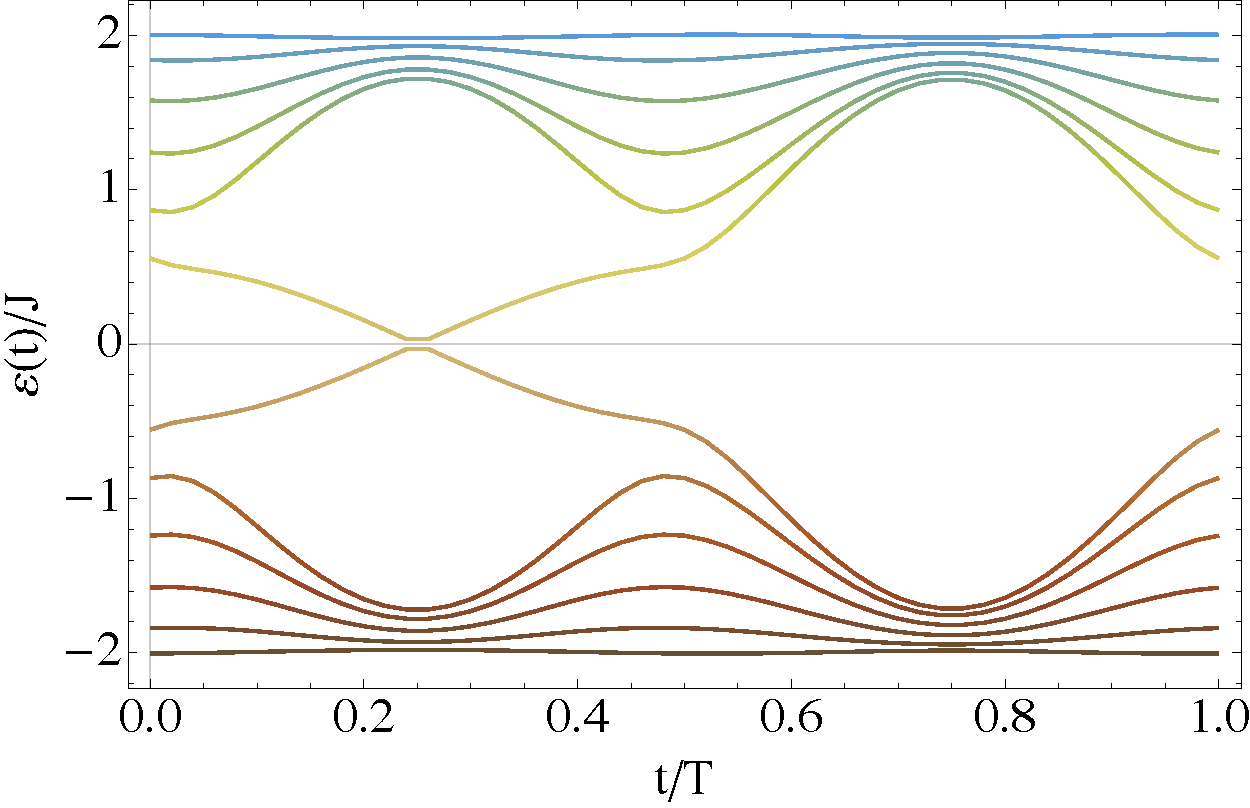
\includegraphics[width=1.\columnwidth]{chap2_topo/rmte_obc_12}
\end{subfigure}
\begin{subfigure}{.48\textwidth}
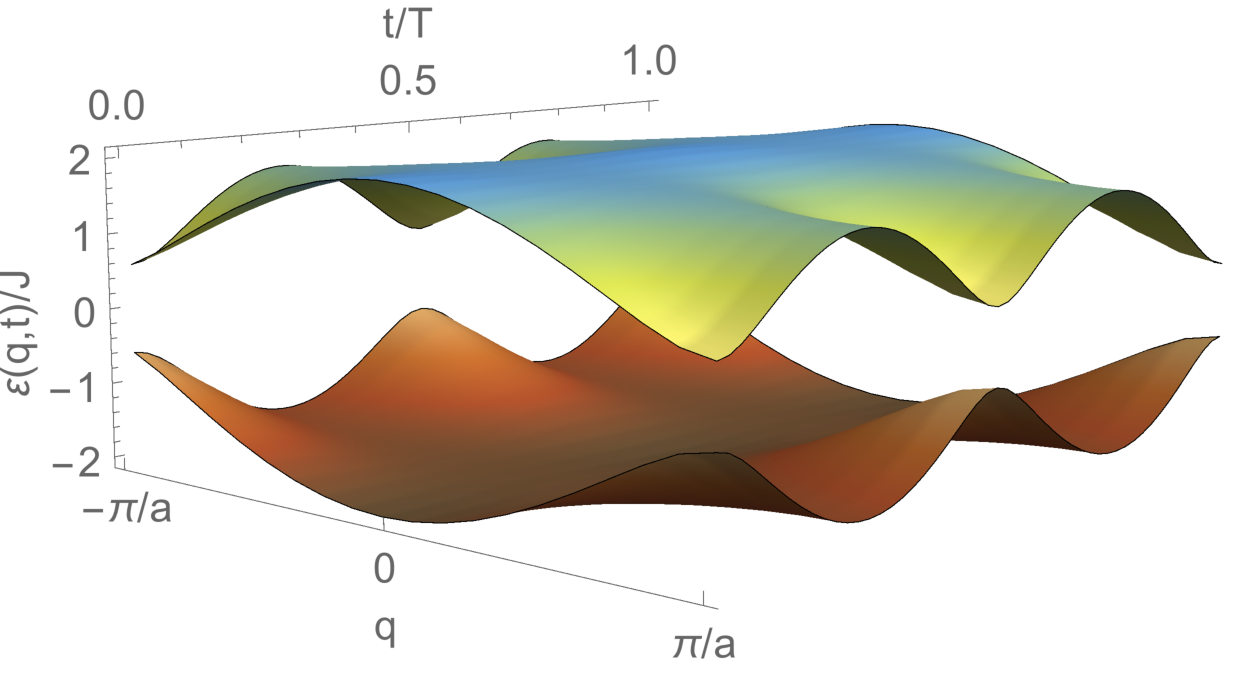
\includegraphics[width=1.\columnwidth]{chap2_topo/rmte_pbc_1}
\end{subfigure}
\caption{Rice-Mele 模型一个典型的非平庸路径演化下开边界条件、周期性边界条件下的能谱。(左)12个格点的开边界条件;(右)周期性边界条件。模型参数:$\delta/J=-0.85$, $\Delta/J=0.5$。}
\label{fig:rmterg}
\end{figure}
对该模型我们画出其沿非平庸路径演化下,分别在开边界条件、周期性边界条件下的能谱,见图 \ref{fig:rmterg} 所示。
从图 \ref{fig:rmterg} (左)可看到,能带中有边界态的存在\footnote{根据 Bulk Edge Correspondence,这也是应该的。}。它们沿着开放的边界\footnote{在此处,时间维度取为周期性,开放的维度即是一维晶格的维度}手征地运动,这就是电荷输运(Charge Pumping)的过程。
\footnote{这样就是经典的 Laughlin's Gauge Argument 所说的事情,可参考\inlinecite{laughlin1981}。这篇文献是作者早期接触到的最经典的几篇文献之一,短小精悍,论述和计算都很简单,但极度不平庸。Laughlin 用非常简单的计算展示了 Quantum Hall 体系中最不平庸的事实,其物理根源与 TKNN 等是一样的。虽然 Laughlin 所讨论的是 Quantum Hall 体系,但实际上和作者这儿演示的是一回事。所有的 Topological Charge Pumping 本质上都是一样的,都是 twisted boundary conditions。}


\begin{figure}[!htb]
\centering
\begin{subfigure}{.45\textwidth}
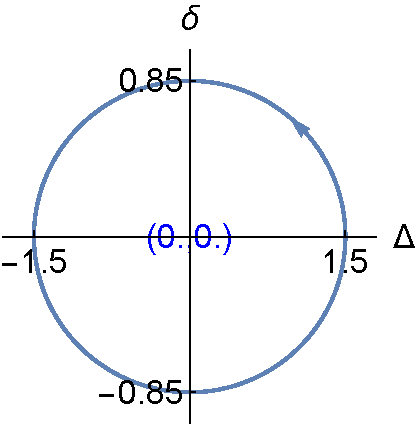
\includegraphics[width=1.\columnwidth]{chap2_topo/tRM_6_evol}
\end{subfigure}
\begin{subfigure}{.45\textwidth}
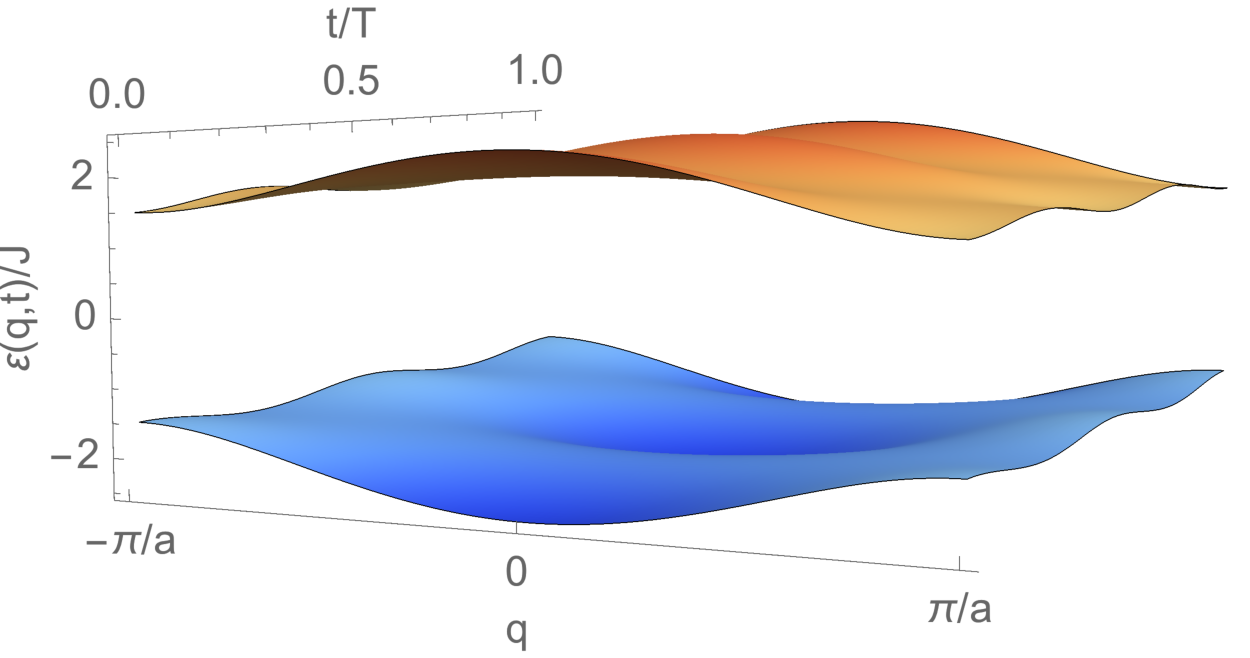
\includegraphics[width=1.\columnwidth]{chap2_topo/tRM_6_eqt}
\end{subfigure}\\
\begin{subfigure}{.45\textwidth}
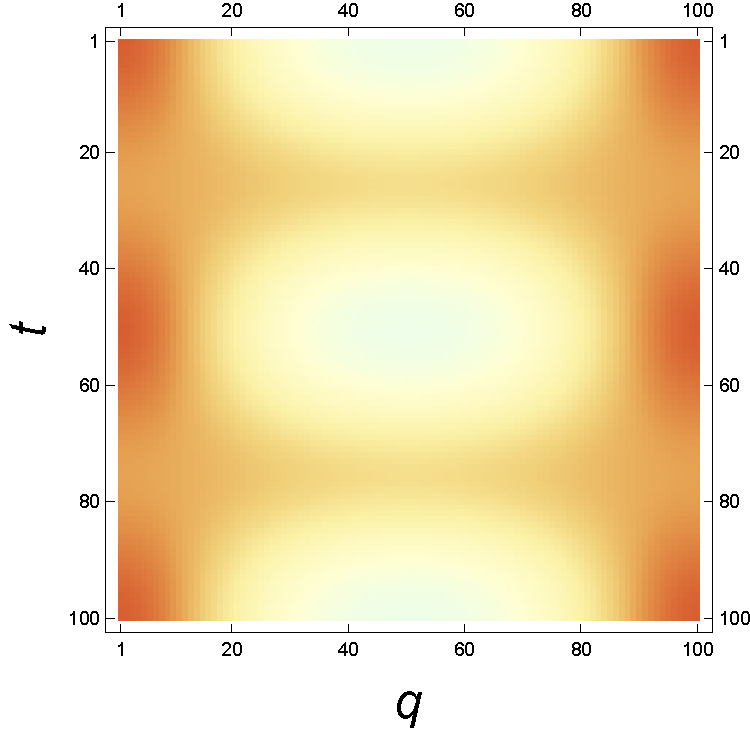
\includegraphics[width=1.\columnwidth]{chap2_topo/tRM_6_bf1}
\end{subfigure}
\begin{subfigure}{.45\textwidth}
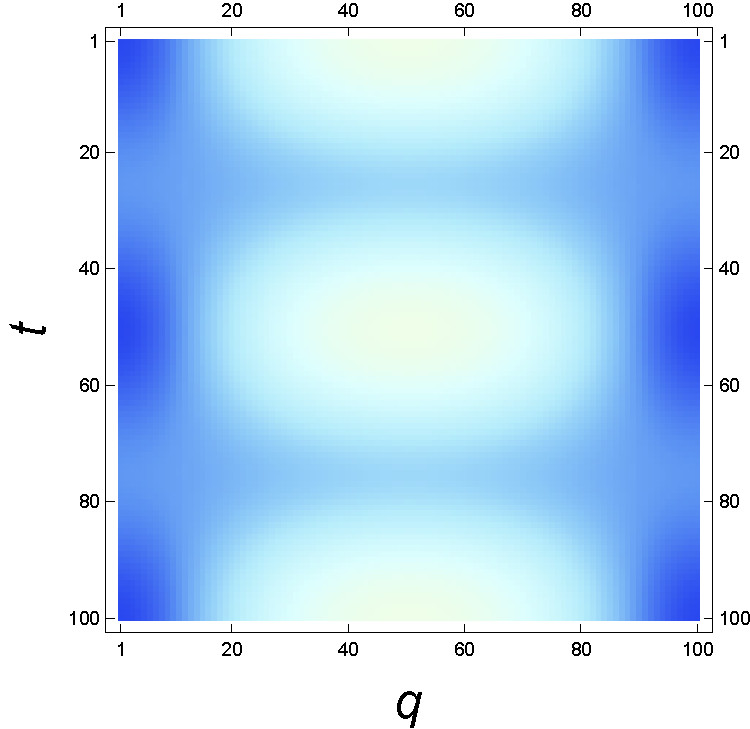
\includegraphics[width=1.\columnwidth]{chap2_topo/tRM_6_bf2}
\end{subfigure}
\caption{Rice-Mele 一个典型的非平庸路径。上栏:左为路径示意图,右为能带结构。下栏:上下两个能带的 Berry 曲率场。模型参数:$\delta/J=-0.85$, $\Delta/J=1.5$。}
\label{fig:rmtberry}
\end{figure}

我们还对一个典型的非平庸演化路径计算了上下两个能带的离散化到 $100\times100$ 的 Berry 曲率场,其积分之后就是两个能带的 Chern 数,分别得 $\pm1$。参见图 \ref{fig:rmtberry}。



\section{ Creutz 梯上的拓扑电子泵}\label{sec:creutz}
这一节我们介绍我们在 Creutz 梯上提出的拓扑电子泵。Creutz 梯的模型由 Michael Creutz 于 1999 年在\inlinecite{creutz1999}文章中提出,旨在研究格点规范理论。原始的 Creutz 模型哈密顿量写作
\begin{align}
\hat{H} =&-\sum_{j} [J_X e^{\ii\theta} \hat{a}_{j+1}^\dag \hat{a}_{j}+J_X e^{-\ii\theta} \hat{b}_{j+1}^\dag \hat{b}_{j} + J_Y \hat{a}_j^\dag \hat{b}_j 
\nonumber\\
&+ J_D \hat{a}_j^\dag \hat{b}_{j+1}+J_D \hat{b}_j^\dag \hat{a}_{j+1} +\textrm{H.c.}]
\end{align}
该模型在特定参数下存在局域化的解,由于 Peierls 相角干涉的原因,局域化在某一对(纵向)格点上的粒子无法跃迁到其他格点\cite{creutz1999}。这让我们联想到 SSH 上类似的情况:SSH 模型中,特定参数下局域化的边界态波函数,当 $J_{\text{out}}\ll J_{\text{in}}$ 时,边界态波函数向体态里延伸的成分非常少(见 \inlinecite{kitaev2001} 中给出的解析解),当极端情况下 $J_{\text{out}}=0$, $J_{\text{in}}=1$ 时,波函数完全局域化在(一对)格点上,无法传播。这启发我们,在 Creutz 模型中也可能存在非平庸的拓扑电子输运的过程。

我们提出以下推广的 Creutz 模型。模型哈密顿量写作,
\begin{align}
\hat{H} =&-\sum_{j} [J_X e^{\ii\theta} \hat{a}_{j+1}^\dag \hat{a}_{j}+J_X e^{-\ii\theta} \hat{b}_{j+1}^\dag \hat{b}_{j} + J_Y e^{-\ii\phi} \hat{a}_j^\dag \hat{b}_j 
\nonumber\\
&+ J_D \hat{a}_j^\dag \hat{b}_{j+1}+J_D \hat{b}_j^\dag \hat{a}_{j+1} +\textrm{H.c.}]
\end{align}
与原始 Creutz 哈密顿量的区别在于在 $J_Y$ 跃迁上加了 $e^{-\ii\phi}$ 的相角。
如图 \ref{fig:creutz:schematic} 所示,图 \ref{fig:creutz:schematic} (a) 为 Creutz 梯的示意图。
\begin{figure}[!htb]
\centering
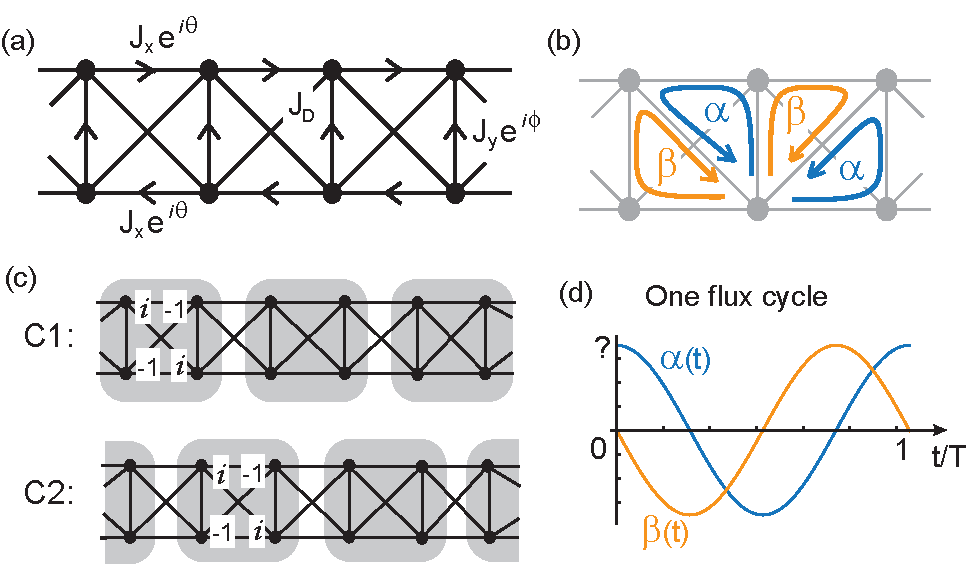
\includegraphics[width=1.\columnwidth]{creutz/fig1}
\caption{Creutz 模型示意图。(a) Creutz 梯晶格模型示意图,该模型由两个 Peierls 相角,单腿上跃迁 $J_Xe^{\ii\theta}$ 中的 $\theta$ 和相邻腿之间跃迁 $J_Ye^{-\ii\phi}$ 中的 $\phi$;(b) 该模型的两个相角也等价于用图示的 $\alpha$, $\beta$ 来刻画;(c) 对于该模型,在特定参数下有局域在方块(plaquette)上的局域态,由于干涉的原因,其不能跃迁到其他格点或方块上\cite{creutz,creutz1999};这种由干涉原因所导致的局域化波函数有两种构型,即图中的 $C_1$ 和 $C_2$,类比于 SSH 模型中调节 $J_1$, $J_2$ 时的两种局域化构型;(d) $\alpha$, $\beta$ 的一种典型的含时依赖周期。(取自\inlinecite{creutz})}
\label{fig:creutz:schematic}
\end{figure}
变换到 $k$-空间,哈密顿量写作
\begin{align}
H(k)=-\begin{pmatrix} 2 J_X \cos(ka-\theta)& 2 J_D\cos(ka)+J_Y e^{-\ii\phi}\\
2 J_D\cos(ka)+J_Y e^{\ii\phi}& 2 J_X \cos(ka+\theta)\end{pmatrix}
\end{align}
以上哈密顿量一般的形式具有 $\sigma_x$, $\sigma_y$, $\sigma_z$ 三个分量,可以预期存在合适的时间依赖路径,使得扩展的 $(k,t)$-二维参数空间具有非零 Chern 数,意即该 $(k,t)$ 向球面的映射能\textit{同向}覆盖一次或几次球面。而根据上一节的结论,非零 Chern 数意味着周期绝热拓扑电子输运的过程。

事实上,我们可以对上述模型的拓扑结构进行全面的分析。对于一维模型,一个可以用来刻画其拓扑结构的量是 Zak 相角\cite{zak1989},实际上是一种能带中的 Berry 相角。Zak 相角本身并不特殊,但选定规范后,Zak 相角的差是一个绝对的数,可以用来区分平庸和非平庸的物态和过程。这方面的实验见\inlinecite{zak-expr-2013}。对于该 Creutz 梯模型,我们给出其参数空间的完整相图,见图 \ref{fig:creutz:topophase} 所示。参数空间中的实线和虚线代表相边界的地方,也就是体系发生简并的地方。因此这些线也叫简并线(degeneracy lines)。在参数空间中穿过实线或虚线时,体系的能隙会关闭再打开,并且发生能带反转(band inversion)\cite{topobook}。围绕这样的简并线形成的参数环路,其含时依赖可以给出拓扑电子输运的行为。
\begin{figure}[!htb]
\centering
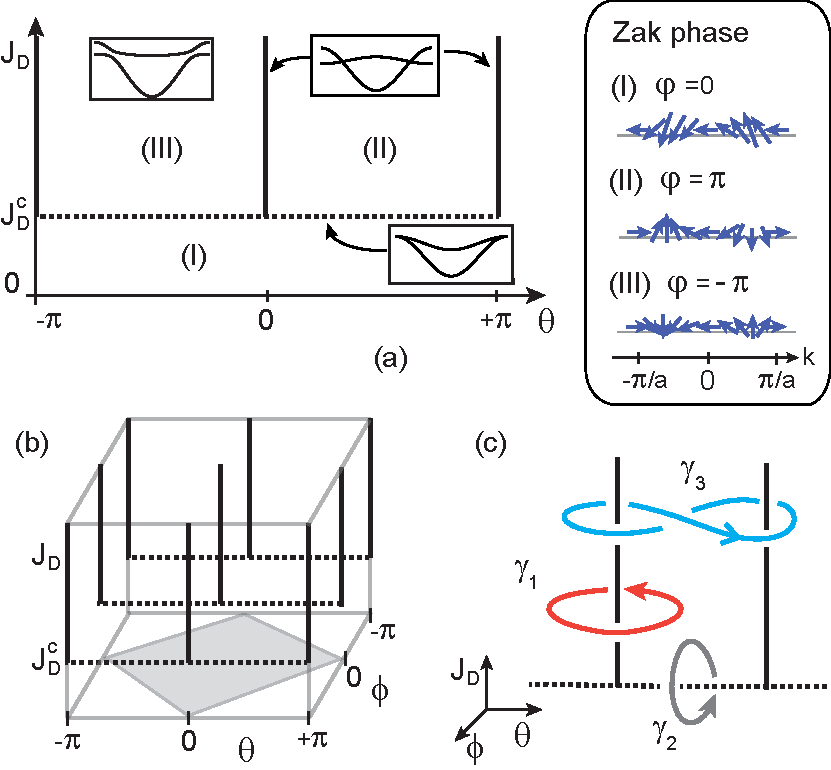
\includegraphics[width=1.\columnwidth]{creutz/fig2}
\caption{Creutz 模型完整拓扑相图。(a) 在 $\phi=0,\pm\pi$ 的平面内,$(J_D, \theta)$ 参数空间的拓扑相图,为 (b) 中之一截面;实线和虚线为相边界,都是体系发生简并的地方(因此也叫 degeneracy lines),在参数空间中穿过实线或虚线,体系发生能隙关闭再打开,并发生能带反转(band inversion);区别在于:实线上的点,能带有两个地方简并,将有两个能隙关闭再打开的情况,并且发生两次(同向的)band inversion,这也是模型中围绕其的非平庸周期演化路径能够发生内禀的以偶数单位拓扑电子输运的根源(见图\ref{fig:creutz:chargepumps});而虚线上的点,能带只有一个地方简并,发生一次能隙关闭再打开,一次能带反转,围绕其的非平庸路径就是上一节提到的 Rice-Mele 型拓扑电子输运;(a) 中的三幅插图标记了不同区域能带和能隙关闭的情况;(b) 模型在 $(J_D, \theta, \phi)$ 空间的完整的拓扑相图;(c) 围绕上述提到的两种 degeneracy lines 几种典型的周期含时演化环路:$\gamma_1$ 具有内禀为偶数单位的新奇拓扑输运,$\gamma_2$ 为普通单位为1的拓扑电子输运(Rice-Mele 型),$\gamma_3$ 为基于 $\gamma_1$ 人为构造的路径,具有单位为4的拓扑电子输运。又上插图展示了几种情况下的 $Zak$ 相角\cite{creutz}。(取自\inlinecite{creutz})}
\label{fig:creutz:topophase}
\end{figure}

图中的实线和虚线代表不同的情况。在实线上,体系有两处地方发生简并
\footnote{见图 \ref{fig:creutz:topophase} (a) 右上插图。},
穿过其上的点将有两个能隙关闭再打开的行为,并且发生两个\textit{同向的}能带反转;而这也正是模型中围绕其的非平庸参数曲线的周期含时路径能够衍生出以偶数为单位的拓扑电子输运的原因,这种偶数单位的拓扑电子输运是内禀的行为,因为事实上绕其\textit{一}圈的参数曲线的电子输运 就为2,Chern 数为2,而绕其一圈已经是约化到最简的路径了,参见图 \ref{fig:creutz:topophase} (c) 中的 $\gamma_1$ 所示。
而在虚线上,体系仅有一处地方发生简并
\footnote{见图 \ref{fig:creutz:topophase} (a) 右下插图。},
穿过其上的点只有一个能隙关闭再打开的行为,只发生一次能带反转,因此围绕其路径 Chern 数为1,拓扑电子输运就是 以1为单位的Rice-Mele 型输运。

图 \ref{fig:creutz:topophase} (b) 给出了三维 $(J_D, \theta, \phi)$ 参数全空间的拓扑相图。图 \ref{fig:creutz:topophase} (a) 展示了其 $\phi=0,\pm\pi$ 时,$(J_D, \theta)$-平面内的情况,几个不同区间和相边界上的能带和能隙关闭情况在插图中给出。相应的,几个区域的 Zak 角在 图 \ref{fig:creutz:topophase} 又上插图中给出示意。图 \ref{fig:creutz:topophase} (c) 画出了几种典型的参数空间闭合环路的示意图,若使体系沿着这些环路具有含时依赖,将会发生拓扑电子输运的行为。其物理根源在上一节中有讨论。其中,$\gamma_1$ 环路的拓扑电子输运以2为单位的,$\gamma_2$ 的以1为单位,而 $\gamma_3$ 相当于两个 $\gamma_1$ 叠加,以 $4$ 为单位。
\footnote{注意,$\gamma_3$ 所绕的方向相反,但并没有抵消掉却是叠加上效果,原因是两条 degeneracy lines 发生的 band inversion 方向恰好相反。因此其相当于两个 $\gamma_1$ 叠加。}


\begin{figure}[!htb]
\centering
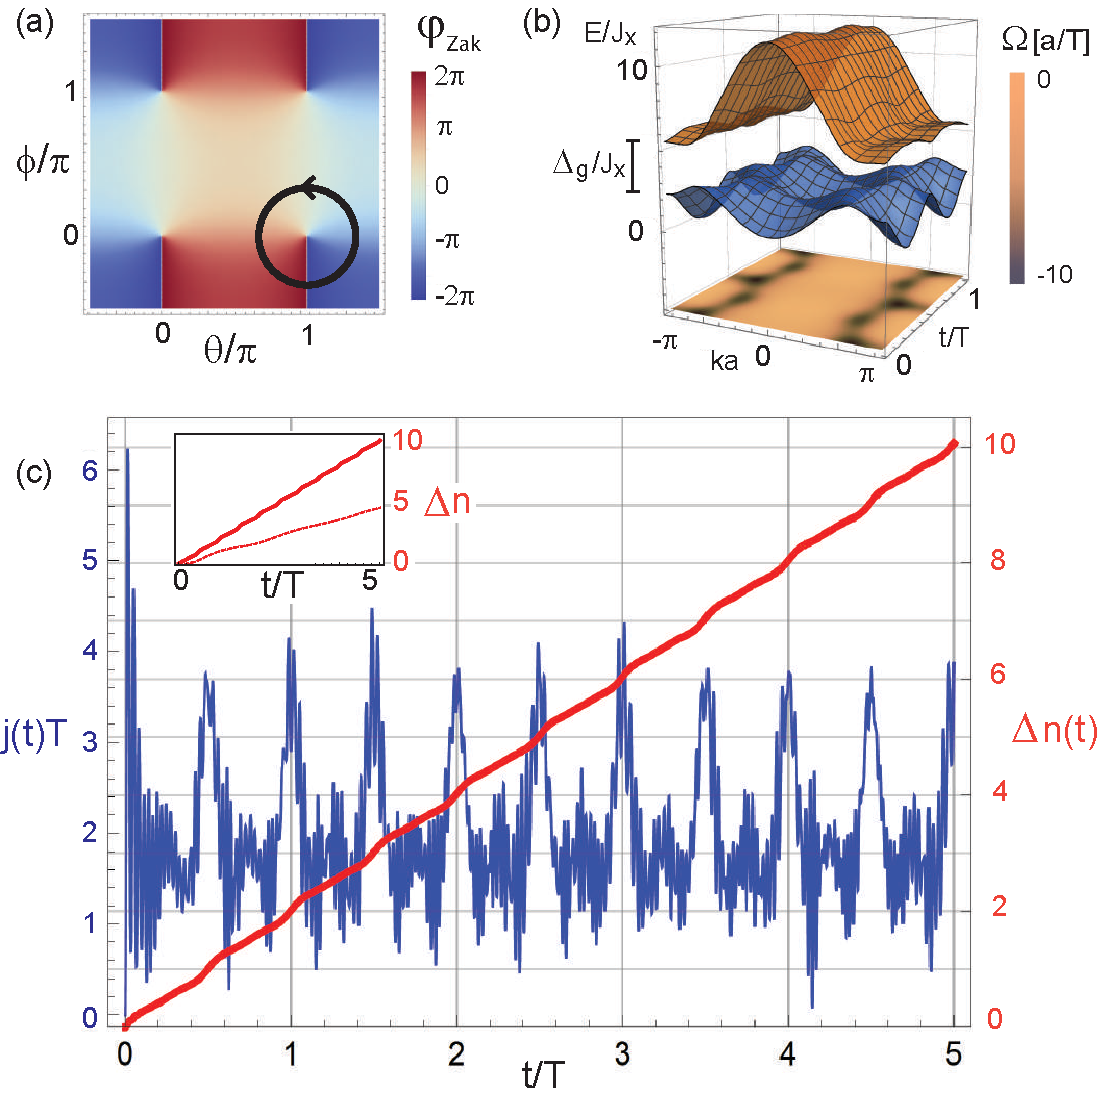
\includegraphics[width=1.\columnwidth]{creutz/fig3}
\caption{Creutz 模型中的拓扑电子输运过程。对于我们发现的内禀偶数为输运单位的新奇拓扑输运现象,我们进行了选取一个典型的路径进行了数值模拟的检验。(a) 含时演化的参数空间,$(\phi, \theta)$-平面,以及其上的Zak相角,黑色带箭头圆圈标记周期含时环路;(b) $(k,t)$ 参数空间的能带结构示意图(上),和基带的 Berry 曲率场(下); (c) 数值模拟含时薛定谔方程的演化的结果,蓝色曲线代表\textit{流}(current)的数值模拟结果(参照左侧蓝色纵坐标),红色曲线为电子输运(或Center-of-Mass)的数值模拟结果(参照右侧红色纵坐标);电子输运为流的积分。可以看出,每个单位周期 $T$,体系输运 $2$ 单位的粒子,而且结果相当得量子化,肉眼可见的精度可以认定为整数。(c)中左上角的插图对比了在相同模型参数下,绝热演化(粗实线)和不绝热演化(细虚线)两种情况的电子输运,对比绝热条件下的高度量子化,非绝热条件下电子的输运不再量子化。这是由于非绝热的驱动下会有将基带电子激发到高带的过程。模型参数:$J_Y/J_X=2$, $J_D/J_X=1.8$, $\hbar\omega/J_x=0.1$(绝热情况),$6.0$(非绝热情况)。(取自\inlinecite{creutz})}
\label{fig:creutz:chargepumps}
\end{figure}

对于这种新奇的内禀输运单位为2的拓扑输运过程,我们选取一组典型的参数进行了数值计算。结果如图 \ref{fig:creutz:chargepumps} 所示。我们选取 $J_Y/J_X=2$, $J_D/J_X=1.8$,并选取图 \ref{fig:creutz:chargepumps} (a) 中所示的黑色带箭头环路作为闭合的周期性含时依赖路径,即
\begin{align}
\phi(t) &= \sin(\omega t) \\ 
\theta(t) &= \cos(\omega t)
\end{align}
其中 $\omega$ 为驱动频率,绝热条件要求 $\hbar\omega\ll J_X, J_Y, J_D$。在该组选定的参数下 $(\phi, \theta)$-平面内的 Zak 相角可以计算出来\cite{creutz},如图 \ref{fig:creutz:chargepumps} (a) 所示。对于现在该组参数下的含时模型,我们解析计算了其能带结构,如图 \ref{fig:creutz:chargepumps} (b) 上部所示。我们也计算了每个能带的 Berry 曲率场和 Chern 数,基带的 Berry 曲率场如图 \ref{fig:creutz:chargepumps} (b) 下部所示。这里用到了 Takahiro Fukui 等人在 2005 年的提出的二维材料的 Chern 数算法\inlinecite{chern2005},详见附录 \ref{sec:chern} 所述
\footnote{在附录 \ref{sec:chern} 中,我们详细讨论了该算法的性质,以及证明了相关的三个定理。这三个定理展示了该算法的有效性,以及量子化、规范不变等性质。我们还开发了分别基于 python3 语言 和 Wolfram Mathematica 语言的专门的程序包,开源地址见\inlinecite{repo-chern}。 }。 Chern 数为 Berry 曲率场的积分,该基带的 Chern 数为2。\footnote{对于这个简单的两能带模型,其 Chern 数本身解析可算。数值方法作为一种检验,与解析方法结果吻合。}

Chern 数为2意味着该路径支持单位为2个电子的周期绝热拓扑电子输运过程。为检验,我们对该组参数下的绝热电子输运过程进行了数值模拟,驱动频率取作
\begin{align}
\hbar\omega/J_X = 0.1
\end{align}
通过数值模拟含时薛定谔方程的演化,我们计算出体系的\textit{流}($j$)和 电子输运($\Delta n$)随时间变化的值,如图 \ref{fig:creutz:chargepumps} (c) 所示。蓝色曲线表示流的值 $j(t)T$,参照左侧蓝色纵坐标;红色曲线表示电子输运的值 $\Delta n(t)$,参照右侧红色总坐标。电子输运为流的积分。
\begin{align}
\Delta n(t) = \int_0^t j(t')dt'
\end{align}

由图 \ref{fig:creutz:chargepumps} (c) 红色曲线可见,在 $\hbar\omega/J_X = 0.1$ 的频率驱动下,每个周期输运的电子为2,而且结果相当量子化,肉眼可见的精度内可以认定为整数。这说明,该频率下体系的演化已经相当绝热。作为对比,我们也计算了“不很绝热”的情况下的电子输运过程,取频率为
\begin{align}
\hbar\omega/J_X = 6.0
\end{align}
数值模拟结果图 \ref{fig:creutz:chargepumps} (c) 左上角插图中的细虚线。与绝热情况下的电子输运对比可见,此时的输运已不再量子化,单位周期输运不再具有整数平台。该频率下前面提到的绝热条件将不被满足,存在从基带到高带的激发过程。






\chapter{光晶格系统中的动力学对称性} \label{chap:dynm}

这一章,我们来讨论光晶格系统中的动力学演化和动力学对称性的问题。作为具体的切入点,我们讨论关于一大类 Hubbard 模型的动力学演化和动力学对称性问题。作为凝聚态物理中许多问题的核心,同时也是超冷原子物理量子模拟的热点,Hubbard 模型本身受到了来自理论层面和实验层面的丰富的研究。 
这一章所讨论的动力学对称性问题为研究 Hubbard 模型的动力学演化提供了新的思路、方法、和视角。

我们将介绍 有 Hubbard 相互作用的体系中一类受保护的动力学对称性(\ref{sec:dynsymm}),和 一类 Fermi-Hubbard 模型中 的 电荷密度波和自旋密度波 的动力学演化,以及相应的电荷输运和自旋输运性质的对称性(\ref{sec:diffusion}),以及证明相关定理。这两个定理给超冷原子物理中的一些实验现象\cite{hubbard-expan-2010,hubbard-expan-2012,mbl1d,twobody-2017,charge-diffusion,spin-diffusion}给出了全新的理解,和可供借鉴的角度。



\section{有 Hubbard 相互作用体系中 受保护的 动力学对称性}\label{sec:dynsymm}

考虑一类有 Hubbard 相互作用的体系。描述这类体系的哈密顿量为如下形式
\begin{align}
\hat{H} = \hat{H}_0 + \hat{H}_I
\end{align}
其中 $H_0$ 为单粒子哈密顿量,$H_I$ 为有格点上的 Hubbard 相互作用的相互作用项。对于自旋1/2的费米子来说,
\begin{align}
\hat{H}_I=U\sum_j\hat{n}_{j\uparrow}\hat{n}_{j\downarrow}
\end{align}
而对于玻色子来说,
\begin{align}
\hat{H}_I=U\sum_{j}\hat{n}_j(\hat{n}_j-1)/2
\end{align}
这其中 $U$ 代表了格点上相互作用的强度。
单粒子哈密顿量部分 $\hat{H}_0$ 可能会存在对称性。我们发现,当 $\hat{H}_0$ 具有某些满足一定条件的对称性时,这类 Hubbard 系统衍生出一种动力学对称性,即在排斥相互作用($+U$)时的动力学演化和在吸引相互作用($-U$)时的动力学演化具有某种对称性。这种衍生的动力学对称性受单粒子哈密顿量 $\hat{H}_0$ 的对称性的保护(支持),我们也称之为受对称性保护的动力学对称性\cite{dynsymm}。下面这个定理表达了这种动力学对称性。
\begin{theorem}\label{thm:dynsymm}
对于如 $\hat{H} = \hat{H}_0 + \hat{H}_I$ 形式的哈密顿量,我们考虑某个初态 $|\psi_i\rangle$ 在其主导下的幺正演化 $|\psi(t)\rangle = e^{\ii\hat{H}t}|\psi_i\rangle$,并且考虑某个可观测量 $\hat{O}$ 在该态下的期望值随时间的演化 $\langle\hat{O}(t)\rangle$。若存在一个幺正算符 $\hat{W}$,使得对$\hat{S}=\hat{R}\hat{W}$,$\hat{R}$ 为(反幺正的)时间反演算符,有
\begin{align}
\{\hat{S}, \hat{H}_0\} &= 0\\
[\hat{S}, \hat{H}_I] &= 0
\end{align}
且 $\hat{O}$ 是 $\hat{S}$-对称的,即
\begin{align}
\hat{S}\hat{O}\hat{S}^{-1} = \pm \hat{O}
\end{align}
和 $|\psi_i\rangle$ 是 $\hat{S}$-不变的,即
\begin{align}
\hat{S}|\psi_i\rangle = e^{\ii\chi}|\psi_i\rangle
\end{align}
那么, $\langle\hat{O}(t)\rangle$ 具有 $U\leftrightarrow-U$ 的对称性:
\begin{align}
\langle\hat{O}(t)\rangle_{+U} = \pm\langle\hat{O}(t)\rangle_{-U}
\end{align}
式中的正负号取决于 $\hat{O}$ 关于 $\hat{S}$ 是奇对称还是偶对称(即$\hat{S}\hat{O}\hat{S}^{-1} = \pm \hat{O}$ 的正负号)。
\end{theorem}

\begin{proof}
直接验证,
\begin{align}
\langle \hat{O}(t)\rangle_{+U}&=\langle\psi_i|e^{\ii \hat{H}t}\hat{O}e^{-\ii \hat{H}t}|\psi_i\rangle\\
&=\langle\psi_i|e^{\ii (\hat{H}_0+\hat{H}_I[U])t}\hat{O}e^{-\ii (\hat{H}_0+\hat{H}_I[U])t}|\psi_i\rangle\\
&=\langle\psi_i|\hat{S}^{-1}\hat{S}e^{\ii (\hat{H}_0+\hat{H}_I[U])t}\hat{S}^{-1}\hat{S}\hat{O}\hat{S}^{-1}\hat{S}e^{-\ii (\hat{H}_0+\hat{H}_I[U])t}\hat{S}^{-1}\hat{S}|\psi_i\rangle\\
&=\langle\psi_i|e^{-\ii\chi}e^{-\ii (-\hat{H}_0+\hat{H}_I[U])t}(\pm \hat{O})e^{\ii (-\hat{H}_0+\hat{H}_I[U])t}e^{\ii\chi}|\psi_i\rangle\\
&=\pm\langle\psi_i|e^{\ii (\hat{H}_0-\hat{H}_I[U])t}\hat{O}e^{-\ii (\hat{H}_0-\hat{H}_I[U])t}|\psi_i\rangle\\
&=\pm\langle\psi_i|e^{\ii (\hat{H}_0+\hat{H}_I[-U])t}\hat{O}e^{-\ii (\hat{H}_0+\hat{H}_I[-U])t}|\psi_i\rangle\\
&=\pm\langle \hat{O}(t)\rangle_{-U}
\end{align}
证毕。
\end{proof}

以上定理对满足对称性条件的混态系综也是成立的。

\begin{corollary}
对于一混合初态,密度矩阵写作 
\begin{align}
\rho_i=\sum_jp_j|\psi_j\rangle\langle\psi_j|
\end{align}
若其中混合的每一个纯态 $|\psi_j\rangle$ 均为 $\hat{S}$-不变的,则该混态满足以上定理 \ref{thm:dynsymm} 的条件,即,对同样满足定理 \ref{thm:dynsymm} 条件的 $\hat{H}$ 和 $\hat{O}$ 上述定理结论成立。
\end{corollary}

\begin{proof}
直接验证,
\begin{align}
\langle \hat{O}(t)\rangle_{\rho_i,+U}&=Tr(\rho_i\hat{O}_{+U}(t))\\
&=\sum_{j}p_j\langle \hat{O}(t)\rangle_{j,+U}\\
&=\sum_jp_j(\pm)\langle \hat{O}(t)\rangle_{j,-U}\\
&=Tr(\pm\rho_i\hat{O}_{-U}(t))\\
&=\pm \langle \hat{O}(t)\rangle_{\rho_i,-U}
\end{align}
证毕。
\end{proof}

对于这个定理,我们给出三类具有代表性的例子进行展示。这三类例子分别对应定理中关于 哈密顿量$\hat{H}$,初态 $|\psi_i\rangle$,和可观测算符 $\hat{O}$ 需满足的三个条件,也分别对应着近年来在冷原子物理中的几个实验\cite{hubbard-expan-2010,hubbard-expan-2012,mbl1d,twobody-2017}。


\subsection{Fermi Hubbard 模型:不同的晶格几何}
首先考虑正方晶格上的 Fermi Hubbard 模型\cite{hubbard-expan-2010,hubbard-expan-2012}。其哈密顿量写作
\footnote{以下在不致混淆的情况下,对算符上的尖帽均隐含不写。}
\begin{align}
    H=-\sum_{\langle i,j\rangle,\sigma}t_{ij}c_{i\sigma}^{\dagger}c_{j\sigma}+h.c.+\sum_iUn_{i\uparrow}n_{i\downarrow}
\end{align}
晶格结构如图 \ref{fig:dynm:fhsquare} 所示。
\begin{figure}[!htb]
\centering
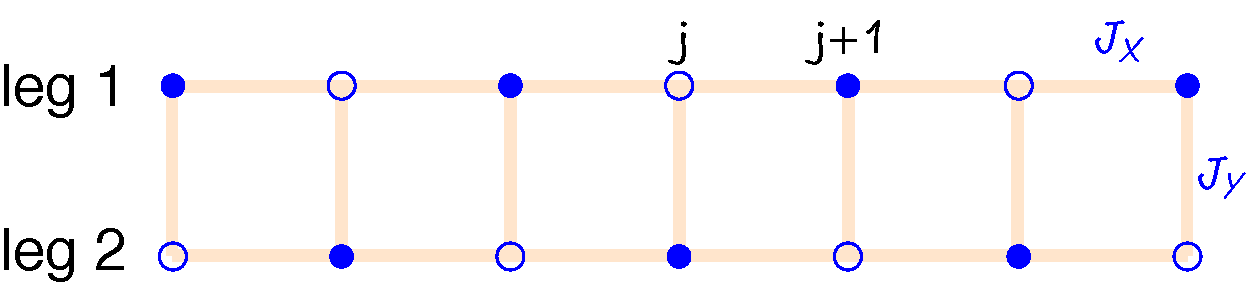
\includegraphics[width=1.0\columnwidth]{chap3_dynm/fhsquare}
\caption{正方晶格上的 Fermi Hubbard 模型示意图。可以看出,正方晶格是二分(bipartite)晶格,意味着晶格可以分为两套$A/B$子格,且每套子晶格中的每个格点只和另一套晶格中的格点相连。}
\label{fig:dynm:fhsquare}
\end{figure}
对该哈密顿量,有如下的幺正变换 $\hat{W}$ 和 时间反演变换 $\hat{R}$,
\begin{align}
& W: \, c_{l\sigma}\rightarrow (-1)^lc_{l\sigma} \\
& K: \,\ii\rightarrow-\ii \\
& R = \ii\sigma_yK 
\end{align}
使得\footnote{这与正方晶格是二分(bipartite)晶格有密切关系。更具体来说,对二分晶格可以定义手征算符 $\Gamma=P_A-P_B$,满足 $\{\Gamma, H_0\}=0$。这使得二分晶格的单粒子谱是正负对称的。一个著名的这样的例子是 SSH 模型。}
\begin{align}
WH_0W^{-1} &= -H_0 \\ 
WH_IW^{-1} &= H_I
\end{align}
继而对 $S=RW$ 有
\begin{align}
SH_0S^{-1} &= -H_0 \\ 
SH_IS^{-1} &= H_I
\end{align}
现在我们来考虑下面这样的初态,
\begin{align}
    |\psi_i\rangle=\sum_j (-1)^jc_{j\uparrow}^{\dagger}c_{j\downarrow}^{\dagger}|0\rangle
\end{align}
容易验证初态在 $S$ 作用下是不变的。同时,我们考虑局域密度的演化,$\langle n_l(t)\rangle$,作为我们的可观测量,那么依据定理 \ref{thm:dynsymm},其含时演化对于排斥相互作用和吸引相互作用具有对称性。且,因 $n_l$ 在 $S$ 下是偶对称的,
\begin{align}
Sn_lS = n_l
\end{align}
应有
\begin{align}
\langle n_l(t)\rangle_{+U} = \langle n_l(t)\rangle_{-U}
\end{align}
我们对 $2\times15$ 个格点的周期性边界条件的体系进行了数值验证。经过严格对角化(Exact Diagonalization,ED)计算,得到几个局域密度观测量在一段时间内的演化,如图 \ref{fig:dynm:fhsed} 所示。
\begin{figure}[!htb]
\begin{subfigure}{.5\textwidth}
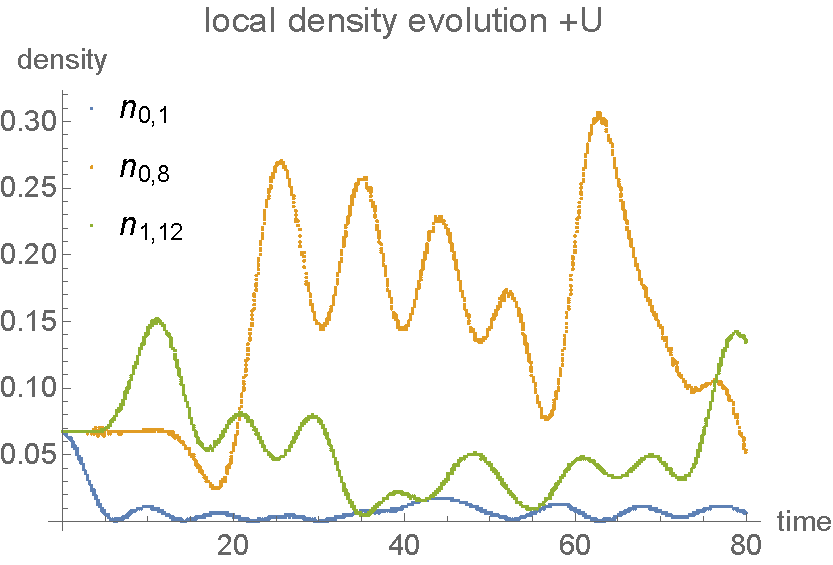
\includegraphics[width=1.\columnwidth]{chap3_dynm/fig_fh1.pdf}
\end{subfigure}
\begin{subfigure}{.5\textwidth}
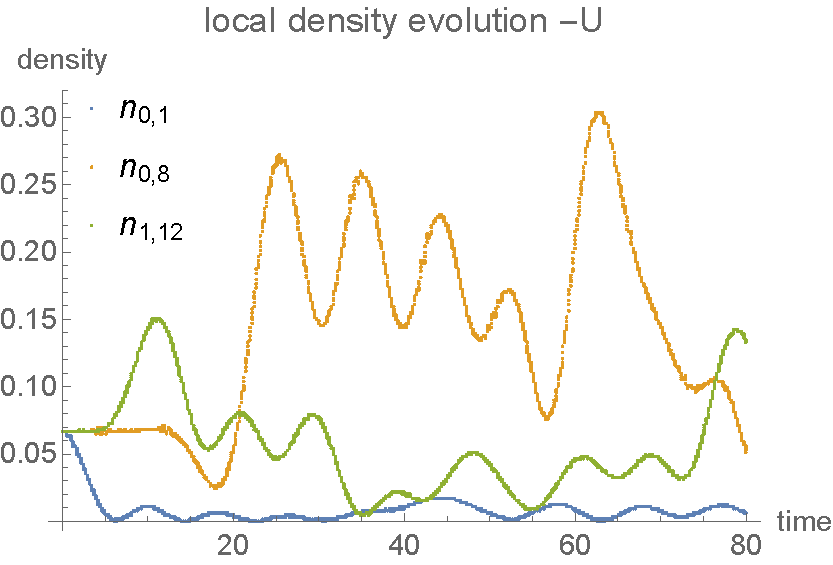
\includegraphics[width=1.\columnwidth]{chap3_dynm/fig_fh2.pdf}
\end{subfigure}\\
\begin{subfigure}{.5\textwidth}
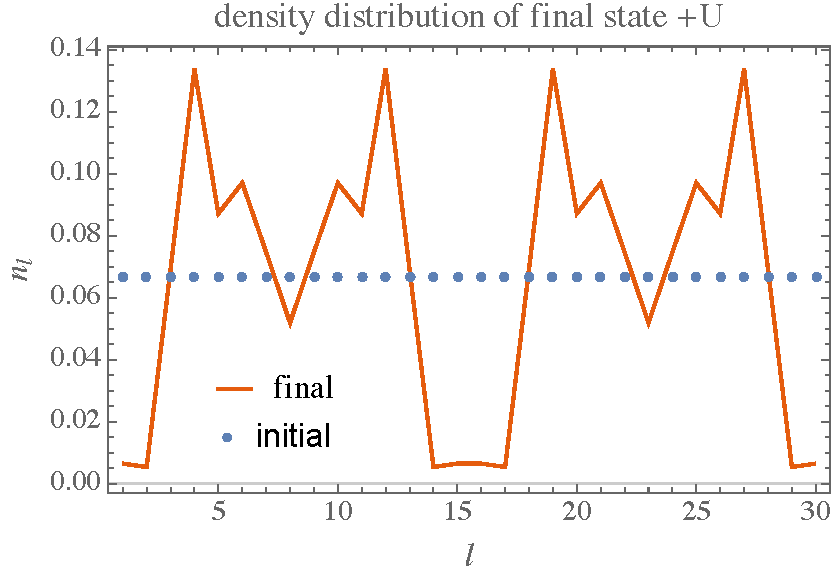
\includegraphics[width=1.\columnwidth]{chap3_dynm/fig_fh3.pdf}
\end{subfigure}
\begin{subfigure}{.5\textwidth}
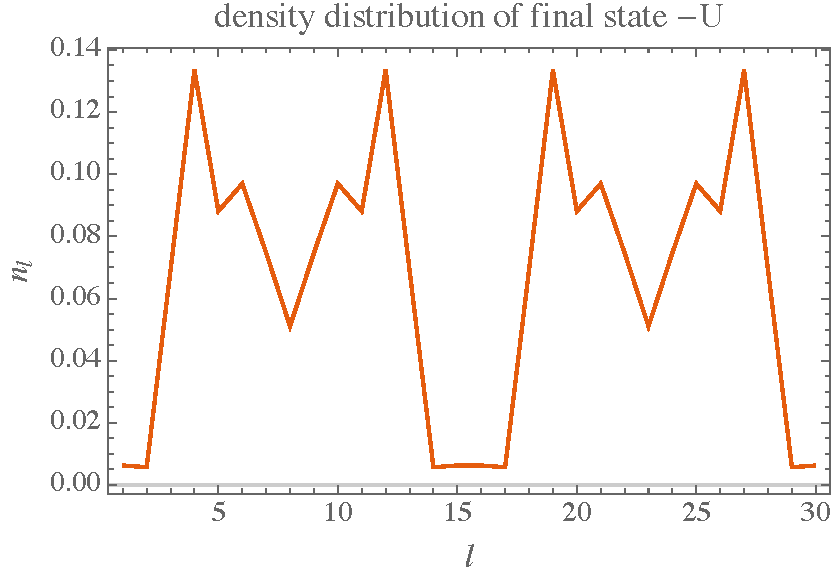
\includegraphics[width=1.\columnwidth]{chap3_dynm/fig_fh4.pdf}
\end{subfigure}
\caption{正方晶格 Fermi Hubbard 模型局域密度观测量的演化。左栏为 $+U$下的演化,右栏为 $-U$下的演化。晶格大小为 $2\times15$ 个格点,周期性边界条件,模型参数为 $J_Y/J_X=1$, $|U|/J_X=10$,初态为 $|\psi_i\rangle=\sum_j (-1)^jc_{j\uparrow}^{\dagger}c_{j\downarrow}^{\dagger}|0\rangle$。横轴时间单位上 $\hbar$ 取作1.}
\label{fig:dynm:fhsed}
\end{figure}

由图 \ref{fig:dynm:fhsed} 所见,数值验证的结果显示,在正方晶格 Fermi Hubbard 模型中,局域密度观测量在该态演化下的期望值确实具有 $+U/-U$ 的对称性,且为偶对称。



下面来考虑三角晶格上的 Fermi Hubbard 模型。哈密顿量写作
\begin{align}
    H=-\sum_{i,j,\sigma}J_Xc_{i,j+1,\sigma}^{\dagger}c_{i,j,\sigma}+J_Yc_{1,j,\sigma}^{\dagger}c_{0,j,\sigma}+J_Yc_{1,j+1,\sigma}^{\dagger}c_{0,j,\sigma}+H.c.+\sum_iUn_{i\uparrow}n_{i\downarrow}
\end{align} 
晶格结构如图 \ref{fig:dynm:fhtriangle} 所示。
\begin{figure}[!htb]
\centering
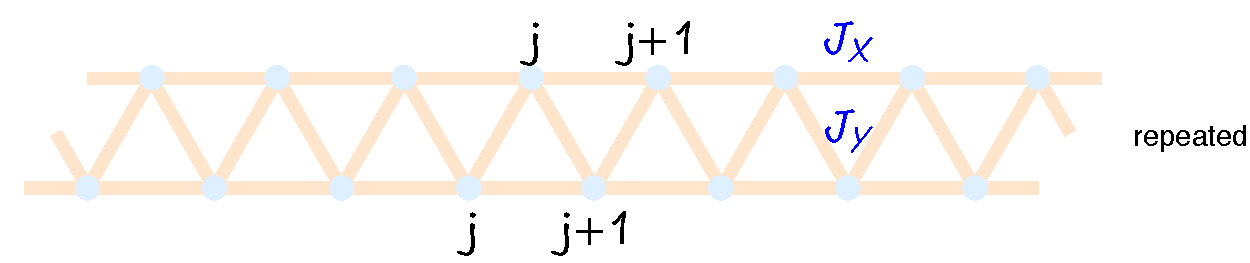
\includegraphics[width=1.0\columnwidth]{chap3_dynm/fhtriangle}
\caption{三角晶格上的 Fermi Hubbard 模型示意图。三角晶格不是二分晶格,无法分成$A/B$ 两套子格使其满足每套子晶格中的每个格点只和另一套晶格中的格点相连。}
\label{fig:dynm:fhtriangle}
\end{figure}

对于三角晶格,上述 $W$ 和 $S$ 将不再满足定理条件,哈密顿量在 $S$ 下不具有上面描述的对称性。因此可以预见,定理结论不再成立,即,选择同样初态和同样的可观测算符,如局域密度算符,其随时间演化的期望值不具有 $+U/-U$ 对称性。

作为验证,我们同样进行了严格对角化(ED)计算,同样对于一个 $2\times15$ 大小周期性边界条件的晶格。如图 \ref{fig:dynm:fhted} 所示,局域密度可观测量在该态下的期望值确实不再具有 $+U/-U$ 对称性。

\begin{figure}[!htb]
\begin{subfigure}{.5\textwidth}
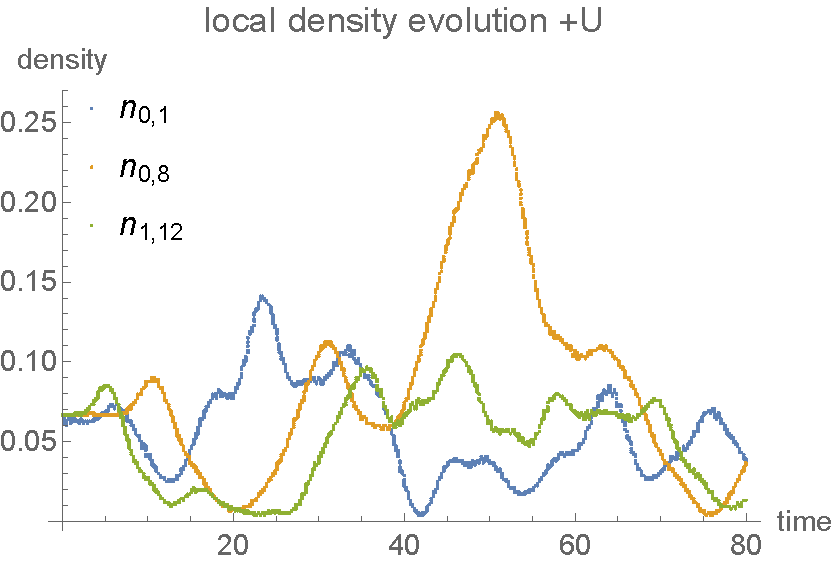
\includegraphics[width=1.\columnwidth]{chap3_dynm/fig_fhtri1.pdf}
\end{subfigure}
\begin{subfigure}{.5\textwidth}
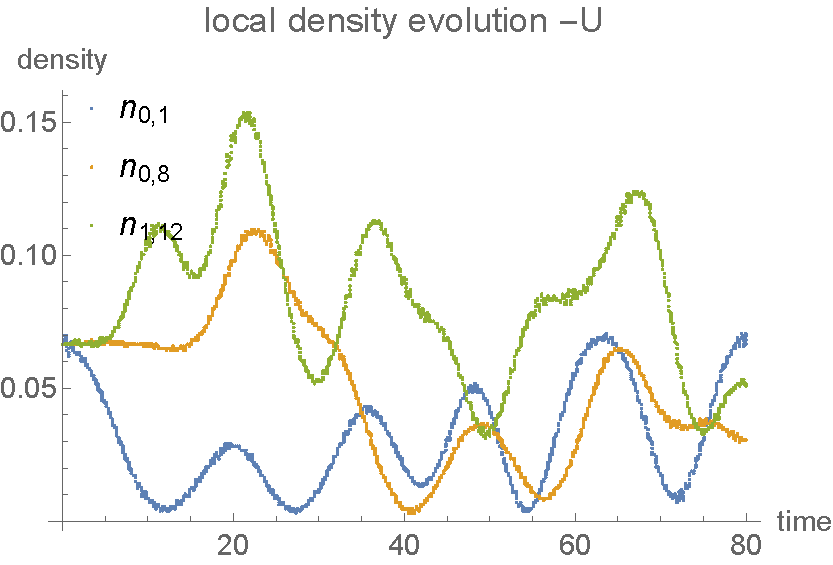
\includegraphics[width=1.\columnwidth]{chap3_dynm/fig_fhtri2.pdf}
\end{subfigure}\\
\begin{subfigure}{.5\textwidth}
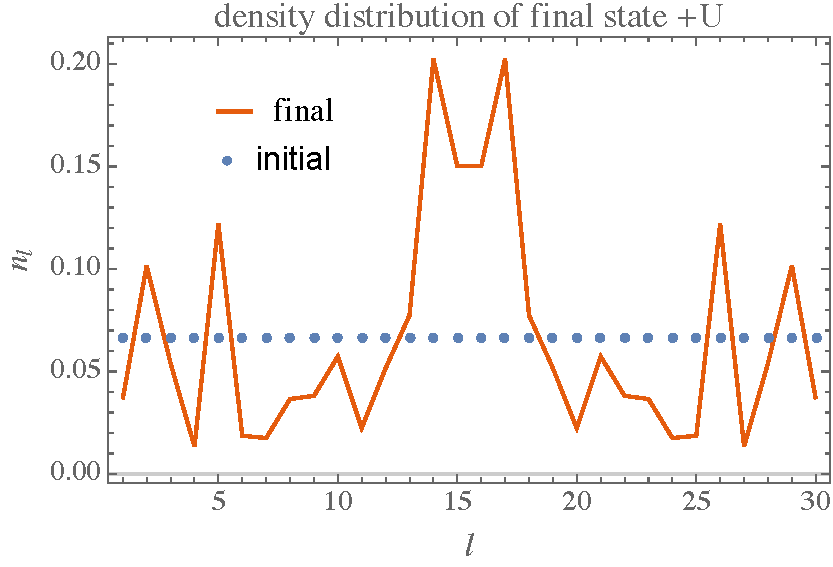
\includegraphics[width=1.\columnwidth]{chap3_dynm/fig_fhtri3.pdf}
\end{subfigure}
\begin{subfigure}{.5\textwidth}
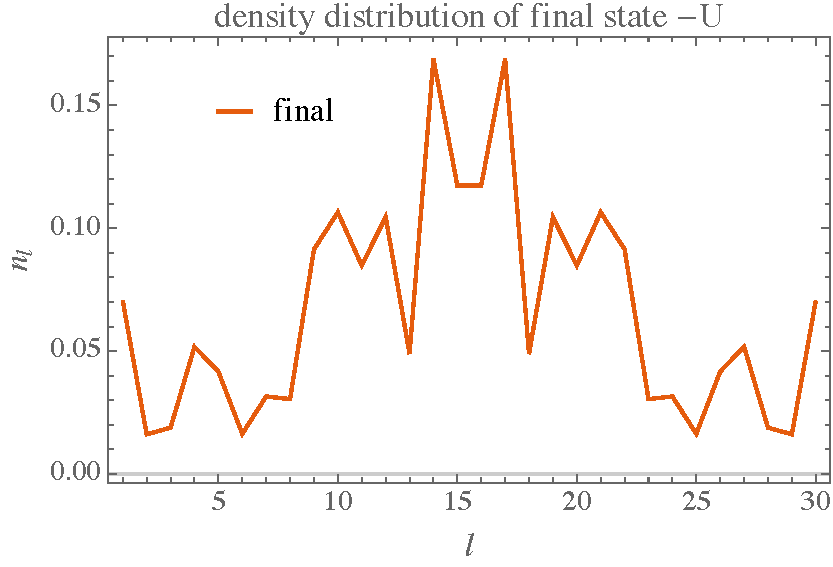
\includegraphics[width=1.\columnwidth]{chap3_dynm/fig_fhtri4.pdf}
\end{subfigure}
\caption{三角晶格 Fermi Hubbard 模型局域密度观测量的演化。左栏为 $+U$下的演化,右栏为 $-U$下的演化。晶格大小为 $2\times15$ 个格点,周期性边界条件,模型参数为 $J_Y/J_X=1$, $|U|/J_X=10$,初态为 $|\psi_i\rangle=\sum_j (-1)^jc_{j\uparrow}^{\dagger}c_{j\downarrow}^{\dagger}|0\rangle$。横轴时间单位上 $\hbar$ 取作1.}
\label{fig:dynm:fhted}
\end{figure}



\subsection{玻色子带磁通的 Hubbard 晶格:不同的初态}
下面来考虑在正方晶格上玻色子的带磁通的的 Hubbard 模型\cite{twobody-2017}。哈密顿量写作
\begin{align}
H=&-\sum_jJ_X(e^{-\ii\phi/2}a^{\dagger}_{j+1}a_j+e^{\ii\phi/2}b^{\dagger}_{j+1}b_j)+J_Ya_j^{\dagger}b_j+h.c. 
% \\&\qquad\qquad\qquad\qquad
+\dfrac{U}{2}\sum_jn_j^{(a)}(n_j^{(a)}-1)+n_j^{(b)}(n_j^{(b)}-1)
\end{align}
晶格结构如图 \ref{fig:dynm:fluxladder} (a) 所示。
\begin{figure}[!htb]
\centering
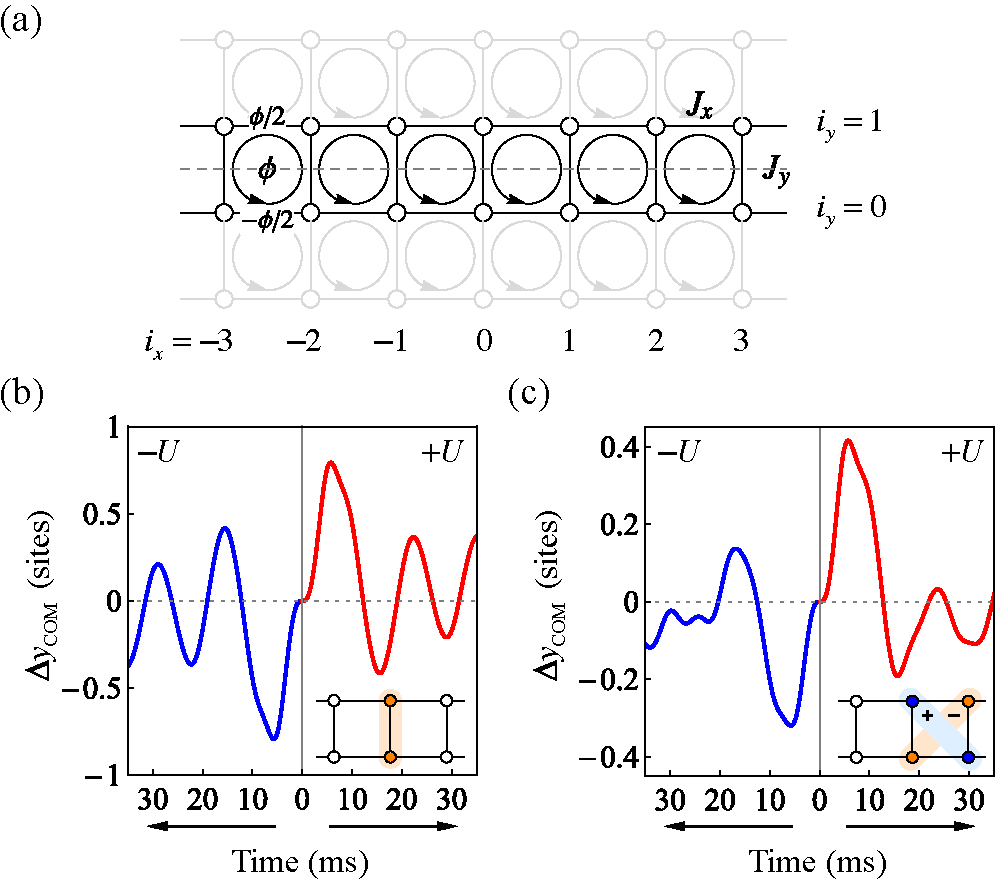
\includegraphics[width=1.0\columnwidth]{dynsymm/example2}
\caption{正方晶格上玻色子的带磁通的的 Hubbard 模型。(a) 晶格结构示意图;(b)初态 \ref{eq:state1} 演化下 $\Delta y_{\text{c.m.}}(t)$ 期望值;(c)初态 \ref{eq:state2} 演化下 $\Delta y_{\text{c.m.}}(t)$ 的期望值。 模型参数见 \inlinecite{dynsymm}(取自\inlinecite{dynsymm})}
\label{fig:dynm:fluxladder}
\end{figure}
考虑如下的幺正变换
\begin{align}
&\hat{W}^{-1}\hat{c}_{i_x,i_y,\sigma}\hat{W}=(-1)^{i_x+i_y}\hat{c}_{i_x,1-i_y,\sigma},  \label{W2} 
\end{align}
容易验证,该幺正变换满足定理 \ref{thm:dynsymm} 所述条件\cite{dynsymm}。
先考虑如下两种初态。第一种
\begin{align}\label{eq:state1}
|\Psi_0\rangle&=\frac{1}{2}(\hat{c}^\dag_{0,0}+\hat{c}^\dag_{0,1})(\hat{c}^\dag_{0,0}-\hat{c}^\dag_{0,1})|0\rangle\nonumber\\
&=\hat{c}^\dag_{0,0}\hat{c}^\dag_{0,1}|0\rangle.
\end{align}
容易验证,该算符具有 $S$-不变性。现在考虑以该态作为初态的幺正演化,演化一段时间后其左右两半的质心(Center-of-Mass)位置的期望值,定义如下的观测量
\begin{align}
\Delta y_{\text{c.m.}}(t)=\frac{\langle \hat{O}^R_{-}(t)\rangle}{\langle \hat{O}^R_{+}(t)\rangle}-\frac{\langle \hat{O}^L_{-}(t)\rangle}{\langle \hat{O}^L_{+}(t)\rangle}
\end{align}
其中
\begin{align}
&\hat{O}^R_{\pm}=\sum\limits_{i_x>0}(\hat{n}_{i_x,i_y=1}\pm \hat{n}_{i_x,i_y=0}), \\
&\hat{O}^L_{\pm}=\sum\limits_{i_x<0}(\hat{n}_{i_x,i_y=1}\pm \hat{n}_{i_x,i_y=0}). 
\end{align}
可以直接验证,
\begin{align}
\hat{S}^{-1}\hat{O}^{R/L}_{\pm}\hat{S}=\pm \hat{O}^{R/L}_{\pm},
\end{align}
因此,
\begin{align}
\Delta y_{\text{c.m.}}(t)|_{+U}=-\Delta y_{\text{c.m.}}(t)|_{-U}
\end{align}
对此,我们做了数值检验。经过严格对角化计算,该态下的 $\Delta y_{\text{c.m.}}(t)$ 期望值确实具有 $+U/-U$ 对称性,且为奇对称,如图 \ref{fig:dynm:fluxladder}(b) 所示。

现在考虑另一种初态,
\begin{align}\label{eq:state2}
|\Psi_0\rangle&=\frac{1}{2}(\hat{c}^\dag_{0,1}+\hat{c}^\dag_{1,0})(\hat{c}^\dag_{1,1}-\hat{c}^\dag_{0,0})|0\rangle,
\end{align}
可以直接验证,该态并不具备定理 \ref{thm:dynsymm} 所述 $S$-不变性,因此定理结论不成立,$\Delta y_{\text{c.m.}}(t)$ 在其演化下的期望值不具有 $+U/-U$ 对称性。数值模拟结果见图 \ref{fig:dynm:fluxladder} (c)。




\subsection{Aubry-Andre 模型:不同的可观测量的对称性}
下面来考虑 Aubry-Andre 模型。模型的哈密顿量写作
\begin{align}
\hat{H}_0=\sum\limits_{i,\sigma}-J(\hat{c}^\dag_{i,\sigma}\hat{c}_{i+1,\sigma}+\text{h.c.})+\Delta\cos(2\pi\beta i+\theta)\hat{n}_{i,\sigma} + U\sum_j\hat{n}_{j\uparrow}\hat{n}_{j\downarrow}
\end{align}
晶格结构如图 \ref{fig:dynm:aa} (a) 所示。这是一个利用不公度的晶格实现准无序体系的模型\cite{mbl1d}。
\begin{figure}[!htb]
\centering
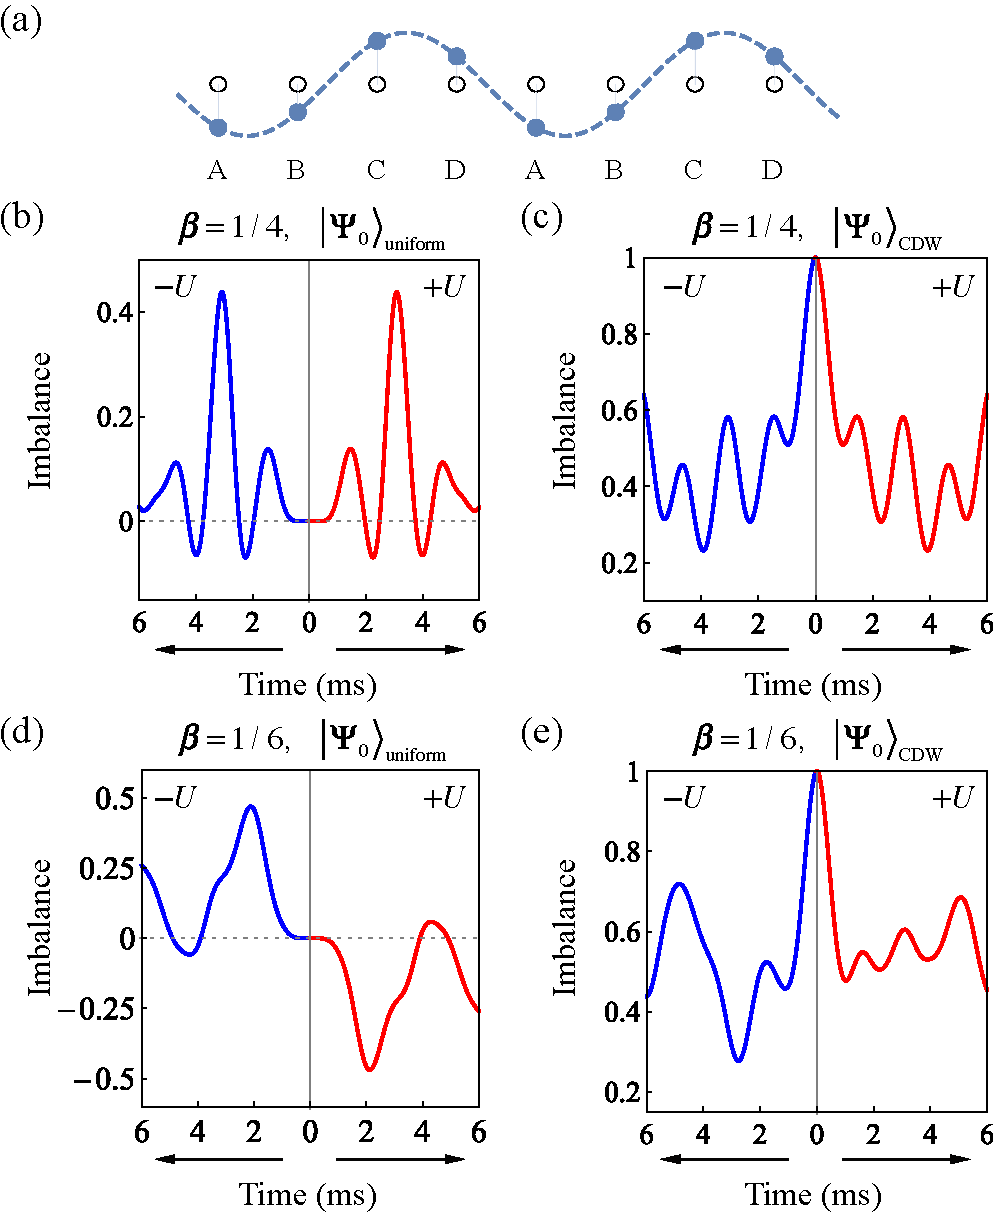
\includegraphics[width=1.0\columnwidth]{dynsymm/example3}
\caption{Aubry-Andre Hubbard 模型。(a) 晶格结构示意图;(b)(c) $\beta=1/4$ 时,两种初态演化下非平衡观测量的期望值;(d)(e) $\beta=1/6$ 时,两种初态演化下非平衡可观测量的期望值。利用严格对角化进行数值模拟。模型参数见 \inlinecite{dynsymm}(取自\inlinecite{dynsymm})}
\label{fig:dynm:aa}
\end{figure}

现在考虑一种非平衡观测量\cite{mbl1d},定义如下
\begin{equation}
\hat{\mathcal{I}}=\frac{\sum_{i\subset \text{even}}\hat{n}_{i\sigma}-\sum_{i\subset \text{odd}}\hat{n}_{i\sigma}}{\sum_{i\subset \text{even}}\hat{n}_{i\sigma}+\sum_{i\subset \text{odd}}\hat{n}_{i\sigma}}.
\end{equation}
和两种初态,
\begin{align}
&|\Psi_0\rangle_{\text{uniform}}=\frac{1}{\sqrt{N}}\sum\limits_{i=1}^{N}\hat{c}^\dag_{i\uparrow}\hat{c}^\dag_{i\downarrow}|0\rangle;\\
&|\Psi_0\rangle_{\text{CDW}}=\frac{1}{\sqrt{N/2}}\sum\limits_{i=1,i\subset \text{odd}}^{N}\hat{c}^\dag_{i\uparrow}\hat{c}^\dag_{i\downarrow}|0\rangle.
\end{align}
考虑该可观测量在这两种态的幺正演化下的期望值。为了发现其动力学演化的精确关系,我们现在利用定理 \ref{thm:dynsymm}。现在需要找到合适的 $\hat{S}$ 也就是 $\hat{W}$。

这里的晶格不公度参数 $\beta$ 总可以写为有理数,或用有理数近似逼近。即 
\begin{align}
\beta=p/q
\end{align}
对 $p,q$ 不同的情况,我们寻找不同的 $\hat{W}$。
\begin{enumerate}
\item $p$ 是奇数,$q$ 是偶数,且 $q/2$ 是偶数。
存在
\begin{align}
\hat{W}^{-1}\hat{c}_{i,\sigma}\hat{W}=(-1)^{i}\hat{c}_{i+q/2,\sigma}.  \label{W3} 
\end{align}
模型在其变换下具有不变性。
使得 $\hat{\mathcal{I}}$ 在 $\hat{S}$ 下是偶对称,且 $|\Psi_0\rangle_{\text{uniform}}$ 和 $|\Psi_0\rangle_{\text{CDW}}$ 态均为 $\hat{S}$-不变的。因此,这种情况下,$\hat{\mathcal{I}}$ 在两种初态幺正演化下的期望值均有 $+U/-U$ 对称性,且为偶对称。见图 \ref{fig:dynm:aa}(b)(c)。

\item $p$ 是奇数,$q$ 是偶数,且 $q/2$ 是奇数。
这时,上式的 $\hat{W}$ 还是满足模型的对称性的。但此时,$\hat{\mathcal{I}}$ 在 $\hat{S}$ 下是奇对称,且只有 $|\Psi_0\rangle_{\text{uniform}}$ 在其下不变,$|\Psi_0\rangle_{\text{CDW}}$ 在其变换下不再具有不变性。因此,这种情况下,$\hat{\mathcal{I}}$ 在 $|\Psi_0\rangle_{\text{uniform}}$ 幺正演化下的期望值具有 $+U/-U$ 对称性,且为奇对称,而在 $|\Psi_0\rangle_{\text{CDW}}$ 幺正演化下的期望值不再具有 $+U/-U$ 对称性。见图 \ref{fig:dynm:aa}(d)(e)。

\item $q$ 是奇数。这种情况下无法找到满足定理 \ref{thm:dynsymm} 所述的 $\hat{S}$。非平衡可观测量 $\mathcal{I}$ 的含时演化不具有 $+U/-U$ 对称性。
\end{enumerate}



\section{Fermi-Hubbard 模型中电荷输运与自旋输运的对称性}\label{sec:diffusion}

Fermi Hubbard 模型中的电荷输运与自旋输运问题是许多凝聚态物理所关注的问题的核心。特别是,最近在冷原子物理中也有若干实验研究在光晶格模拟中的电荷输运问题\cite{charge-diffusion}和自旋输运问题\cite{spin-diffusion},并对电荷输运扩散系数和自旋输运扩散系数\cite{spin-diffusion}进行了研究。

受上述实验的启发,我们发现了在一类二分晶格 Fermi Hubbard 模型中电荷和自旋在动力学性质方面的对称性\cite{diffusion}。下面我们将讨论这种对称性,并给出一定的精确关系。

我们考虑二分晶格上的 Fermi Hubbard 模型,其哈密顿量写作
\begin{align}
    \hat{H} = \sum_{\langle i,j\rangle,\sigma} -t\hat{c}_{i\sigma}^{\dagger}\hat{c}_{j\sigma} + \sum_{i} U \hat{n}_{i\uparrow}\hat{n}_{i\downarrow} 
\end{align}
这里 $\langle i,j\rangle$ 标示最近邻格点,其中 $i\in A$ 而 $j\in B$。

如果考虑多体系统,则可以通过调节化学势来改变体系的总粒子数。这是可将哈密顿量写作
\begin{align}
    \hat{H} = \sum_{\langle i,j\rangle,\sigma} -t\hat{c}_{i\sigma}^{\dagger}\hat{c}_{j\sigma} + \sum_{i} U \hat{n}_{i\uparrow}\hat{n}_{i\downarrow} - \sum_i\mu_i\hat{n}_i
\end{align}
这里 $\mu_i$ 是局域的化学势,或者
\begin{align}
    \hat{H} = \sum_{\langle i,j\rangle,\sigma} -t\hat{c}_{i\sigma}^{\dagger}\hat{c}_{j\sigma} + \sum_{i} U \hat{n}_{i\uparrow}\hat{n}_{i\downarrow} -\mu\hat{N}
\end{align}
这里 $\mu$ 是总化学势。对于一个半填充的体系,$\mu=N/2$,或者说,
\begin{align}
    \hat{H} = \sum_{\langle i,j\rangle,\sigma} -t\hat{c}_{i\sigma}^{\dagger}\hat{c}_{j\sigma} + \sum_{i} U \left(\hat{n}_{i\uparrow}-\dfrac{1}{2}\right)\left(\hat{n}_{i\downarrow}-\frac{1}{2}\right) 
\end{align}

现在定义一组粒子空穴变换,
\begin{definition}
粒子空穴变换 $\mathcal{P}$ 为:
\begin{align}
    \mathcal{P} : \  \  
    & \hat{c}_{i\uparrow} \rightarrow (-1)^{i} \hat{c}_{i\uparrow}^{\dagger},  \nonumber\\
    & \hat{c}_{i\downarrow} \rightarrow \hat{c}_{i\downarrow}. 
\end{align}
\end{definition}
或者更具体可以写作,
\begin{align}
    \mathcal{P} |n_{i\uparrow} = 0\rangle = |n_{i\uparrow} = 1\rangle, \  \  
    \mathcal{P} |n_{i\uparrow} = 1\rangle = |n_{i\uparrow} = 0\rangle. 
\end{align}

\begin{lemma}\label{lemma1}
对于半填充的二分 Fermi Hubbard 模型,上述粒子空穴变换将 $+U$ 的模型映射为 $-U$ 的模型,反之亦然。
\begin{align}
\mathcal{P}: H(+U) \leftrightarrow H(-U)
\end{align}
\end{lemma}

\begin{proof}
由 $\mathcal{P}$ 的定义易得,
\begin{align}
\mathcal{P}\left(\sum_{\langle i,j\rangle,\sigma} -t\hat{c}_{i\sigma}^{\dagger}\hat{c}_{j\sigma}\right) \mathcal{P}^{-1} = \sum_{\langle i,j\rangle,\sigma} -t\hat{c}_{i\sigma}^{\dagger}\hat{c}_{j\sigma} 
\end{align}
而对所有格点 $i$ 都有
\begin{align}
\mathcal{P}\left(\hat{n}_{i\uparrow}-\dfrac{1}{2}\right)\left(\hat{n}_{i\downarrow}-\frac{1}{2}\right) \mathcal{P}^{-1} &= \left(\dfrac{1}{2}-\hat{n}_{i\uparrow}\right)\left(\hat{n}_{i\downarrow}-\frac{1}{2}\right) \\
&= - \left(\hat{n}_{i\uparrow}-\dfrac{1}{2}\right)\left(\hat{n}_{i\downarrow}-\frac{1}{2}\right)
\end{align}
因此有
\begin{align}
\mathcal{P} \left(\sum_{i} U \left(\hat{n}_{i\uparrow}-\dfrac{1}{2}\right)\left(\hat{n}_{i\downarrow}-\frac{1}{2}\right) \right) \mathcal{P}^{-1} = - \sum_{i} U \left(\hat{n}_{i\uparrow}-\dfrac{1}{2}\right)\left(\hat{n}_{i\downarrow}-\frac{1}{2}\right) 
\end{align}
即,
\begin{align}
\mathcal{P}H(+U)\mathcal{P}^{-1} = H(-U)
\end{align}
证毕。
\end{proof}

现引入局域电荷密度算符和局域自旋密度算符的定义。
\begin{definition}
局域电荷密度算符 $\hat{n}_{i}$ 定义为 $\hat{n}_{i} = \hat{n}_{i\uparrow} + \hat{n}_{i\downarrow}$。
局域自旋密度算符 $\hat{S}_{i}$ 定义为 $\hat{S}_{i}=\hat{n}_{i\uparrow} - \hat{n}_{i\downarrow}$。
\end{definition}

\begin{lemma}\label{lemma2}
$\mathcal{P}$ 将二者如下映射:
\begin{align}
\mathcal{P}\hat{S}_i\mathcal{P}^{-1} = 1 - \hat{n}_i
\end{align}
\end{lemma}
可直接验证,证明略。

下面来考虑两种类型的 Fock 态,一种具有均匀的局域电荷密度,另一种具有均匀的局域自旋密度。例如,下面两个给出两个半填充的一维晶格上的例子,
\begin{align}
|\uppsi_1\rangle &= \prod_{i\leq\frac{N}{2}}\hat{c}_{i\uparrow}^{\dagger}\hat{c}_{i\downarrow}^{\dagger}|0\rangle \\
|\uppsi_2\rangle &= \prod_{i\leq\frac{N}{2}}\prod_{j\geq\frac{N}{2}}\hat{c}_{i\downarrow}^{\dagger}\hat{c}_{j\uparrow}^{\dagger}|0\rangle
\end{align}
其中 $|\psi_1\rangle$ 具有均匀的局域自旋密度,和不均匀的局域电荷密度,而 $|\psi_2\rangle$ 具有均匀的局域电荷密度,和不均匀的局域自旋密度。

我们下面定义一类自旋密度波Fock态和电荷密度波Fock态。
\begin{definition}\label{def:state12}
对于 Fock 态 $|\psi\rangle = \prod_{i\sigma}\hat{c}_{i\sigma}^{\dagger}|0\rangle$,SDW 类为满足以下两个条件的态:

i) $\forall i, \langle\psi|\hat{S}_i|\psi\rangle = 0$, 

ii) $\exists i, \langle\psi|\hat{n}_i|\psi\rangle \neq 1$. 

CDW 类为满足以下两个条件的态:

i) $\forall i, \langle\psi|\hat{n}_i|\psi\rangle = 1$, 

ii) $\exists i, \langle\psi|\hat{S}_i|\psi\rangle \neq 0$. 
\end{definition}

\begin{lemma}
对于上述定义的两类态,粒子空穴变换将其相互映射。即,对于任意一个 SDW 类中的态,CDW 类中总有一个对应的态,$\mathcal{P}$ 可将二者相互映射;反之,对于任意一个 CDW 类中的态,SDW 类中总有一个对应的态,$\mathcal{P}$ 可二者相互映射。
\end{lemma}
利用引理 \ref{lemma2} 可证明上述引理。例如,对于上面定义的 $|\psi_1\rangle$ 和 $|\psi_2\rangle$,我们可直接验证,
\begin{align}
\mathcal{P}|\uppsi_1\rangle = |\uppsi_2\rangle
\end{align}

对于这两类态,文章\inlinecite{diffusion} 中有形象的标示,见图 \ref{fig:diffusion:schematic} 所示。
\begin{figure}[!htb]
\centering
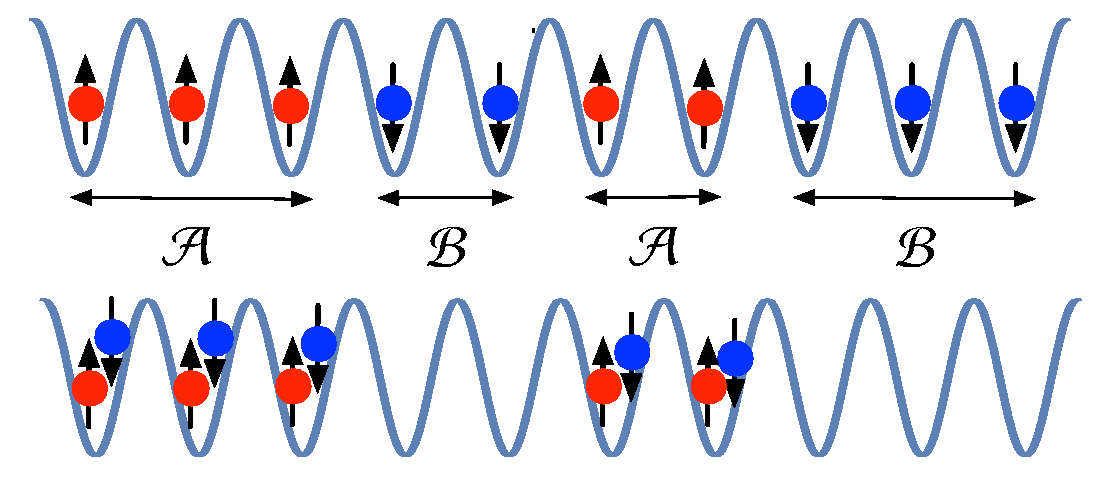
\includegraphics[width=1.0\columnwidth]{diffusion/schematic}
\caption{CDW 和 SDW 态的示意图。上栏为自旋密度波 SDW 的例子。下栏为电荷密度波 CDW 的例子。(取自\inlinecite{diffusion})}
\label{fig:diffusion:schematic}
\end{figure}

将上述三个引理结合起来,并利用我们在 \ref{sec:dynsymm} 节证明的受对称性保护的动力学对称性(定理 \ref{thm:dynsymm}),我们可以证明在半填充的二分 Fermi Hubbard 模型中,局域电荷密度和局域自旋密度之间存在严格映射,其期望值存在精确关系。

\begin{theorem}\label{thm:diffusion}
在半填充的二分 Fermi Hubbard 模型中,局域电荷密度在电荷密度波态的演化下的期望值,与局域自旋密度在自旋密度波的演化下的期望值,之间存在严格的精确关系。即,
\begin{align}
\langle \hat{n}_i(t)\rangle_{\psi_1} = 1 - \langle \hat{S}_i(t)\rangle_{\psi_2}.
\end{align}
其中 $|\psi_1\rangle$ 和 $|\psi_2\rangle$ 分别出自 CDW 类 和 SDW 类。
\end{theorem}

\begin{figure}[!htb]
\centering
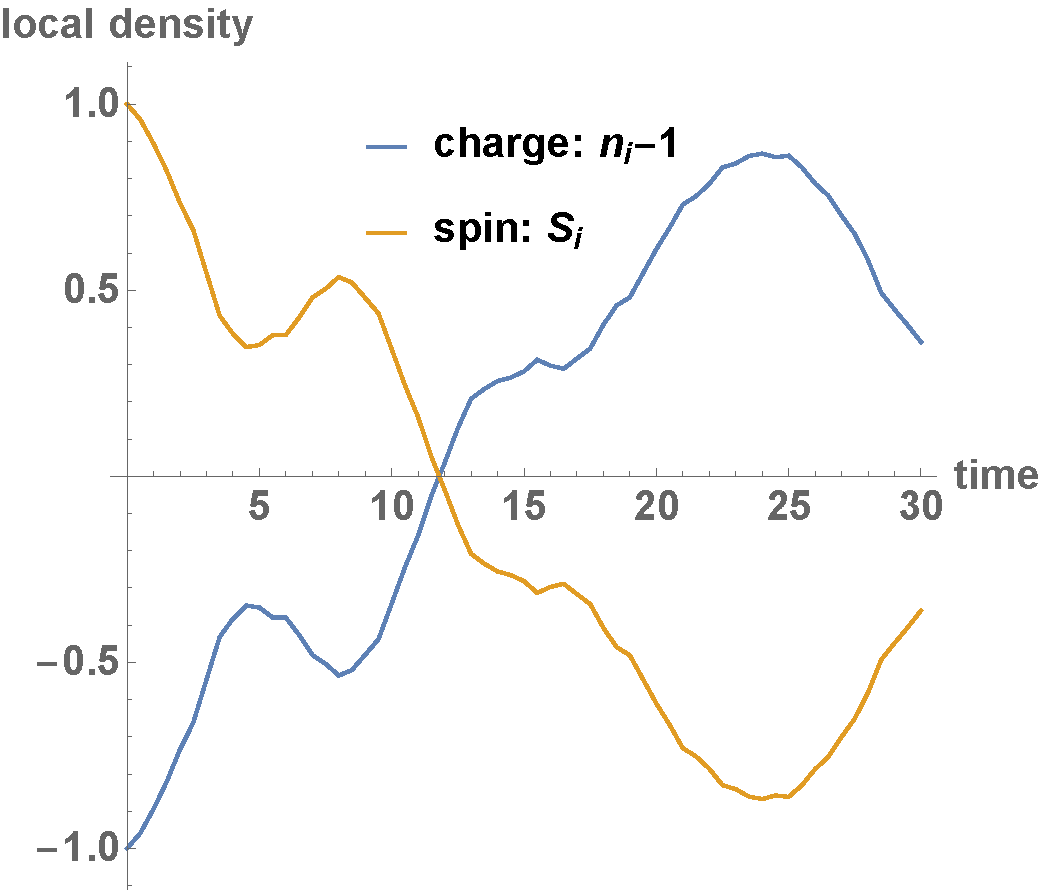
\includegraphics[width=0.7\columnwidth]{chap3_dynm/fhed}
\caption{Fermi Hubbard 严格对角化验证局域电荷密度与局域电荷密度的动力学演化。严格对角化在4个格点上进行,模型参数 $U/J=10$。取 $i=3$ 的格点进行测量。}
\label{fig:diffusion:fhed}
\end{figure}

\begin{proof}
对于二分的晶格,存在幺正变换 $\hat{W}$,
\begin{align}
W\hat{c}_{i\sigma}W^{-1} = (-1)^i\hat{c}_{i\sigma}
\end{align}
和时间反演变换 $\hat{R}$,使得 $S=RW$ 满足定理 \ref{thm:dynsymm} 中的条件,即
\begin{align}
\{S, \hat{H}_0\} = 0\\
[S, \hat{H}_I]=0
\end{align}
并且,局域电荷密度算符和局域自旋密度算符均具有 $S$-对称性,上面定义的 CDW 态 和 SDW 态均是 $S$-不变的。因此,利用上面三个引理,可得
\begin{align}
\langle \hat{n}_i(t)\rangle_{\psi_1, +U} 
&= \langle \psi_1|e^{iH(+U)t}\hat{n}_ie^{-iH(+U)t}|\psi_1\rangle \notag\\
&= \langle \psi_1|e^{iH(+U)t}\mathcal{P}^{-1}\mathcal{P}\hat{n}_i\mathcal{P}^{-1}\mathcal{P}e^{-iH(+U)t}|\psi_1\rangle \notag\\
&= \langle \psi_2|e^{iH(-U)t} (1-\hat{S}_i) e^{-iH(-U)t}|\psi_2\rangle \\
&= 1 - \langle \psi_2|e^{iH(-U)t} \hat{S}_i e^{-iH(-U)t}|\psi_2\rangle \notag\\
&= 1 - \langle \hat{S}_i(t) \rangle_{\psi_2, -U}, \notag 
\end{align}
再利用定理 \ref{thm:dynsymm},可得
\begin{align}
\langle \hat{S}_i(t)\rangle_{\psi_2, -U} = \langle \hat{S}_i(t)\rangle_{\psi_2, +U},  
\end{align}
因此有
\begin{align}\label{eq:n=1-S}
\langle \hat{n}_i(t)\rangle_{\psi_1, +U} = 1 - \langle \hat{S}_i(t)\rangle_{\psi_2, +U}. 
\end{align}
证毕。
\end{proof}

对于定理 \ref{thm:diffusion},我们进行了严格对角化的数值验证,见图 \ref{fig:diffusion:fhed}。



\subsection{偏离半满和更一般的观测量的推广}
上面为了叙述与证明的简便,假设了体系处于半满,并且只考虑了局域电荷密度观测量和局域自旋密度观测量的动力学演化行为。事实上,上述定理的半填充的约束完全可以放开,对观测量的定义也可以更广泛。。在文章\inlinecite{diffusion} 中,我们对定理做了更一般的表述。而证明的步骤仍是利用粒子空穴变换+受对称性保护的动力学对称性两步走。参考图 \ref{fig:diffusion:results} 的证明示意图。
\begin{figure}[!htb]
\centering
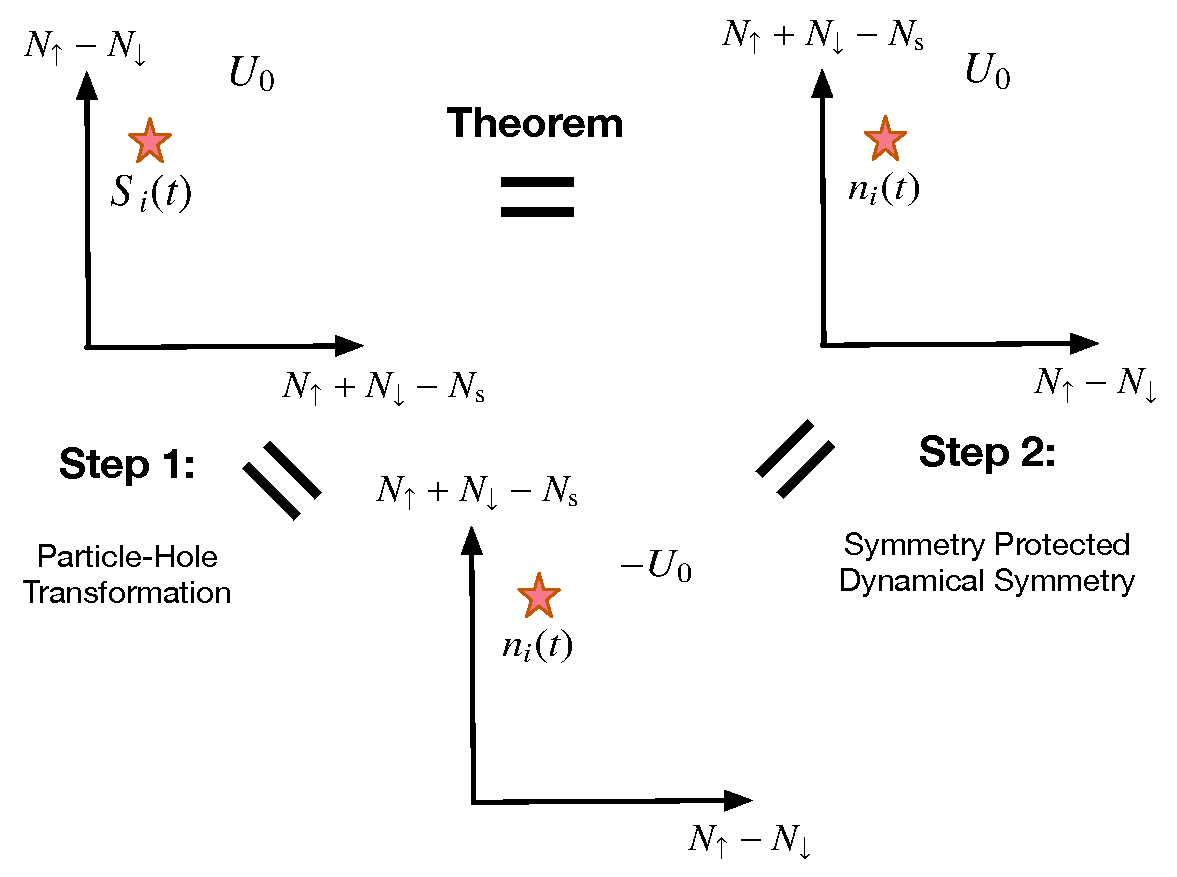
\includegraphics[width=1.0\columnwidth]{diffusion/results}
\caption{定理 \ref{thm:diffusion} 的证明示意图。 定理的证明分为两步:第一步是利用粒子空穴变换将$+U$的模型映射到$-U$的模型,同时将局域自旋密度量和局域电荷密度量进行映射;第二步是利用定理 \ref{thm:dynsymm} 中的受对称性保护的动力学对称性,将 $-U$ 的模型映射回 $+U$ 的模型,而同时特定可观测算符在特定初态下的动力学演化过程也被映射过来。(取自\inlinecite{diffusion})}
\label{fig:diffusion:results}
\end{figure}

对于更一般的情况,可观测量不再局限于局域电荷密度算符和局域自旋密度算符,凡是满足定理 \ref{thm:dynsymm} 所述,具有 $S$-对称性的算符均有类似的精确关系存在。对于态的定义也不局限于半填充,甚至不局限于定义\ref{def:state12}中的两类 CDW 和 SDW。凡是具有能相互映射的 $S_i$ 与 $1-n_i$ 的期望值的两个态均可以。


\subsection{温度效应}
还有一种推广是考虑温度的效应。当系统处于有限温时,体系不再是纯态。上面对态的讨论需改为对密度矩阵 $\rho=e^{-\beta H}$ 的讨论,这里 $\beta=1/T$,$T$ 是系统的温度。这种情况下可观测量的期望值为 
\begin{align}
n = tr(\rho\hat{n})
\end{align}
如果我们要证明局域电荷密度的动力学过程与局域自旋密度的动力学过程之间存在对称性,那我们就需要从上述密度算符 $\rho$ 和期望值 $n$ 出发进行证明,这不是一件容易的事情,甚至可能无法证明(而且很可能并不存在严格的对称性了)。然而,有一种特殊的情况我们可以严格证明定理仍然成立,那就是无穷高温的情况。一方面
\begin{align}
\mathcal{P}e^{-\beta H(+U)}\mathcal{P}^{-1} = e^{-\beta H(-U)}
\end{align}
另一方面,
\begin{align}
Se^{-\beta H(-U)}S^{-1} = e^{\beta H(+U)}
\end{align}
两者的联合变换使得
\begin{align}
\mathcal{P}S: e^{-\beta H} \leftrightarrow e^{\beta H}
\end{align}
无穷高温时,$\beta=0$,因此有
\begin{align}
e^{-\beta H} = e^{\beta H}
\end{align}
因此,在 $\mathcal{P}$ 和 $S$ 的联合变换下,无穷高温的混态系综 $\rho$ 被影射为它自己。而定理其他部分证明不变。因此对于无穷高温的情况,定理依然成立,局域电荷密度的动力学过程和局域自旋密度的动力学过程之间仍然可以相互映射。



\subsection{输运方程的对称性}
考虑局域密度观测量的扩散过程。
\begin{align}
    \partial_tn + \nabla\cdot\vec{j} = 0, \\
    \vec{j} = -D_c\nabla n. 
\end{align}
这里 $\vec{j}$ 是局域的流。从上式可推出扩散方程,
\begin{align}
    \partial_tn-D_c\nabla^2n = 0 
\end{align}
对于特定满足条件的初态,根据 (\ref{eq:n=1-S}) 式,则有
\begin{align}
    \partial_t\langle\hat{n}_i(t)\rangle_{\psi_1, +U} &= -\partial_t\langle\hat{S}_i(t)\rangle_{\psi_2, +U} \\ 
    \nabla^2\langle\hat{n}_i(t)\rangle_{\psi_1, +U} &= -\nabla^2\langle\hat{S}_i(t)\rangle_{\psi_2, +U}
\end{align}






\subsection{一类 Fermi-Hubbard 模型中的 SO(4) 对称性与电子-空穴对称性}\label{sec:so4}

在这里我们来讨论一类 Fermi Hubbard 模型所具有的 SO(4) 对称性\cite{yang1990}与电子空穴对称性。Fermi Hubbard 模型具有 SO(4) 对称性最早由杨振宁先生和张首晟教授在 \inlinecite{yang1990} 文章中予以证明,现已成为 Hubbard 模型研究领域的常识性的知识。事实上,通过 \ref{sec:diffusion} 上面提到的粒子空穴变换,即 
\begin{align}
    \mathcal{P} : \  \  
    & \hat{c}_{i\uparrow} \rightarrow (-1)^{i} \hat{c}_{i\uparrow}^{\dagger},  \nonumber\\
    & \hat{c}_{i\downarrow} \rightarrow \hat{c}_{i\downarrow}. 
\end{align}
以及上面证明过的引理 \ref{lemma1}(即对半填充的模型,在该变换下 $+U$ 的模型被映射为 $-U$ 的模型,反之亦然),很容易证明对于半填充的情况,该模型具有 $SO(4)$ 对称性。
首先,Fermi Hubbard 模型具有自旋-SU(2) 对称性,而上述映射将该 SU(2) 映射为 电荷-SU(2),因此同一个模型具有 SU(2)$\times$SU(2)=SO(4) 的对称性。

% 不过,半填充的约束在此处仍非必要。体系半填充就像体系是自旋平衡的一样,都是对于态的约束,这样的约束在讨论模型(哈密顿量)的对称性时完全可以放开。就像本节开头提到的,半填充只是调节化学势 $\mu$ 到 $\mu=N/2$ 的另一种表述,这样的常数项本身并不影响模型的对称性。作为更一般的情况,我们这里将该 SO(4) 对称性进行更普适地形式化表述。

% Fermi Hubbard 模型哈密顿量写作
% \begin{align}
%     \hat{H} = \sum_{\langle i,j\rangle,\sigma} -t\hat{c}_{i\sigma}^{\dagger}\hat{c}_{j\sigma} + \sum_{i} U \hat{n}_{i\uparrow}\hat{n}_{i\downarrow} 
% \end{align}

更严格的,对于半填充 Fermi Hubbard 模型,
\begin{align}
    \hat{H} = \sum_{\langle i,j\rangle,\sigma} -t\hat{c}_{i\sigma}^{\dagger}\hat{c}_{j\sigma} + \sum_{i} U \left(\hat{n}_{i\uparrow}-\dfrac{1}{2}\right)\left(\hat{n}_{i\downarrow}-\frac{1}{2}\right) 
\end{align}
可验证其具有如下定义的自旋SU(2)对称性和电荷SU(2)对称性。

\begin{definition}\label{def:spinsu2}
自旋$su(2)$生成元定义如下
\begin{align}\label{eq:spinsu2}
    \hat{S}_z &= \frac{1}{2}\sum_{i}\hat{c}_{i\uparrow}^{\dagger}\hat{c}_{i\uparrow}-\hat{c}_{i\downarrow}\hat{c}_{i\downarrow}, \\  
    \hat{S}_{+} &= \sum_{i}\hat{c}_{i\uparrow}^{\dagger}\hat{c}_{i\downarrow}, 
\end{align}
\begin{align}
    \hat{S}_{-} = \hat{S}_{+}^{\dagger}, \  \  
    \hat{S}_{x} = \frac{\hat{S}_{+}+\hat{S}_{-}}{2}, \  \  
    \hat{S}_{y} = \frac{\hat{S}_{+}-\hat{S}_{-}}{2i},
\end{align}
\end{definition}
容易验证,
\begin{align}
[\hat{H}, \hat{S}_{\alpha}]=0, \quad \alpha=x,y,z
\end{align}

\begin{definition}\label{def:spinsu2}
电荷$su(2)$生成元定义如下
\begin{align}
    \hat{L}_z &= -\frac{1}{2}\sum_{i}\hat{c}_{i\uparrow}^{\dagger}\hat{c}_{i\uparrow}+\hat{c}_{i\downarrow}^{\dagger}\hat{c}_{i\downarrow}+\frac{1}{2}N, \\ 
    \hat{L}_{+} &= \sum_{i}(-1)^i\hat{c}_{i\uparrow}\hat{c}_{i\downarrow} = \sum_{i}\exp(i\mathbf{Q}\cdot\mathbf{x}_i)\hat{c}_{i\uparrow}\hat{c}_{i\downarrow}
\end{align}
这里 $\mathbf{Q} = (\pi, \pi)$, $N$ 是总格点数,
\begin{align}
    \hat{L}_{-} = \hat{L}_{+}^{\dagger}, \  \  
    \hat{L}_{x} = \frac{\hat{L}_{+}+\hat{L}_{-}}{2}, \  \  
    \hat{L}_{y} = \frac{\hat{L}_{-}-\hat{L}_{-}}{2i}. 
\end{align}
\end{definition}
容易验证,
\begin{align}
[\hat{H}, \hat{L}_{\alpha}]=0, \quad \alpha=x,y,z
\end{align}

偏离半满时,$\mu\neq N/2$,容易验证,
\begin{align}
[\hat{H}, \hat{S}_{\alpha}] &= 0, \quad \alpha=x,y,z
\end{align}
仍成立,而且
\begin{align}
[\hat{H}, \hat{L}_{z}] &= 0 
\end{align}
但
\begin{align}
[\hat{H}, \hat{L}_{\pm}] &\neq 0 
\end{align}
即,此时模型仍具有自旋-SU(2)对称性,但不再具有电荷-SU(2)对称性。
事实上,这样的情况可以映射为 $U$ 相反的模型下加磁场的情况,即在模型中加入下面一项
\begin{align}
h\sum_{j}\hat{c}_{j\uparrow}^{\dagger}\hat{c}_{j\uparrow} - \hat{c}_{j\downarrow}^{\dagger}\hat{c}_{j\downarrow}
\end{align}
这种情况下,$S_x, S_y$ 仍是简并的,但二者不再与 $S_z$ 简并\footnote{若出现自旋密度波的话,序参量沿 $S_z$ 方向能量更低。}。对应到到电荷这边就是 (inplane) $L_{\pm}$ 不再与 $L_z$ 简并。在实验中,人们也观测到了这种情况下的 canted 序\cite{canted}。


另外,半填充的 Fermi Hubbard 模型还具有粒子空穴对称性。粒子空穴变换定义如下
\begin{align}
\hat{C}: \hat{c}_{i\sigma} \rightarrow (-1)^i\hat{c}_{i\sigma}^{\dagger}
\end{align}
容易验证,$[\hat{H}, \hat{C}]=0$。



除了通常的 Fermi Hubbard 模型,还有一些推广的 Fermi Hubbard 模型也具有上述两个对称性。这里,作为一个例子,我们来讨论如下的有效模型,该模型将在第 \ref{sec:floqhubb} 节中被更细致地讨论。
\begin{align}
\hat{H}_{\text{eff}} &= - \sum_{\langle i,j\rangle, \sigma} 
\left(J_0[(1-\hat{n}_{i\bar\sigma})(1-\hat{n}_{j\bar\sigma}) + \hat{n}_{i\bar\sigma}\hat{n}_{j\bar\sigma}]
+J_1[(-1)^l(1-\hat{n}_{i\bar\sigma})\hat{n}_{j\bar\sigma} + \hat{n}_{i\bar\sigma}(1-\hat{n}_{j\bar\sigma})]\right)
\hat{c}_{i\sigma}^{\dagger}\hat{c}_{j\sigma} \nonumber\\
& \quad + \tilde{U}\sum_{i}\left(\hat{n}_{i\uparrow}-\frac{1}{2}\right)\left(\hat{n}_{i\downarrow}-\frac{1}{2}\right)
\end{align}
% 对于 $J_0\neq J_1$ 的情况,
可以直接验证:

\begin{itemize}

\item $l$ 为偶数时,
\begin{align}
[\hat{H}_{\text{eff}}, \hat{S}_{\alpha}] &= 0, \quad \alpha=x,y,z \\
[\hat{H}_{\text{eff}}, \hat{L}_{\alpha}] &= 0, \quad \alpha=x,y,z 
\label{eq:HeffL}
\end{align}
因此模型具有 SO(4) 对称性。
\begin{align}
[\hat{H}_{\text{eff}}, \hat{C}]=0
\end{align}
因此模型具有粒子空穴对称性。

\item $l$ 为奇数时,
\begin{align}
[\hat{H}_{\text{eff}}, \hat{S}_{\alpha}] &= 0, \quad \alpha=x,y,z
\end{align}
因此模型具有 自旋-SU(2) 对称性,
但 (\ref{eq:HeffL}) 式不再成立,因此不具有 电荷-SU(2) 对称性。故而也不具有 SO(4) 对称性。

引入二分晶格变换 $\hat{S}$ (参考上一节内容),有
\begin{align}
[\hat{H}_{\text{eff}}, \hat{C}\hat{S}]=0
\end{align}
因此模型具有粒子空穴对称性。

\end{itemize}




\chapter{周期含时驱动的光晶格系统}

在这一章中,我们来讨论周期含时驱动的光晶格体系。首先,我们在


\section{周期含时驱动体系的 Floquet 理论} \label{sec:floqtheory}


\section{晃动光晶格}


\subsection{晃动光晶格中的拓扑物态}


\subsection{周期晃动光晶格实现 带有关联隧穿效应的 Fermi Hubbard 模型}


\section{关联隧穿效应诱导的铁磁态与相分离} \label{sec:floqhubb}
\chapter{拓扑物态的深度学习} \label{chap:topoml}

这一章,我们讨论拓扑物态的机器学习问题。首先,我们在第 \ref{sec:classify} 小节介绍拓扑物态分类的一般性理论,特别的,我们将介绍到一维 AIII 类的对称性约束与拓扑刻画,以及二维 A 类 和 D 类的对称性及拓扑刻画理论;在 \ref{sec:neuralnetwork} 节,我们介绍一种机器学习的算法,人造神经网络结构;在 \ref{sec:topoml} 我们讨论利用深度神经网络进行拓扑物态的机器学习问题,我们将介绍对于一维 AIII 类 四能带模型 的 绕数的学习,以及二维 A类 二能带模型的 Chern 数的学习。



\section{拓扑物态分类通论} \label{sec:classify}
在第 \ref{chap:chargepump} 章中,我们讨论了一类有能隙的费米子体系的绝热周期性演化,其绝热周期幺正的演化算符最终会与某类 一维系统上定义的 绕数(winding number)和二维参数空间上定义的陈数(Chern number)相联系。这些拓扑数表征了体系在某些方面的性质上具有量子化的整数平台,在前面的电荷输运的例子中,表现为系统每周期输运整数倍的电荷单位。这其实就是一个拓扑物态的例子。正如前文所述,拓扑物态的诸多良好性质,如鲁棒性、量子化平台等,吸引人们在过去几十年间对其进行了大量的研究。人们通过对大量特殊模型的研究,渐渐建立起了一套系统性的拓扑物态的分类理论\cite{topoclassify2016},下面进行介绍。

拓扑绝缘体讨论有能隙的无相互作用作用费米子体系。根据体系所具有的对称性的不同,可划分为一下十类:A,AIII,AI,BDI,D,DIII,AII,CII,C,和 CI 类。对于不同类(也就是不同对称性)的模型,可以用不同的拓扑数来刻画,其拓扑刻画的规律随着体系维度的变化而变化。对某一类维度和对称性的模型,其完整的拓扑刻画可能对应到例如 $\mathbb{Z}$,$2\mathbb{Z}$,或 $\mathbb{Z}_2$,甚至0。根据对称性的变化和模型维度的变化,人们建立起一个周期表(Periodic Table)来描述不同类别模型拓扑刻画的规则(叫\textit{周期表}是因为随着体系维度增加呈现出周期性结构),具体参考文献\inlinecite{topoclassify2016}。我们这里具体讨论两类,一维 AIII 类 和二维 A 类,这两类也是后面 \ref{sec:topoml} 节我们展开机器学习的类别。

在具体介绍 A 类 和 AIII 类之前,先让我们回顾第 \ref{chap:dynm} 章中提到的几种对称性变换。
\begin{itemize}
    \item 时间反演变换 $\mathcal{T}$:为反幺正变换,将 $\ii$ 映射为 $-\ii$
    \begin{align}
    \mathcal{T} \ii \mathcal{T}^{-1} \rightarrow \ii
    \end{align}

    \item 粒子空穴变换 $\mathcal{C}$:幺正变换,将费米子湮灭算符 $\psi$ 映射为产生算符 
    \begin{align}
        \mathcal{C}\psi\mathcal{C}^{-1} \rightarrow \psi^{\dag}
    \end{align}

    \item 手征变换,为时间反演变换和粒子空穴变换的结合,
    \footnote{在第 \ref{chap:dynm} 章中,时间反演算符和粒子空穴变换的记号分别为 $R$,$\mathcal{P}$,而 $S$ 用来指代时间反演变换和另一个幺正变换 $W$ 所结合的反幺正变换。}
    \begin{align}
        \mathcal{S} = \mathcal{T} \mathcal{C}
    \end{align}

\end{itemize}
根据是否具有这几种对称性,无相互作用的费米子体系被划分为上述10类。
其中,
A 类是一般的无特殊对称性约束的体系,只有在偶数维度的体系($d=2n$)中具有非平庸的拓扑分类,由 Chern 数刻画:
\begin{align}
C_n = \frac{1}{n!}\left(\frac{1}{2\pi}\right)^{n}\int\text{Tr} F^n
\end{align}
其中 
\begin{align}
F = dA - \ii A^2
\end{align}
$A$ 为被填充能带的 非阿贝尔联络,
定义如下
\begin{align}
A_i^{mn} = A_i^{mn}dk^i = \ii \langle u^m(\vect{k})|\partial_{\vect{k}_i} u^n(\vect{k})\rangle
\end{align}
类似于 第\ref{chap:chargepump} 章中 提到的非阿贝尔 Berry 联络,只是这里使用了微分的记号。$n=1$ 时就是由第一 Chern 数所刻画的二维模型,著名的例子如 Haldane 模型\cite{haldane1988} 就是一种 Chern 类绝缘体。对于这一 Chern 数,我们在附录 \ref{sec:chern} 中讨论了基于 \inlinecite{chern2005} 的算法,并证明了其相关性质。


而 AIII 类是只具有上述手征对称性($\mathcal{S}$)的体系。例如,第 \ref{chap:chargepump} 章中提到的 SSH 模型,即一维 AIII 类模型。由于手征对称性由粒子空穴对称性和时间反演对称性组合而成,粒子空穴对称性会将费米子产生算符映射为湮灭算符,因此,能谱须正负对称\footnote{迹不为0的情况相当于加了一常数矩阵,将其拿掉后还是正负对称},具有该对称性的哈密顿量矩阵 $\mathcal{H}(\vect{k})$,
\footnote{哈密顿量是 $H$,哈密顿量矩阵是 $\mathcal{H}(\vect{k})$}
\begin{align}
H(\vect{k}) = \psi_{\vect{k}}^{\dag}\mathcal{H}(\vect{k})\psi_{\vect{k}}
\end{align}
能找到幺正矩阵 $\mathcal{U}_S$ 与之反对易。
\begin{align}
\{\mathcal{U}_S, \mathcal{H}(\vect{k})\} = 0
\end{align}
以上要求保证了在 $\mathcal{U}_S$ 对角的基矢下,哈密顿量矩阵可写作如下块矩阵形式
\begin{align}
\mathcal{H}(\vect{k}) = \begin{pmatrix}
0 & D(\vect{k}) \\
D(\vect{k})^{\dagger} & 0
\end{pmatrix}
\end{align}
其中,$D(\vect{k})$ 幺正。
例如,这里再次举 SSH 的例子。SSH 哈密顿量在时空间写作
\begin{align}
H = -\sum_jt_1a^{\dagger}_{j}b_{j} + t_2 b^{\dagger}_ja^{j+1} + \text{H.c.}
\end{align}
变换到 $\vect{k}$-空间,哈密顿量写作
\begin{align}
H = \sum_{\vect{k}}
\begin{pmatrix}
a_{\vect{k}}^{\dag} & b_{\vect{k}}^{\dag}
\end{pmatrix}
\begin{pmatrix}
0 & t_1 + t_2e^{-\ii\vect{k}} \\
t_1 + t_2e^{\ii\vect{k}} & 0
\end{pmatrix}
\begin{pmatrix}
a_{\vect{k}} \\ b_{\vect{k}}
\end{pmatrix}
\end{align}
哈密顿量矩阵为
\begin{align}
\mathcal{H}(\vect{k}) = 
\begin{pmatrix}
0 & t_1 + t_2e^{-\ii\vect{k}} \\
t_1 + t_2e^{\ii\vect{k}} & 0
\end{pmatrix}
\end{align}
而这里找到的幺正矩阵为 $\hat{\mathcal{U}}_S = \sum_{\vect{k}} a^{\dag}_{\vect{k}}a_{\vect{k}} - b^{\dag}_{\vect{k}}b_{\vect{k}} $,
\begin{align}
\mathcal{U}_S = \begin{pmatrix}
1 & 0 \\
0 & -1 
\end{pmatrix} 
= \sigma_z
\end{align}
由于有上述形式的约束,对 AIII 类的刻画等价于对 $D(\vect{k})$ 的刻画。人们发现,只有在奇数维度的体系($d=2n+1$)才存在非平庸的拓扑分类,由绕数刻画,
\begin{align}
v_n = \dfrac{(-1)^nn!}{(2n+1)!}\left(\dfrac{\ii}{2\pi}\right)^{n+1}
\int\text{Tr}[(D^{-1}dD)^{2n+1}]
\end{align}
$d=1$, $n=0$ 时为一维的例子,由
\begin{align}
v_1 = \frac{\ii}{2\pi}\int_{\text{BZ}}\text{Tr}[D^{-1}dD]
\end{align}
刻画。例如上面提到的 SSH 模型,$t_1>t_2$ 时 $v_1=0$,$t_1<t_2$ 时 $v_1=1$。



\section{神经网络算法简介} \label{sec:neuralnetwork}
神经网络的算法结构经由 Geoffrey Hinton 等人的发展现在已经是机器学习中常用的成熟算法。神经网络在选择合适的激活元的情况下可以进行逆向传播
\footnote{逆向传播,backpropagation,其数学最早由 Yann LeCun 证明}
的过程,因此可以进行从\textit{学习}。
特别是后来 Geoffrey Hinton 等人提出 Dropout 等方法,使该算法在许多特定的任务上表现出色,例如 ImageNet 做图像识别\cite{imagenet2012}。对该算法的详细的讨论可参见\cite{prmlbook}。这里不再赘述。这里只对两种特殊的神经结构做描述,一种是全连接神经网络层,一种是卷积神经网络层\footnote{也由 Yann LeCun 最早提出}。

\begin{figure}[t]
\centering
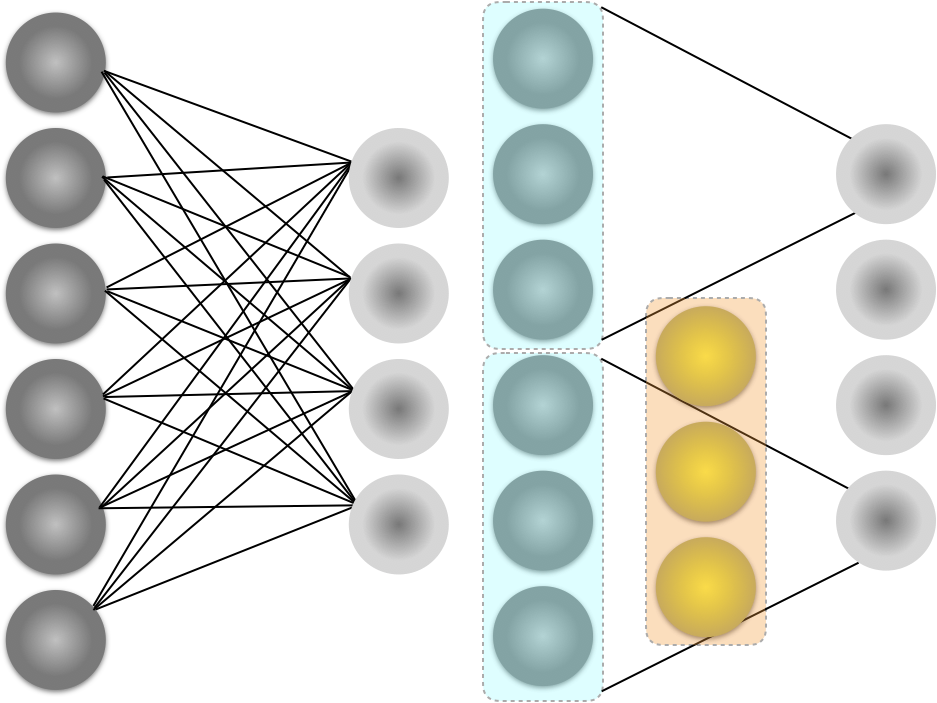
\includegraphics[width=1.0\columnwidth]{chap5_topoml/neuralnetwork}
\caption{神经网络层示意图。左:全连接神经网络层。右:卷积神经网络层,中间的黄色块表示卷积核。}
\label{fig:nn}
\end{figure}


\subsection{全连接神经网络}
全连接神经网络层的结构如图 \ref{fig:nn}(左) 所示。其数学定义如下:
\begin{align}
y_i = (f_{\text{F.C.}}(\vecr{x}))_i = f(a_{ij}x_j + b_i)
\end{align}
这里的 $\vecr{x}$ 对应图中左栏的输入,$x_j$ 是左栏输入中的第 $j$ 个元素,$y_i$ 对应右栏的输出中的第 $i$ 元素。这其实就是一个线性变换,图中从左栏连接右栏的一组实线代表了该线性变换的矩阵。$f$ 函数是一个非线性函数
\footnote{$f$ 是非线性函数非常重要,否则一系列线性变换接起来还是线性变换,将无法拟合非线性函数。}
,也叫激活元,一般取 sigmoid 函数或 ReLU 函数或其变形 \cite{prmlbook,topoml} ,sigmoid 函数也就是 tanh 函数,ReLU 函数定义如下
\begin{align}
f(x) = \begin{cases}
0, & x\leq0 \\
x, & x>0
\end{cases}
\end{align}

一系列全连接神经网络层相接得到的神经网络结构为
\begin{align}
f_{\text{F.C.}}^n\circ f_{\text{F.C.}}^{n-1}\circ \cdot f_{\text{F.C.}}^1\circ(\vecr{x})
\end{align}
其中引入了如下定义
\begin{align}
f_{\text{F.C.}}^{n}\circ f_{\text{F.C.}}^{n-1}(\vecr{x})
= f(a^{n}_{ij}[f(a^{n-1}_{jk}x_k + b^{n-1}_j)]_{j} + b^n_i)
\end{align}

这就是全连接神经网络层的构造方式,全连接(Fully-Connected)的含义就是输入层的每一个元素都连接到输出层的每一个元素,通过线性变换和非线性变换。




\subsection{卷积神经网络}
卷积神经网络层的结构如图 \ref{fig:nn}(右) 所示。其构造方式如下,
\begin{align}
y_i = (f_{\text{Conv.}}(\vecr{x}))_i = f(\sum_j^{d}k_jx_{i+j}+b_j)
\end{align}
$\vecr{k}$ 为长度为 $d$ 的卷积核,因此输入层的长度与输出层的长度相差 $d-1$。
\begin{align}
dim(\vecr{x}) - dim(\vecr{y}) = dim(\vecr{k}) - 1
\end{align}
例如,图 \ref{fig:nn}(右) 中所示的卷积层,左栏输入为 6 个元素,右栏输出为4 个元素,卷积核为 3个元素。卷积核与输入栏元素从上至下依次做 \textit{块}线性变换,然后作用非线性函数 $f$ 得到右边输出栏的相应元素。

在卷积神经网络层中,输入栏的元素不再“连接”至每一个输出栏的元素,而是由一个引入的卷积核(Kernel),依次块作用在输入栏上,将某一块的几个输入选素做线性变换,再做非线性变换,得到输出元素,卷积(Convolution)的意思也就在于此。

许多卷积神经网络层相连可以构造一个巨大的卷积神经网络层。但这并不是无限的,卷积层会缩小元素维度,这也正是其对数据进行\textit{降维}的体现——通过不断提取每一块离散像素中的有效信息(或说特征,Feature),抛却无效信息,渐渐学会识别一个东西。需要注意的是,全联接神经网络并不见得需要输入层比输出层大或输出层比输入层大。事实上,卷积神经网络层和全联接神经网络层可以相互连接,构造巨大的神经网络结构,以完成特定任务的有效学习。




\section{深度神经网络学习拓扑物态} \label{sec:topoml}
在这一节,我们讨论对拓扑物态的深度学习问题。在之前张鹏飞等人的工作中\inlinecite{zpf2017},他们发现了利用神经网络能够学习两能带的一维 AIII 类拓扑分类问题,其中卷积神经网络表现更好。这与卷积神经网络和基奇效学习的物理规律都具有平移不变性有着密切关系。两能带的一维模型相对来说输入的数据较少,浅层网络就可以承担学习任务。而对于更复杂的模型以及二维的模型,输入数据更为庞大,而其要学习的物理规律也相对更为复杂,这时浅层网络已无法完成学习任务
\footnote{经试验,浅层网络在几百次试验中均不能表现很好。我们没有做更多试验,转而寻求了深度神经网络。},深度学习的应用将必不可少。


我们利用深度卷积神经网络进行了两类拓扑物态的学习,一类是 一维的 AIII 类的四能带的模型,另一类是 二维 A 类的二能带模型。下面将做分别介绍。

\begin{figure}[t]
\centering
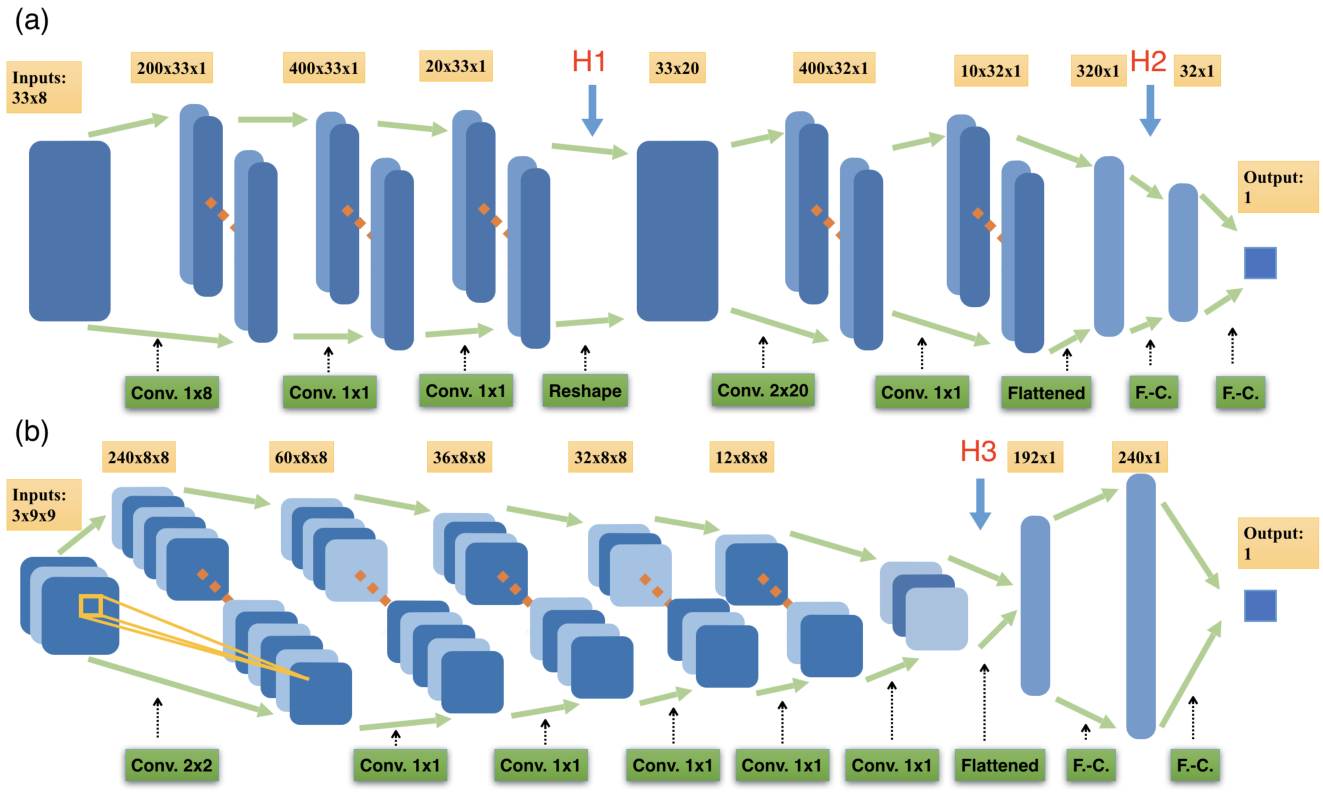
\includegraphics[width=1.0\columnwidth]{topoml/architecture}
\caption{深度学习拓扑物态网络结构示意图。(a) 训练学习一维 AIII 类绕数的网络结构;(b) 训练学习二维 A 类 Chern 数的网络结构。网络结构左侧为输入数据,右侧为输出标签。图中每一列上面标注了该层网络的神经元数目,其中左侧第一栏为输入数据的大小。层与层之间的箭头下方标注了该连接为全连接(Fully-Connected,F.-C.)还是卷积连接(Convolution,Conv.)。其中,卷积连接的方式标注了卷积核(kernel)的数目。(a) 中的两个箭头所指的地方,H1 和 H2,以及 (b) 中箭头所指的地方,H3,标注了三个隐藏层,这些隐藏层在机器训练好后被发现提取到了拓扑物态全局的关键信息。其中 (a) 中的隐藏层 H1 和 H2 提取到了\textit{转角} (winding angle)的特征(见图\ref{fig:anal-winding}),(a) 中的隐藏层 H3 被发现提取到了 \textit{固体角}(solid angle),也即 Berry 曲率的特征(见图\ref{fig:anal-chern})。这对理解机器学习方法的黑匣子,与理解机器经过训练之后有推广的预言能力来说至关重要。(取自\inlinecite{topoml})}
\label{fig:architecture}
\end{figure}




\subsection{一维 AIII 类 绕数的学习}
这一小节我们讨论一维 AIII 类拓扑类的机器学习问题。由 \ref{sec:classify} 节所述,哈密顿量矩阵为
\begin{align}\label{eq:D(k)}
    H(k)=\begin{pmatrix} 0 & D(k) \\ D^{\dagger}(k) & 0 \end{pmatrix}.
\end{align}
其中 $k$ 为U(1) 的参数。不失一般性地,我们这里选择 $D(k)$ 为幺正矩阵\footnote{平带近似不影响拓扑数,只要保持能隙不关闭就好。下同。}。由 \ref{sec:classify} 所述,这一类模型的拓扑由如下定义的绕数所刻画
\begin{align}
    w=\frac{1}{2\pi}\int_{-\pi}^{\pi}dk\mathrm{Tr}[D^{-1}(k)i\partial_kD(k)]. \label{wd1}
\end{align}
这里,由于 $D(k)$ 为幺正矩阵,其可被对角化为
\begin{align}
D(k) = V^\dag(k)M(k)V(k)
\end{align}
其中 $M(k)$ 为对角矩阵,且矩阵元全部为模1的复数,$\{e^{-i\theta_1(k)}, e^{-i\theta_2(k)},...,e^{-i\theta_d(k)}\}$。事实上,$D(k)$ 总是可以被分解为
\begin{align}
D(k) = e^{-\ii\alpha(k)}\bar{D}(k)
\end{align}
其中 $\bar{D}(k)$ 为 SU(d) 矩阵,$d$ 为矩阵维度,而
\begin{align}
\alpha(k)=\sum_i\theta_i(k)/d\in [-\pi/d,\pi/d)
\end{align}
这样以来,绕数公式可以继续被简化,
\begin{align}\label{eq:wdalpha}
    w=\dfrac{1}{\pi}\int_{-\pi}^{\pi}dk\partial_k\alpha(k),
\end{align}
在我们的工作中\cite{topoml},我们考虑 $d=2$ 的情况。这种情况下有
\begin{align}
\alpha(k)=(\theta_1(k)+\theta_2(k))/2 \mod \pi
\end{align}
而
\begin{align}
\alpha(k)\in[-\pi/2,\pi/2)
\end{align}
因此,将参数 $k$ 做离散化后,上述绕数公式在离散化的版本下写作
\begin{align}
    w &=\dfrac{1}{\pi}\sum_{l=1}^{L}\Delta\alpha(k_l) \notag\\
        &=\dfrac{1}{\pi}\sum_{l=1}^{L}[\alpha(k_{l+1})-\alpha(k_l)]\mod \pi, \label{wd_dis}
\end{align}
这里 $ k_i $, $ i=1,\ldots,L $ 均匀分布在第一布里渊区,且有
\begin{align}
\Delta\alpha(k)\in[-\pi/2,\pi/2)
\end{align}

\begin{figure}[!htb]
\centering
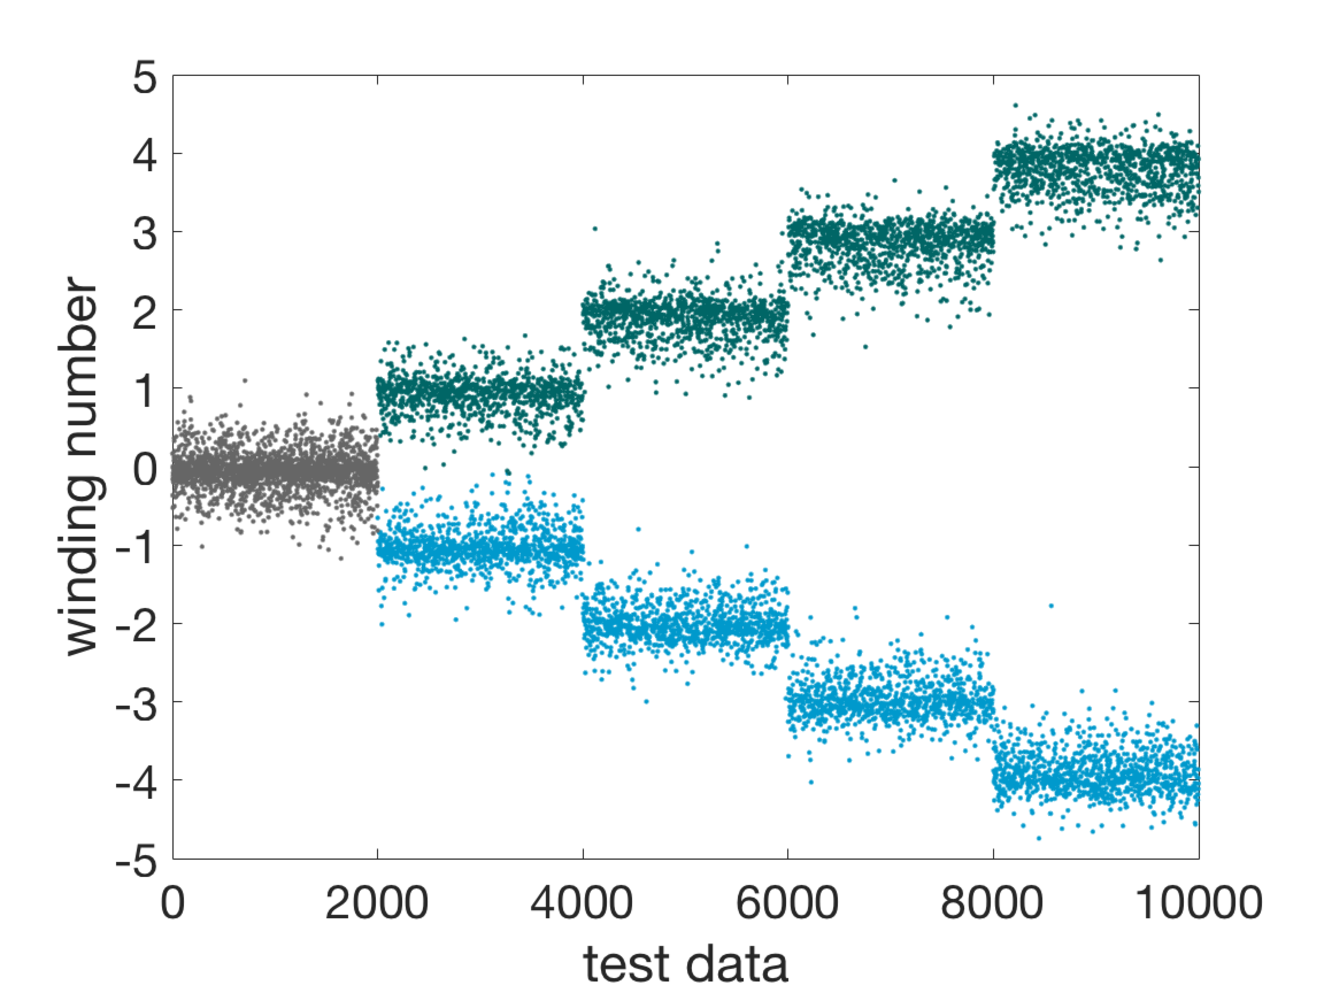
\includegraphics[width=1.0\columnwidth]{topoml/winding_performance}
\caption{一维绕数的测试表现结果。测试在10000组哈密顿量构型上进行,它们分别被标记为1到10000,即横坐标。注意,这里的标记并不是训练的标签,而是指图中的横坐标,图 \ref{fig:perf-chern} 中同此。
其中,从2000 i到2000(i+1)的哈密顿量具有$\pm i$的绕数,其中 $+$ 的以绿色标记,$-$的以青色标记。图中点的纵坐标即测试中机器所预言的结果(神经网络\ref{fig:architecture}(a)的输出)。(取自\inlinecite{topoml})}
\label{fig:perf-winding}
\end{figure}

我们对这一类模型的绕数进行了监督式学习,利用了深层的卷积神经网络,网络结构如图 \ref{fig:architecture} (a) 所示。
其用来训练的输入数据是哈密顿量构型,标签为模型的绕数。模型构型即如下矩阵
\begin{align}
    \begin{pmatrix}
        \Re[D_{11}(0)] & \Re[D_{11}(2\pi/L)] & \cdots & \Re[D_{11}(2\pi)] \\
        \Im[D_{11}(0)] & \Im[D_{11}(2\pi/L)] & \cdots & \Im[D_{11}(2\pi)] \\
        \Re[D_{12}(0)] & \Re[D_{12}(2\pi/L)] & \cdots & \Re[D_{12}(2\pi)] \\
        \Im[D_{12}(0)] & \Im[D_{12}(2\pi/L)] & \cdots & \Im[D_{12}(2\pi)] \\
        \Re[D_{21}(0)] & \Re[D_{21}(2\pi/L)] & \cdots & \Re[D_{21}(2\pi)] \\
        \Im[D_{21}(0)] & \Im[D_{21}(2\pi/L)] & \cdots & \Im[D_{21}(2\pi)] \\
        \Re[D_{22}(0)] & \Re[D_{22}(2\pi/L)] & \cdots & \Re[D_{22}(2\pi)] \\
        \Im[D_{22}(0)] & \Im[D_{22}(2\pi/L)] & \cdots & \Im[D_{22}(2\pi)]
    \end{pmatrix}
\end{align}
其中 $\Re$ 表示复数的实部,$\Im$ 表示复数的虚部。这是一个 $8\times L$ 的矩阵。当离散化到 $L=32$ 时,即 $8\times32$ 的矩阵,如图 \ref{fig:architecture}(a) 所示。
\footnote{图 \ref{fig:architecture}(a) 中 input 显示 $33\times8$,实际上是考虑了周期性边界条件,把第一列输入在最后一列后面复制了一遍。在下面的二维Chern数的例子里,也是如此。}

我们用 python TensorFlow 库 和 Wolfram Mathematica 写程序实现上述机器学习任务。训练集里的模型哈密顿量具有$\{0, \pm1, \pm2, \pm3\}$的绕数。经训练后的网络在测试集上的表现如表\ref{table:winding-sr}所示。
\footnote{具体训练和测试参数见我们的文章\inlinecite{topoml}。}
\begin{table}[t]
\caption{神经网络在测试集上的表现。对于绕数(w)分别为 $0, \pm1, \pm2, \pm3, \pm4$ 的测试哈密顿量,神经网络 \ref{fig:architecture} (a) 输出结果的精确度。 }\label{table:winding-sr}
\centering
% \begin{ruledtabular}
\begin{tabular}{*{8}c}
\hline\hline
& 绕数(w) & 0 & $\pm1$ & $\pm2$ & $\pm3$ & $\pm4$ & \\ \hline
& 精确度 & 97\% & 96\% & 96\% & 95\% & 93\% & \\
\hline\hline
\end{tabular}
% \end{ruledtabular}
\end{table}
其在测试集上的表现如图 \ref{fig:perf-winding} 所示。
可见,经训练后的神经网络在测试集上的测试结果具有很高精确度,对于已见过的类能以$>95\%$的精确度进行预言,甚至还可以以 $>90\%$ 的精确度预言绕数为 $\pm4$ 的类,具有一定程度的推广能力。




\begin{figure}[t]
\centering
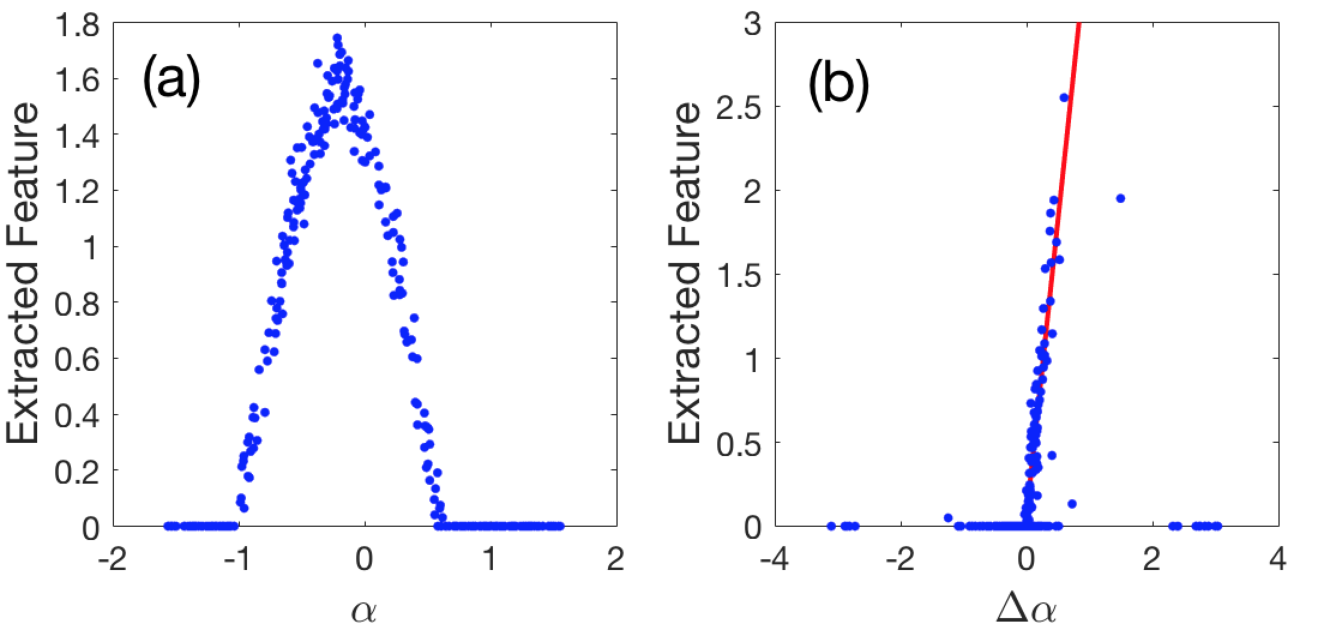
\includegraphics[width=1.0\columnwidth]{topoml/analysis_winding}
\caption{一维绕数学习的神经网络结构隐藏层分析。在机器完成训练后之后进行测试,打开神经网络\ref{fig:architecture}(a),其中的隐藏层H1 和 H2 的中间输出结果。(a) H1层的输出结果散点图,横坐标为测试模型的 $\alpha$ 角的真实值,而纵坐标为 H1 层 的输出结果,可见 H1 层实际上提取到了模型的 $\alpha$ 特征;(b) H2层输出结果的散点图,横坐标为测试模型的 $\Delta\alpha$ 的真实值,而纵坐标为 H2层的输出结果,可见 H2 层实际上提取到了模型的 $\Delta\alpha$ 特征。(取自\inlinecite{topoml})}
\label{fig:anal-winding}
\end{figure}



为理解神经网络进行绕数学习的黑盒子,以及理解其训练后具有推广能力的原因,我们尝试对训练后的神经网络结构进行解析。通过打开图 \ref{fig:architecture} (a) 中的网络,查看其隐藏层的输出,我们一定程度上理解了其学习机理。如图 \ref{fig:anal-winding} (a) 所示,通过画出 $\alpha$ 角和 H1 输出值的散点图,可以看出,H1 层实际上提取到了 $\alpha$ 角的有效特征。而如图 \ref{fig:anal-winding} (b) 所示,通过画出 $\Delta\alpha$ 和 H2 输出值的散点图,可以看出,H2 层实际上提取到了 $\Delta\alpha$ 的有效特征。而根据(\ref{eq:wdalpha})和(\ref{wd_dis})式,绕数实际上正是由 $\alpha$ 和 $\Delta\alpha$ 所计算出。这也就说明,机器通过学习体系全局的特征、学习物理的规律而学会了绕数,而不是蒙上的。这也正是其推广能力的来源。这在下面的 Chern 数的机器学习中也有体现。




\subsection{二维 A 类 陈数的学习}
这一小节我们讨论二维 A 类拓扑类的机器学习问题。由 \ref{sec:classify} 节所述,A 类没有对称性约束。在此我们考虑两能带模型,对这样的模型,哈密顿量矩阵可以一般地写为:
\begin{align}
    H(\mathbf{k})=\mathbf{h}(\mathbf{k})\cdot\boldsymbol{\sigma}=h_x(\mathbf{k})\sigma_x+h_y(\mathbf{k})\sigma_y+h_z(\mathbf{k})\sigma_z.
\end{align}
这里 $\boldsymbol{\sigma}=(\sigma_x,\sigma_y,\sigma_z)$ 是泡利矩阵矢量,和上一小节一样,我们取平带近似,这不影响其拓扑刻画。对于二维模型,其拓扑由下式 Chern 数刻画,
\begin{align}\label{eq:c1}
    C=\dfrac{1}{2\pi}\int_{T^2}d^2\mathbf{k}F_{xy}(\mathbf{k}), 
\end{align}
这里 $T^2$ 指第一布里渊区(Torus结构),而
\begin{align}%\label{eq:c1AF}
A_{\mu}(\mathbf{k}) &= i\langle u(\mathbf{k})|\partial_{\mu} u(\mathbf{k})\rangle, \\ 
F_{\mu\nu}(\mathbf{k}) &= \partial_{\mu}A_{\nu}-\partial_{\nu}A_{\mu}.
\end{align}

\begin{figure}[t]
\centering
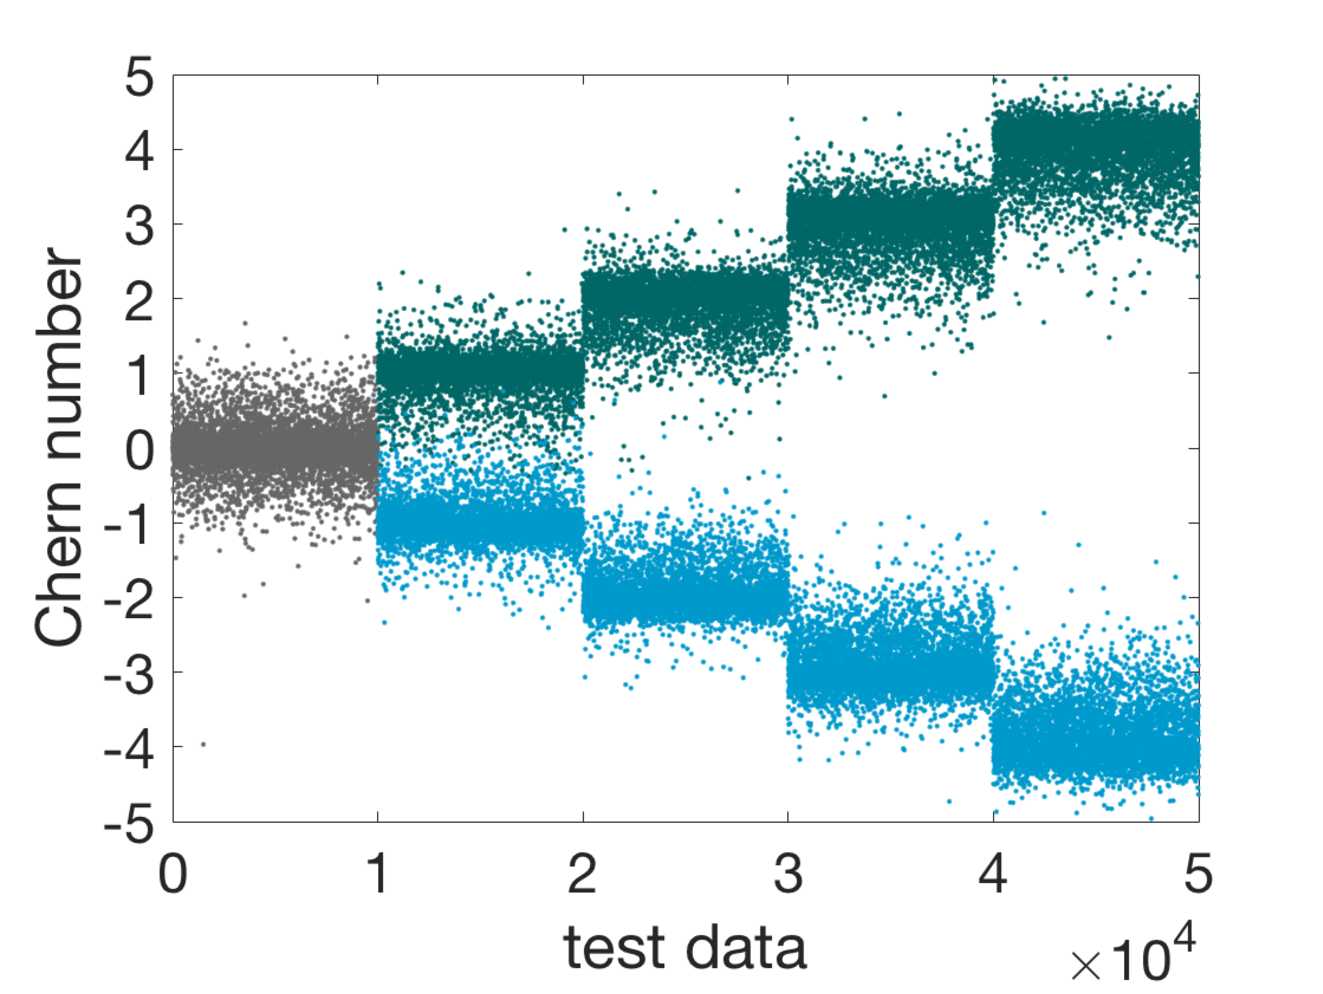
\includegraphics[width=1.0\columnwidth]{topoml/chern_performance}
\caption{二维Chern数的学习测试表现结果。测试在 $5\times10^4$ 组哈密顿量构型上进行,它们分别被标记为1到50000,即横坐标的值。其中,从10000i 到10000(i+1)的哈密顿量具有 $\pm i$ 的Chern 数,其中 $+$ 的以绿色标记,$-$的以青色标记。图中点的纵坐标即测试中机器所预言的结果(神经网络\ref{fig:architecture}(b)的输出)。(取自\inlinecite{topoml})}
\label{fig:perf-chern}
\end{figure}


我们利用深层神经网络对二维 A 类两能带模型的 Chern 数进行了机器学习,网络结构如图 \ref{fig:architecture} (b) 所示。
输入数据依然为哈密顿量构型,即 
\begin{align}
\begin{pmatrix}\mathcal{H}_x, & \mathcal{H}_y, & \mathcal{H}_z 
\end{pmatrix}
\end{align}
其中
\begin{align}
\mathcal{H}_{\mu} &=
\begin{pmatrix}
h_{\mu}(0,0) & h_{\mu}(0,\frac{2\pi}{L}) & \cdots & h_{\mu}(0,2\pi) \\
h_{\mu}(\frac{2\pi}{L},0) & h_{\mu}(\frac{2\pi}{L},\frac{2\pi}{L}) & \cdots & h_{\mu}(\frac{2\pi}{L},2\pi) \\
\vdots & \vdots & \ddots & \vdots \\
h_{\mu}(2\pi,0) & h_{\mu}(2\pi,\frac{2\pi}{L}) & \cdots & h_{\mu}(2\pi,2\pi) \\
\end{pmatrix}.
\end{align}
这里将 二维参数空间 $(k_x,k_y)$ 离散化为 $L\times L$ 个格点,模型的理论 Chern 数值可有附录 \ref{sec:chern} 中的算法计算。


我们用 Wolfram Mathematica 写程序实现上述机器学习任务。训练集里的模型哈密顿量 Chern 数有 $C\in\{0, \pm1, \pm2\}$,经训练后的网络在测试集上的表现如表\ref{table:winding-sr}所示。
\footnote{具体训练和测试参数见我们的文章\inlinecite{topoml}。}

\begin{table}[t]
\centering
\caption{神经网络在测试集上的表现。对于 Chern 数分别为 $0, \pm1, \pm2, \pm3, \pm4$ 的测试哈密顿量,神经网络 \ref{fig:architecture} (b) 输出结果的精确度。}
\label{table:chern-sr}
% \begin{ruledtabular}
\begin{tabular}{*{8}c}
\hline\hline
& $C$ & $0$ & $\pm1$ & $\pm2$ & $\pm3$ & $\pm4$ & \\ \hline
& Accuracy & 93\% & 92\% & 90\% & 86\% & 85\% & \\
\hline\hline
\end{tabular}
% \end{ruledtabular}
\end{table}

其在测试集上的表现如图 \ref{fig:perf-chern} 所示。
可见,经训练后的神经网络在测试集上的测试结果具有很高精确度,对于已见过的类能以$>90\%$的精确度进行预言,甚至还可以以 $>85\%$ 的精确度预言其没有见过的 Chern 数为 $\pm3,\pm4$ 的类,具有一定程度的推广预言能力。


\begin{figure}[!htb]
\centering
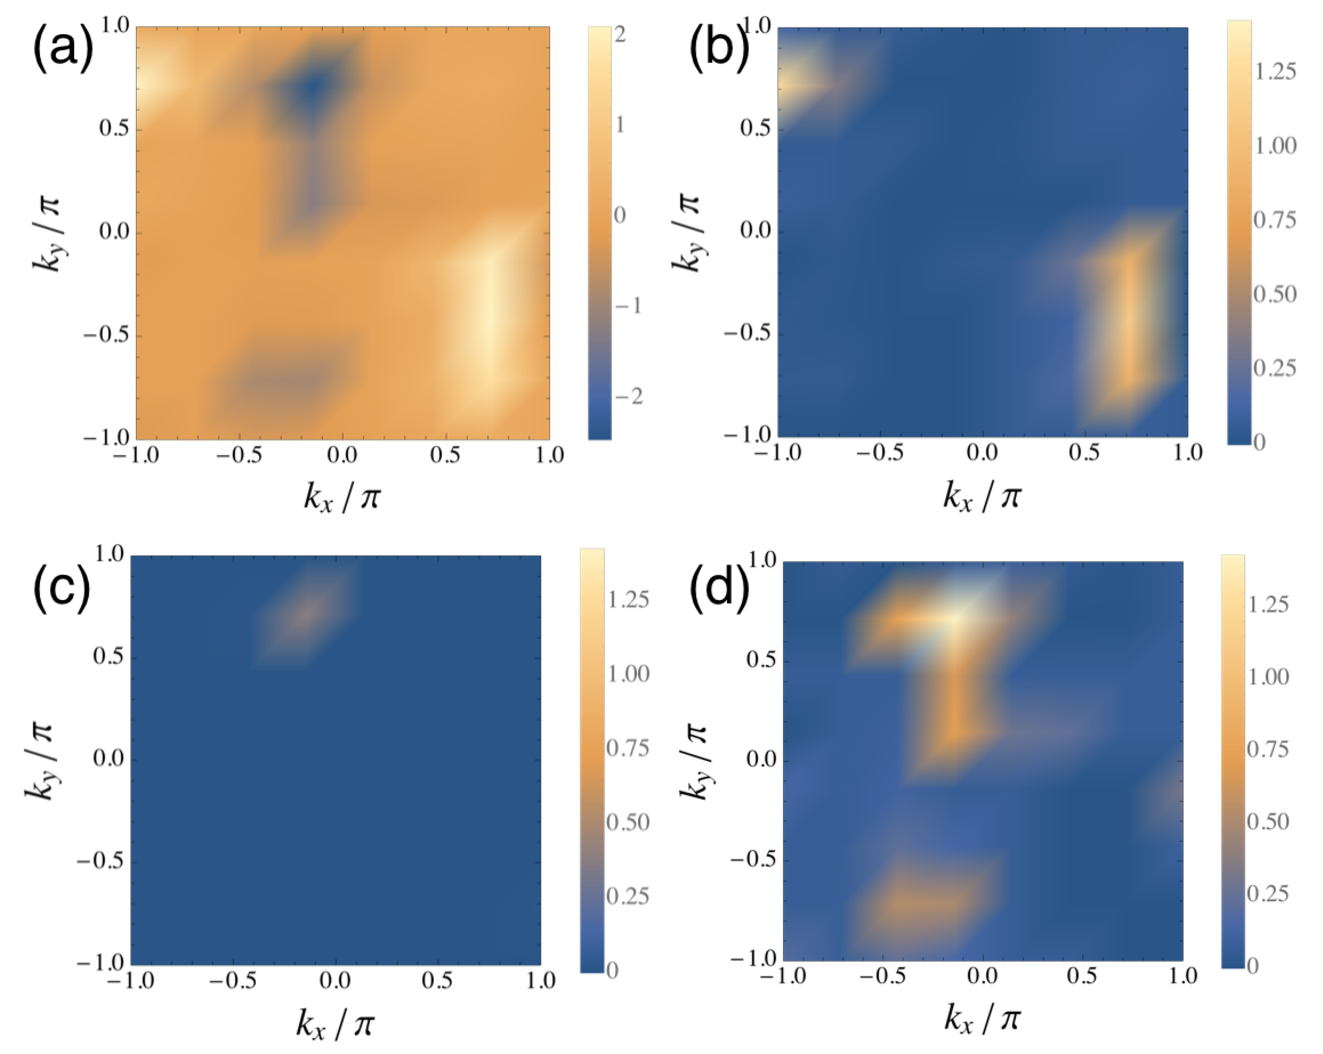
\includegraphics[width=1.0\columnwidth]{topoml/analysis_Berry}
\caption{二维Chern数学习的神经网络结构隐藏层分析。在机器完成训练之后进行测试,打开神经网络\ref{fig:architecture}(b),其中的隐藏层 H3 的中间输出结果。注意到,H3为三层的矩阵输出。(a) 测试模型的 Berry 曲率场真实值,由附录\ref{sec:chern} 中所述算法算得;对比图例可以看到,其中矩阵元有正有负。(b-d) H3 处三层矩阵的输出值;对比图例可以看出,输出值均为正值,且 (b) 层主要提取到了 (a) 中的正的部分,(d) 层主要提取到了 (a) 中的负的部分,而 (c) 层神经元几乎全部死掉(输出为0)。可见,H3 层实际上提取到了模型的 Berry 曲率场(也就是固体角)特征。(取自\inlinecite{topoml})}
\label{fig:anal-chern}
\end{figure}

为理解其学习机理和推广能力,我们将神经网络内层打开,尝试解析训练后的神经网络结构。如图 \ref{fig:architecture}(b) 所示,我们领网络在 H3 处输出其中间结果,对某一个典型的例子的输出结果如图 \ref{fig:anal-chern} 所示。其中,图 \ref{fig:anal-chern} (a) 为该模型的真实的 Berry 曲率场,而 (b-d) 为 H3 的输出结果。(a) 的值有正有负,而 (b-d) 均为正值,对比图例可知。这与神经网络中所取的激活元为 ReLU 函数有密切关系\cite{topoml}。由图还可看出,(c) 中的神经元大多死掉了,而 (b) 和 (d) 则通过分别提取 (a) 中正的部分和负的部分来提取到了 Berry 曲率场的全局特征。

由此可见,对神经网络进行拓扑数的训练使其学到了不止是拓扑数一个数字,而是包含了体系全局的和物理的特征在其中。我们在训练的时候,并没有告诉机器要去学习积分公式或者几何相角这样的局域信息,只是扔给它一个拓扑数的标签,而经过训练,机器自己学会了提取局域的几何特征和全局的拓扑特征。这也是其具有推广预言能力的来源。这使我们对机器的学习机理有了一定程度的理解。

这里需要补充说明的是,我们生成模型的方式是通过随机生成模型的傅立叶分量来构造大量的模型,这些模型构型随后被用于机器的训练或测试。这个过程中并没有检测这些模型是不是一定有能隙的,或者对于离散化的模型,其能隙可能是非常小,以致于 Berry 曲率会非常奇异。然而,无能隙的体系是不能算其 Chern 数的,对于离散化的情况,Berry 曲率过去奇异也会导致计算结果有偏差(见附录\ref{sec:chern}讨论)。事实上,这可能正是上述机器语言精确度没有达到很精确\footnote{很精确,例如99\%,99.9\%, 甚至更高}的原因之一。当然,这种偏差可以通过增加足够大的离散化来减小,而这又会使输入数据的维度大大增大,使机器训练的难度变大。当数据数据的维度增大很多时,网络结构本身可能就需要重新设计了。




\chapter{总结与展望}

本文详细讲述了作者在博士期间的主要研究工作。作者在读博期间进入超冷原子物理这个方兴未艾的领域,并对其中的超冷原子光晶格体系进行了一系列深入的研究,研究重点集中在其拓扑性质和含时动力学性质方面。本文详细论述了作者在这两方面的几个工作,下面分别进行总结。


\section{拓扑}

在拓扑方面:

1)作者和合作者们研究了光晶格中的拓扑电子输运问题,提出了 Creutz 梯上的拓扑电子泵模型,给出了该模型完整的拓扑相图,并提出了该模型中以偶数为内禀输运单位的绝热拓扑电荷输运过程;我们发现,在该模型中的各种拓扑电子输运路径和其相图上不同部分的 Zak 相角之间有密切关系;我们还通过数值模拟的方法对该模型的绝热拓扑输运过程进行了验证。
(见第 \ref{chap:chargepump} 章)

2)作者和合作者们使用了深度学习的方法,利用深层人工神经网络进行了拓扑物态的机器学习;我们对机器进行一维 AIII 类 和 二维 A 类拓扑物态的识别训练,利用绕数和Chern数作为训练标签,使之取得了超过90\%的预言精度,且结果具有推广性,能够以较高精度预言未见过的类别;我们打开深层神经网络,发现在其中间隐藏层提取到了全局的 Berry 曲率场的信息——也就是机器并不止学会了一个拓扑数,它通过学习全局知识学习到了拓扑物态的精髓,因此“学会”了分类拓扑相。
(见第 \ref{chap:topoml} 章)

3)作者为人们常用到的二维材料的陈数算法\cite{chern2005}开发了专门的基于 python3 语言 和 基于 Wolfram Mathematica 语言的程序包,并在本论文中证明了该算法的有效性与量子化、规范不变等性质(见附录 \ref{sec:chern})。





\section{动力学}

在含时动力学方面:

1)作者和合作者们证明了一类有 Hubbard 相互作用的体系中受单粒子对称性保护的动力学对称性,该定理能够将几个截然不同的实验现象\cite{hubbard-expan-2010,hubbard-expan-2012,mbl1d,twobody-2017}联系起来;作者和合作者们用严格对角化的数值方法对三类例子进行了检验;这三类例子分别联系着 Fermi Hubbard 扩散实验\inlinecite{hubbard-expan-2010,hubbard-expan-2012},玻色子带磁通的 Hubbard 模型上少体相互作用极限的实验\inlinecite{twobody-2017},和一维准无序多体局域化的实验\inlinecite{mbl1d}。
(见第\ref{chap:dynm} 章 \ref{sec:dynsymm} 节)

2)作者和合作者们证明了在二分 Fermi Hubbard 模型中电荷和自旋输运方面存在精确关系;作者在本论文中还讨论了该定理的推广、以及温度效应等。
(见第\ref{chap:dynm} 章 \ref{sec:diffusion})

3)作者和合作者们对周期含时驱动的 Floquet 系统进行了研究,并重点研究了
在近共振高频驱动的框架下的正方晶格 Fermi Hubbard 模型,该模型在蜂巢晶格中的实现在2018年由苏黎世联邦理工学院的实验小组报告\cite{correlated-tunnel-expr-2018-shaking}。利用标准路径积分平均场的方法,我们计算出了完整的平均场相图,并发现了在小的有效相互作用区域存在的铁磁相和相分离;这种铁磁相出现的机制完全是由于近共振的高频驱动以及由其引起的关联隧穿效应,有别于凝聚态中周知的 Stoner 机制。这种新奇的铁磁相有望在冷原子实验中被检验。
(见第\ref{chap:chargepump} 章)



\section{展望}

自从上世纪人类利用激光冷却和蒸发冷却的方法将稀薄的原子气体云冷却到百纳开尔文级别的低温,以及利用这样的低温实现了碱金属原子的玻色爱因斯坦凝聚\cite{bec1995a,bec1995b},人们对稀薄的超冷原子气体系统展开了一系列来自理论和实验的研究。近二十年时间以来,超冷原子物理领域的发展迅猛,研究成果愈加丰富。一方面,超冷原子气体体系有自己内在的丰富物理,例如少体物理问题,另一方面,人们利用超冷原子气体系统进行了一系列广泛关注的量子多体问题的研究,例如对一系列量子霍尔效应同源的物理系统与过程的研究\cite{topo2016zoller,harper1,harper2,zak-expr-2013,chern-expr-2015,ab-expr-2015,wilsonline-expr-2016,haldane-expr-2014,charge-pump-expr-2016-de,charge-pump-expr-2016-jp,4dqhall-expr-2018},对 Hubbard 模型的量子模拟\cite{hubbard-expan-2010,hubbard-expan-2012,microscope5,microscope6,af1,af2,af3,canted,incommensurate,af_long_range,pair_attractive,hidden_af_doped,charge-diffusion,spin-diffusion,floq-hubb-expr-2018,correlated-tunnel-expr-2018-shaking,correlated-tunnel-expr-2018-raman},对本征态热化假说\cite{thermalize-entropy-2016}与多体局域化\cite{mbl1d,mbl2d}等复杂问题的研究等。由于超冷原子系统的干净、可控,人们还可以研究一些传统凝聚态难以实现的系统与过程,例如周期驱动的体系\cite{haldane-expr-2014,floq-hubb-expr-2018,correlated-tunnel-expr-2018-shaking}与动力学淬灭过程。而利用诸如 Feshbach 共振等手段,体系的参数可以被在很大的范围内调控,这也大大拓宽了冷原子物理可以涉及的范围。

近来,超冷原子物理领域在探测手段和调控技术等方面取得了许多重要进展,例如量子气体显微镜的发展,这些进展使人们可以对强相互作用强关联体系的物理做更深入的研究与探测,例如单格点分辨、时间分辨的探测。人们已经利用这些喜人的成果实现了诸如一维 Luttinger 液体\cite{hidden_af_doped}、斜面反铁磁序\cite{canted}等物理。而这些不断的进展为超冷原子物理领域提供了丰富的方法和手段,和许多本身就丰富的物理。利用这些成果,人们未来有希望对许多强关联体系建立更深入的理解,有希望对更多诸如动力学淬灭的体系展开研究。例如作者博士期间和合作者们提出的近共振驱动的铁磁相\cite{floqhubb},有希望在未来的实验中加以验证。而超冷原子光晶格体系作为本领域尤为重要的领域和平台,未来有希望排上更大用场,甚至在诸如量子计算和量子信息方面发挥作用\cite{bloch2012}。

未来可期。




%%% 其它部分
\backmatter

%% 本科生要这几个索引,研究生不要。选择性留下。
% 插图索引
% \listoffigures
% 表格索引
% \listoftables
% 公式索引
% \listofequations


%% 参考文献
% 注意:至少需要引用一篇参考文献,否则下面两行可能引起编译错误。
% 如果不需要参考文献,请将下面两行删除或注释掉。
% 数字式引用
\bibliographystyle{thuthesis-numeric}
% 作者-年份式引用
% \bibliographystyle{thuthesis-author-year}
\bibliography{ref/refs}

%% 附录
\begin{appendix}
% % \newcommand{\vect}{\boldsymbol}
% \newcommand{\vect}{\mathbf}

\chapter{二维材料 Chern 数算法}\label{sec:chern}

考虑无限大二维材料的布里渊区(Brillioun Zone,简称BZ),其由两个实参数刻画,$\{k_x, k_y\}$,也即准动量$\vect{k}=(k_x, k_y)$。参数空间为 Torus 结构 (以下简称$T^2$),即 $k_x\in[0, 2\pi]$, $k_y\in[0, 2\pi]$,且 0 与 $2\pi$ 等价。考虑该材料的某一能带,引入其波函数记作 $|u(\vect{k})\rangle$,则陈数(以下称 Chern 数)刻画了一个从该 Brillioun 区($T^2$)上的到一个球面(以下简称$S^2$)的映射:

\begin{align}
T^2 \rightarrow S^2 : C = \frac{1}{2\pi}\int_{T^2}d^2\vect{k} F_{xy}(k)
\end{align}
其中被积式 $F_{xy}(\vect{k})$ 即 $\vect{k}$ 处的 Berry 曲率,
\begin{align}
F_{\mu\nu}(\vect{k})&=\partial_{\mu}A_{\nu} - \partial_{\nu}A_{\mu} \\ 
A_{\mu}(\vect{k})&=i\langle u(\vect{k})|\partial_{\mu}u(\vect{k})\rangle
\end{align}

以上是连续 BZ 下计算某能带的 Chern 数的表达式。人们喜欢用连续化的理论描述世界(例如量子场论),连续化的世界可偏、可导、可积,表达式简洁、优美,具有一切良好的性质。然而真实世界(或者说人们可测、可算的世界)往往是离散的。例如此处,当材料并非无限大时,或当需要对材料进行数值计算时,BZ 被离散化成有限的格点,相应的,我们需要引入离散 BZ 下的 Chern 数和 Berry 曲率的定义(算法)。这即是定义,也是算法,当离散化足够大时可以重现出连续化情况下的结果。

下面是离散化 Chern 数的定义与算法,基于 Takahiro Fukui 等人 2005 年的文章\inlinecite{chern2005}:

\begin{enumerate}

\item 将二维参数空间离散化为 $L\times L$ 个格点\footnote{此为简单起见。离散化成$L\times M$也没有问题},格点被标记为 $\vect{k}=(k_x, k_y)$。引入周期性边界条件($L+1$ 等同于 1)\footnote{严格地说,并不一定要 $H(k_x)=H(k_x+2\pi)$, $H(k_y)=H(k_y+2\pi)$, 只要参数空间的拓扑结构为 $T^2$ 即可。例如,实际计算 Haldane 模型的 Chern 数时,只需要在参数空间中取定蜂巢晶格的倒格子元胞即可,某种取法下 $H(k_x, k_y) = H(k_x + 2\pi, k_y + \pi)$。},则共有 $L\times L$ 个方块(plaquette)。对于均匀的离散化,每个方块的面积为 $s(\vect{k})=\Delta k_x\Delta k_y$,这里 $\Delta k_x$ 和 $\Delta k_y$ 分别是 $k_x$ 和 $k_y$ 方向相邻格点的距离。

\item 在每个格点 $\vect{k}=(k_x, k_y)$ 上,对角化 Hamiltonian:
\begin{align}
H(\vect{k}) = V(\vect{k})D(\vect{k})V^{\dagger}(\vect{k})
\end{align}
得到第 $n$ 个能带的本征态 $|u^{(n)}(\vect{k})\rangle$。其中,$D(\vect{k})$ 是一个对角矩阵,对角元是每个能带的能量本征值,$V(\vect{k})$ 的列向量是相应能带的本征态。

\item 对于每个方块上的4个顶点构造一个有序的 Wilson 环路,如图所示\ref{fig:topoml-appendix},并做如下操作和计算。
\begin{figure}
\centering
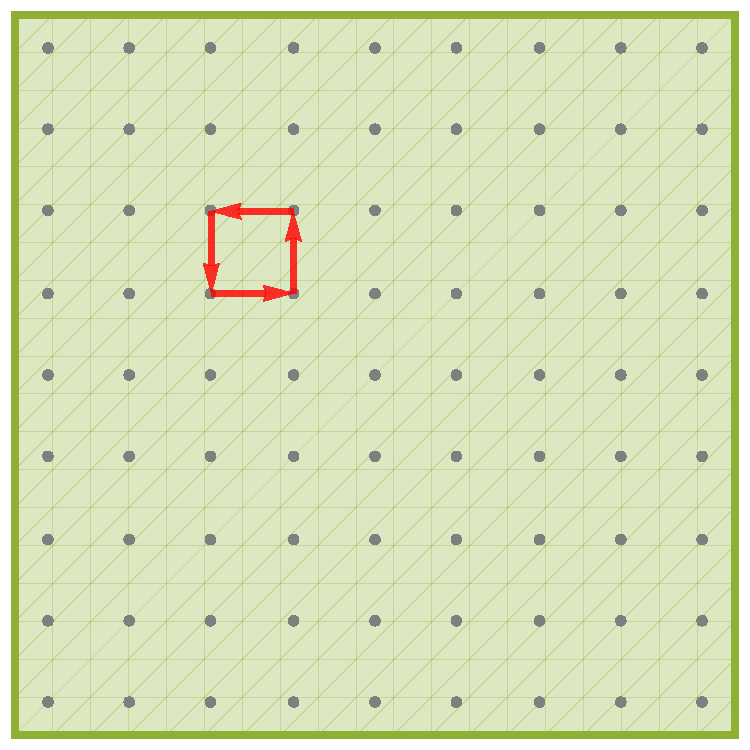
\includegraphics[width=0.5\columnwidth]{appendix/loop}
\caption{二维离散化参数空间中构造 Wilson 环路的示意图。数字标记环路中的顺序。}\label{fig:topoml-appendix}
\end{figure}

\begin{enumerate}

\item 计算每个边上相邻格点上波函数的内积,具体如下,引入
\begin{align}
U_{21} &= V^{\dagger}(\vect{k}_2) V(\vect{k}_1) \\ 
U_{32} &= V^{\dagger}(\vect{k}_3) V(\vect{k}_2) \\ 
U_{43} &= V^{\dagger}(\vect{k}_4) V(\vect{k}_3) \\ 
U_{14} &= V^{\dagger}(\vect{k}_1) V(\vect{k}_4) 
\end{align}

\item 定义 $\mathcal{U}_{ij} = \text{diag}(U_{ij})$,即取出矩阵$U_{ij}$的对角线元素构造对角矩阵,$(\mathcal{U}_{ij})_{mn}:=\delta_{mn}(U_{ij})_{nn}$。

\item 引入 $T_{\text{loop}}(\vect{k}_1) = \mathcal{U}_{14}\mathcal{U}_{43}\mathcal{U}_{32}\mathcal{U}_{21}$,则该由 $\vect{k}_1$ 所标记的方块上第 $n$ 个能带的 Berry 曲率 $\mathcal{F}_{xy}^{(n)}(\vect{k}_1)$ 被定义(计算)为:
\begin{align}
\theta(\vect{k}) = -i \log(T_{\text{loop}}(k_i, k_j))_{nn}\; ,
\qquad    
\mathcal{F}_{xy}^{(n)}(\vect{k}) = \theta(\vect{k}) / s(\vect{k})
\end{align}
$\theta$ 即所谓固体角。

\end{enumerate}

\item Chern 数即为所有方块上固体角之和。即,第 $n$ 个能带的 Chern 数 $c_n$ 由下式得到:

\begin{align}
c_n &= \frac{1}{2\pi} \sum_{i=1}^{L\times L} \theta(\vect{k}_i) \notag \\ 
&= \frac{1}{2\pi}\sum_{i=1}^{L}\sum_{j=1}^{L} -i \log T_{\text{loop}}^{(nn)}(k_i, k_j)
\end{align}

\end{enumerate}

以上即离散化 Chern 数的定义与算法。可以证明,这样定义/计算的 Chern 数具有量子化、规范不变的性质,且当离散化比较大时即能重现连续版本的 Chern 数值。




\begin{theorem}
上述算法计算的 Chern 数一定为整数。
\end{theorem}

\begin{proof}
考虑某一具体的能带,某一方块上 Wilson 环路四条边上两端的本征态的内积简记作 $\langle1|4\rangle$, $\langle4|3\rangle$, $\langle3|2\rangle$, $\langle2|1\rangle$,则
\begin{align}
\theta &= -i\log (\langle1|4\rangle\langle4|3\rangle\langle3|2\rangle\langle2|1\rangle) \\ 
&= (-i\log \langle1|4\rangle + -i\log \langle4|3\rangle + -i\log \langle3|2\rangle + -i\log \langle2|1\rangle) + 2m\pi
\end{align}
其中 $m$ 为某一整数。
而 Chern 数等于所有 plaquette 上这样的 $\theta$ 之和。注意到,每个 link 上会做两次内积且方向相反,也就是说,例如 $\langle3|2\rangle$ 和 $\langle2|3\rangle$ 各有一次。而这两者是互为共轭的,对于确定好的割线,这两个复数的相角是互为相反数的,也即,
\begin{align}
-i\log \langle3|2\rangle + -i\log\langle2|3\rangle = 0
\end{align}
其他 link 类似。因此,对最后计算出来的 Chern 数有
\begin{align}
c_n = \frac{1}{2\pi}\sum \theta = 0 + \frac{1}{2\pi}(2n\pi) = n
\end{align}
$n$ 为某一整数。证毕。
\end{proof}


\begin{theorem}
上述算法计算的 Chern 数与波函数所选取的规范无关。
\end{theorem}

\begin{proof}
对波函数做一个任意的规范变换,
\begin{align}
|u(\vect{k})\rangle \rightarrow |\tilde{u}(\vect{k})\rangle = e^{\ii\chi(\vect{k})}|u(\vect{k})\rangle
\end{align}
$\chi(\vect{k})$ 为一任意相位,则
\begin{align}
\tilde{T} 
&= \langle\tilde{u}(\vect{k}_1)|\tilde{u}(\vect{k}_4)\rangle\langle\tilde{u}(\vect{k}_4)|\tilde{u}(\vect{k}_3)\rangle\langle\tilde{u}(\vect{k}_3)|\tilde{u}(\vect{k}_2)\rangle\langle\tilde{u}(\vect{k}_2)|\tilde{u}(\vect{k}_1)\rangle \\
&= \langle u(\vect{k}_1)|u(\vect{k}_4)\rangle\langle u(\vect{k}_4)|u(\vect{k}_3)\rangle\langle u(\vect{k}_3)|u(\vect{k}_2)\rangle\langle u(\vect{k}_2)|u(\vect{k}_1)\rangle \nonumber\\
& \quad \times e^{\ii[\chi(\vect{k}_1)-\chi(\vect{k}_2)+\chi(\vect{k}_2)-\chi(\vect{k}_3)+\chi(\vect{k}_3)-\chi(\vect{k}_4)+\chi(\vect{k}_4)-\chi(\vect{k}_1)]} \\ 
&= \langle u(\vect{k}_1)|u(\vect{k}_4)\rangle\langle u(\vect{k}_4)|u(\vect{k}_3)\rangle\langle u(\vect{k}_3)|u(\vect{k}_2)\rangle\langle u(\vect{k}_2)|u(\vect{k}_1)\rangle \\
&= T
\end{align}
因此 $\tilde{\theta} = \theta$ 不变。Chern 数计算结果不变。
即该算法具有规范不变性。证毕。
\end{proof}

% \begin{proof}
% 容易验证,对任意 $\vect{k}$ 点处的波函数乘任意相角,牵涉到该点的 plaquette 上的 Berry 曲率不变。例如,
% \begin{align}
% |\tilde{3}\rangle = e^{i\chi} |3\rangle
% \end{align}
% 则
% \begin{align}
% \langle1|4\rangle\langle4|\tilde{3}\rangle\langle\tilde{3}|2\rangle\langle2|1\rangle 
% &= \langle1|4\rangle\langle4|e^{i\chi}|3\rangle\langle3|e^{-i\chi}|2\rangle\langle2|1\rangle \\
% &= \langle1|4\rangle\langle4|3\rangle\langle3|2\rangle\langle2|1\rangle
% \end{align}
% 即 $\tilde{\theta} = \theta$ 不变。因此,对任意 $\vect{k}$ 取任意规范 Chern 数计算结果不变。即该算法具有规范不变性。证毕。
% \end{proof}

\begin{theorem}
上述算法得到的 Berry 曲率,其离散化很大的极限($L\rightarrow\infty$,$\Delta k\rightarrow0$)等于连续版本的 Berry 曲率;对于没有很奇异的情况的模型,有限离散化的 Chern 数计算结果就可以完全准确地得到 连续的 Chern 数结果。
\end{theorem}

\begin{proof}
易验证\footnote{这里为简化记号,不致混淆的情况下以 $(x,y)$ 代记 $(k_x,k_y)$}:
\begin{align}
\langle u(\vect{k}_2)|u(\vect{k}_1)\rangle 
&= \langle u(x_{i+1},y_j)|u(x_i,y_j)\rangle \\ 
&= (\langle u(x_i,y_j)| + \Delta k_x\langle\partial_xu(x_i,y_j)|)|u(x_i,y_j)\rangle \\ 
&= 1 + \Delta k_x \langle\partial_xu(x_i,y_j)|u(x_i,y_j)\rangle \\ 
&= 1 - \Delta k_x \langle u(x_i,y_j)|\partial_xu(x_i,y_j)\rangle \\
&\rightarrow 1 + \ii \int_1^2A(x_i,y_j)d\vect{k}_x
\end{align}
因此有
\begin{align}
\lim_{\Delta k\rightarrow0} T_{\text{loop}}^{(nn)}(x_i,y_i) = 
1 + \ii \oint_{\square} \vect{A}(\vect{k})\cdot d\vect{k} = e^{\ii\theta(\vect{k}) S_{\square}} 
\end{align}
其中,$S_{\square}$ 为方块面积。$\theta(\vect{k})$ 即连续版本的 Berry 曲率。定理前半部分证毕。

定理后半部分:当没有“很”奇异的情况时\footnote{很奇异的情况,如 Berry curvature 发散},有限离散化即可完全准确重现(算出)连续版本的 Chern 数,这个有限离散化的下界 $L_0$ 由 Berry 场中最奇异(绝对值最大)的一点 $\theta_m$ 决定:
\begin{align}
\left(\dfrac{2\pi}{L_0}\right)^2 \sim \dfrac{\pi}{\theta_{m}}
\end{align}
$L$ 比 $L_0$ 大很多时即可认为算法完全有效(完全准确)。
\footnote{读者可以想一想为什么}
\end{proof}







注意,以上三个定理体现出该算法的强大性。比起连续版本下通过解析计算的复杂与极端情况下(如某处具有很奇异的 Berry 曲率时)的不准确,该算法不但简单,易算,速度快\footnote{经测试离散化到 $100\times100$ 时计算 Haldane 模型的 Chern 数只需 100毫秒的量级(python3, Mathematica)},而且准确,鲁棒。实际运行代码时,只有当遇到能隙关闭(gapless)的情况时可能会给出非整数的结果\footnote{对于这种情况,需要说明的是,上述定理1并未被违反,出现非整数的情况是由于实际计算中机器精度的问题。具体来说,当遇到能带简并的情况时,程序有可能在临近的某两个点对角化得到的波函数内积为0,或无限趋近于0,内积为0本身是没有问题的,但由于计算机机器精度的存在,可能会给存储的数本身附加上一个很小的实部和虚部,而这会引入任意的相角。理论上讲,一个有序的link上的内积和它的反向内积得到的数应互为共轭,但此时由于两者都被引入了任意相角,可能不再共轭,这就是会使最后算得的Chern数不为整数的来源。这个问题本身可以通过对程序做一些优化来避免。但仍需注意,gapless 情况本身就不应该计算 Chern 数。}——而这种情况本是不被允许计算 Chern 数的\footnote{能隙关闭的情况下,能隙关闭的点上能级是简并的,无法定义哪个态属于哪个能带\cite{topobook}。这样的情况也恰好是不同拓扑相相变的边界。}。


对于该 Chern 数算法,我们开发了专门的程序包,分别基于 python3 语言\footnote{python3 v3.7.2, package dependency: numpy}和 Wolfram Mathematica 语言\footnote{Mathematica v11.3}。开源地址\cite{repo-chern} https://github.com/atom-sun/chern。

% \newcommand{\vect}{\boldsymbol}
% \newcommand{\vect}{\mathbf}

\chapter{二维材料 Chern 数算法}\label{sec:chern}

考虑无限大二维材料的布里渊区(Brillioun Zone,简称BZ),其由两个实参数刻画,$\{k_x, k_y\}$,也即准动量$\vect{k}=(k_x, k_y)$。参数空间为 Torus 结构 (以下简称$T^2$),即 $k_x\in[0, 2\pi]$, $k_y\in[0, 2\pi]$,且 0 与 $2\pi$ 等价。考虑该材料的某一能带,引入其波函数记作 $|u(\vect{k})\rangle$,则陈数(以下称 Chern 数)刻画了一个从该 Brillioun 区($T^2$)上的到一个球面(以下简称$S^2$)的映射:

\begin{align}
T^2 \rightarrow S^2 : C = \frac{1}{2\pi}\int_{T^2}d^2\vect{k} F_{xy}(k)
\end{align}
其中被积式 $F_{xy}(\vect{k})$ 即 $\vect{k}$ 处的 Berry 曲率,
\begin{align}
F_{\mu\nu}(\vect{k})&=\partial_{\mu}A_{\nu} - \partial_{\nu}A_{\mu} \\ 
A_{\mu}(\vect{k})&=i\langle u(\vect{k})|\partial_{\mu}u(\vect{k})\rangle
\end{align}

以上是连续 BZ 下计算某能带的 Chern 数的表达式。人们喜欢用连续化的理论描述世界(例如量子场论),连续化的世界可偏、可导、可积,表达式简洁、优美,具有一切良好的性质。然而真实世界(或者说人们可测、可算的世界)往往是离散的。例如此处,当材料并非无限大时,或当需要对材料进行数值计算时,BZ 被离散化成有限的格点,相应的,我们需要引入离散 BZ 下的 Chern 数和 Berry 曲率的定义(算法)。这即是定义,也是算法,当离散化足够大时可以重现出连续化情况下的结果。

下面是离散化 Chern 数的定义与算法,基于 Takahiro Fukui 等人 2005 年的文章\inlinecite{chern2005}:

\begin{enumerate}

\item 将二维参数空间离散化为 $L\times L$ 个格点\footnote{此为简单起见。离散化成$L\times M$也没有问题},格点被标记为 $\vect{k}=(k_x, k_y)$。引入周期性边界条件($L+1$ 等同于 1)\footnote{严格地说,并不一定要 $H(k_x)=H(k_x+2\pi)$, $H(k_y)=H(k_y+2\pi)$, 只要参数空间的拓扑结构为 $T^2$ 即可。例如,实际计算 Haldane 模型的 Chern 数时,只需要在参数空间中取定蜂巢晶格的倒格子元胞即可,某种取法下 $H(k_x, k_y) = H(k_x + 2\pi, k_y + \pi)$。},则共有 $L\times L$ 个方块(plaquette)。对于均匀的离散化,每个方块的面积为 $s(\vect{k})=\Delta k_x\Delta k_y$,这里 $\Delta k_x$ 和 $\Delta k_y$ 分别是 $k_x$ 和 $k_y$ 方向相邻格点的距离。

\item 在每个格点 $\vect{k}=(k_x, k_y)$ 上,对角化 Hamiltonian:
\begin{align}
H(\vect{k}) = V(\vect{k})D(\vect{k})V^{\dagger}(\vect{k})
\end{align}
得到第 $n$ 个能带的本征态 $|u^{(n)}(\vect{k})\rangle$。其中,$D(\vect{k})$ 是一个对角矩阵,对角元是每个能带的能量本征值,$V(\vect{k})$ 的列向量是相应能带的本征态。

\item 对于每个方块上的4个顶点构造一个有序的 Wilson 环路,如图所示\ref{fig:topoml-appendix},并做如下操作和计算。
\begin{figure}
\centering
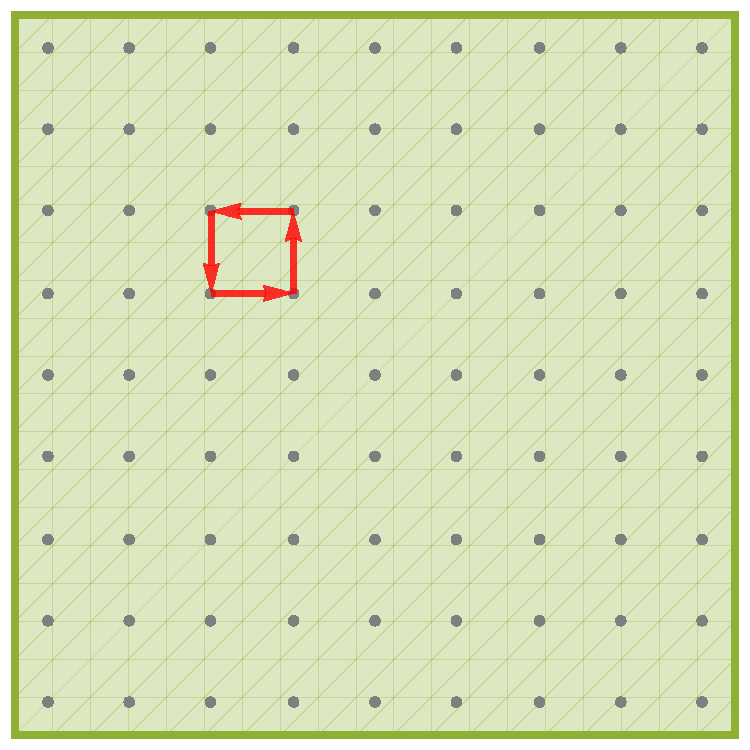
\includegraphics[width=0.5\columnwidth]{appendix/loop}
\caption{二维离散化参数空间中构造 Wilson 环路的示意图。数字标记环路中的顺序。}\label{fig:topoml-appendix}
\end{figure}

\begin{enumerate}

\item 计算每个边上相邻格点上波函数的内积,具体如下,引入
\begin{align}
U_{21} &= V^{\dagger}(\vect{k}_2) V(\vect{k}_1) \\ 
U_{32} &= V^{\dagger}(\vect{k}_3) V(\vect{k}_2) \\ 
U_{43} &= V^{\dagger}(\vect{k}_4) V(\vect{k}_3) \\ 
U_{14} &= V^{\dagger}(\vect{k}_1) V(\vect{k}_4) 
\end{align}

\item 定义 $\mathcal{U}_{ij} = \text{diag}(U_{ij})$,即取出矩阵$U_{ij}$的对角线元素构造对角矩阵,$(\mathcal{U}_{ij})_{mn}:=\delta_{mn}(U_{ij})_{nn}$。

\item 引入 $T_{\text{loop}}(\vect{k}_1) = \mathcal{U}_{14}\mathcal{U}_{43}\mathcal{U}_{32}\mathcal{U}_{21}$,则该由 $\vect{k}_1$ 所标记的方块上第 $n$ 个能带的 Berry 曲率 $\mathcal{F}_{xy}^{(n)}(\vect{k}_1)$ 被定义(计算)为:
\begin{align}
\theta(\vect{k}) = -i \log(T_{\text{loop}}(k_i, k_j))_{nn}\; ,
\qquad    
\mathcal{F}_{xy}^{(n)}(\vect{k}) = \theta(\vect{k}) / s(\vect{k})
\end{align}
$\theta$ 即所谓固体角。

\end{enumerate}

\item Chern 数即为所有方块上固体角之和。即,第 $n$ 个能带的 Chern 数 $c_n$ 由下式得到:

\begin{align}
c_n &= \frac{1}{2\pi} \sum_{i=1}^{L\times L} \theta(\vect{k}_i) \notag \\ 
&= \frac{1}{2\pi}\sum_{i=1}^{L}\sum_{j=1}^{L} -i \log T_{\text{loop}}^{(nn)}(k_i, k_j)
\end{align}

\end{enumerate}

以上即离散化 Chern 数的定义与算法。可以证明,这样定义/计算的 Chern 数具有量子化、规范不变的性质,且当离散化比较大时即能重现连续版本的 Chern 数值。




\begin{theorem}
上述算法计算的 Chern 数一定为整数。
\end{theorem}

\begin{proof}
考虑某一具体的能带,某一方块上 Wilson 环路四条边上两端的本征态的内积简记作 $\langle1|4\rangle$, $\langle4|3\rangle$, $\langle3|2\rangle$, $\langle2|1\rangle$,则
\begin{align}
\theta &= -i\log (\langle1|4\rangle\langle4|3\rangle\langle3|2\rangle\langle2|1\rangle) \\ 
&= (-i\log \langle1|4\rangle + -i\log \langle4|3\rangle + -i\log \langle3|2\rangle + -i\log \langle2|1\rangle) + 2m\pi
\end{align}
其中 $m$ 为某一整数。
而 Chern 数等于所有 plaquette 上这样的 $\theta$ 之和。注意到,每个 link 上会做两次内积且方向相反,也就是说,例如 $\langle3|2\rangle$ 和 $\langle2|3\rangle$ 各有一次。而这两者是互为共轭的,对于确定好的割线,这两个复数的相角是互为相反数的,也即,
\begin{align}
-i\log \langle3|2\rangle + -i\log\langle2|3\rangle = 0
\end{align}
其他 link 类似。因此,对最后计算出来的 Chern 数有
\begin{align}
c_n = \frac{1}{2\pi}\sum \theta = 0 + \frac{1}{2\pi}(2n\pi) = n
\end{align}
$n$ 为某一整数。证毕。
\end{proof}


\begin{theorem}
上述算法计算的 Chern 数与波函数所选取的规范无关。
\end{theorem}

\begin{proof}
对波函数做一个任意的规范变换,
\begin{align}
|u(\vect{k})\rangle \rightarrow |\tilde{u}(\vect{k})\rangle = e^{\ii\chi(\vect{k})}|u(\vect{k})\rangle
\end{align}
$\chi(\vect{k})$ 为一任意相位,则
\begin{align}
\tilde{T} 
&= \langle\tilde{u}(\vect{k}_1)|\tilde{u}(\vect{k}_4)\rangle\langle\tilde{u}(\vect{k}_4)|\tilde{u}(\vect{k}_3)\rangle\langle\tilde{u}(\vect{k}_3)|\tilde{u}(\vect{k}_2)\rangle\langle\tilde{u}(\vect{k}_2)|\tilde{u}(\vect{k}_1)\rangle \\
&= \langle u(\vect{k}_1)|u(\vect{k}_4)\rangle\langle u(\vect{k}_4)|u(\vect{k}_3)\rangle\langle u(\vect{k}_3)|u(\vect{k}_2)\rangle\langle u(\vect{k}_2)|u(\vect{k}_1)\rangle \nonumber\\
& \quad \times e^{\ii[\chi(\vect{k}_1)-\chi(\vect{k}_2)+\chi(\vect{k}_2)-\chi(\vect{k}_3)+\chi(\vect{k}_3)-\chi(\vect{k}_4)+\chi(\vect{k}_4)-\chi(\vect{k}_1)]} \\ 
&= \langle u(\vect{k}_1)|u(\vect{k}_4)\rangle\langle u(\vect{k}_4)|u(\vect{k}_3)\rangle\langle u(\vect{k}_3)|u(\vect{k}_2)\rangle\langle u(\vect{k}_2)|u(\vect{k}_1)\rangle \\
&= T
\end{align}
因此 $\tilde{\theta} = \theta$ 不变。Chern 数计算结果不变。
即该算法具有规范不变性。证毕。
\end{proof}

% \begin{proof}
% 容易验证,对任意 $\vect{k}$ 点处的波函数乘任意相角,牵涉到该点的 plaquette 上的 Berry 曲率不变。例如,
% \begin{align}
% |\tilde{3}\rangle = e^{i\chi} |3\rangle
% \end{align}
% 则
% \begin{align}
% \langle1|4\rangle\langle4|\tilde{3}\rangle\langle\tilde{3}|2\rangle\langle2|1\rangle 
% &= \langle1|4\rangle\langle4|e^{i\chi}|3\rangle\langle3|e^{-i\chi}|2\rangle\langle2|1\rangle \\
% &= \langle1|4\rangle\langle4|3\rangle\langle3|2\rangle\langle2|1\rangle
% \end{align}
% 即 $\tilde{\theta} = \theta$ 不变。因此,对任意 $\vect{k}$ 取任意规范 Chern 数计算结果不变。即该算法具有规范不变性。证毕。
% \end{proof}

\begin{theorem}
上述算法得到的 Berry 曲率,其离散化很大的极限($L\rightarrow\infty$,$\Delta k\rightarrow0$)等于连续版本的 Berry 曲率;对于没有很奇异的情况的模型,有限离散化的 Chern 数计算结果就可以完全准确地得到 连续的 Chern 数结果。
\end{theorem}

\begin{proof}
易验证\footnote{这里为简化记号,不致混淆的情况下以 $(x,y)$ 代记 $(k_x,k_y)$}:
\begin{align}
\langle u(\vect{k}_2)|u(\vect{k}_1)\rangle 
&= \langle u(x_{i+1},y_j)|u(x_i,y_j)\rangle \\ 
&= (\langle u(x_i,y_j)| + \Delta k_x\langle\partial_xu(x_i,y_j)|)|u(x_i,y_j)\rangle \\ 
&= 1 + \Delta k_x \langle\partial_xu(x_i,y_j)|u(x_i,y_j)\rangle \\ 
&= 1 - \Delta k_x \langle u(x_i,y_j)|\partial_xu(x_i,y_j)\rangle \\
&\rightarrow 1 + \ii \int_1^2A(x_i,y_j)d\vect{k}_x
\end{align}
因此有
\begin{align}
\lim_{\Delta k\rightarrow0} T_{\text{loop}}^{(nn)}(x_i,y_i) = 
1 + \ii \oint_{\square} \vect{A}(\vect{k})\cdot d\vect{k} = e^{\ii\theta(\vect{k}) S_{\square}} 
\end{align}
其中,$S_{\square}$ 为方块面积。$\theta(\vect{k})$ 即连续版本的 Berry 曲率。定理前半部分证毕。

定理后半部分:当没有“很”奇异的情况时\footnote{很奇异的情况,如 Berry curvature 发散},有限离散化即可完全准确重现(算出)连续版本的 Chern 数,这个有限离散化的下界 $L_0$ 由 Berry 场中最奇异(绝对值最大)的一点 $\theta_m$ 决定:
\begin{align}
\left(\dfrac{2\pi}{L_0}\right)^2 \sim \dfrac{\pi}{\theta_{m}}
\end{align}
$L$ 比 $L_0$ 大很多时即可认为算法完全有效(完全准确)。
\footnote{读者可以想一想为什么}
\end{proof}







注意,以上三个定理体现出该算法的强大性。比起连续版本下通过解析计算的复杂与极端情况下(如某处具有很奇异的 Berry 曲率时)的不准确,该算法不但简单,易算,速度快\footnote{经测试离散化到 $100\times100$ 时计算 Haldane 模型的 Chern 数只需 100毫秒的量级(python3, Mathematica)},而且准确,鲁棒。实际运行代码时,只有当遇到能隙关闭(gapless)的情况时可能会给出非整数的结果\footnote{对于这种情况,需要说明的是,上述定理1并未被违反,出现非整数的情况是由于实际计算中机器精度的问题。具体来说,当遇到能带简并的情况时,程序有可能在临近的某两个点对角化得到的波函数内积为0,或无限趋近于0,内积为0本身是没有问题的,但由于计算机机器精度的存在,可能会给存储的数本身附加上一个很小的实部和虚部,而这会引入任意的相角。理论上讲,一个有序的link上的内积和它的反向内积得到的数应互为共轭,但此时由于两者都被引入了任意相角,可能不再共轭,这就是会使最后算得的Chern数不为整数的来源。这个问题本身可以通过对程序做一些优化来避免。但仍需注意,gapless 情况本身就不应该计算 Chern 数。}——而这种情况本是不被允许计算 Chern 数的\footnote{能隙关闭的情况下,能隙关闭的点上能级是简并的,无法定义哪个态属于哪个能带\cite{topobook}。这样的情况也恰好是不同拓扑相相变的边界。}。


对于该 Chern 数算法,我们开发了专门的程序包,分别基于 python3 语言\footnote{python3 v3.7.2, package dependency: numpy}和 Wolfram Mathematica 语言\footnote{Mathematica v11.3}。开源地址\cite{repo-chern} https://github.com/atom-sun/chern。

\end{appendix}

%% 致谢
% % 如果使用声明扫描页,将可选参数指定为扫描后的 PDF 文件名,例如:
% \begin{acknowledgement}[scan-statement.pdf]
\begin{acknowledgement}

首先,我要感谢我的导师翟荟教授,他的悉心指导使我在这四年的读博历程中收获巨大,
不枉此行。翟荟教授指导我深入冷原子这个方兴未艾的领域进行研究,在光晶格体系的拓
扑和动力学性质方面做出成果,后来又把我引导到机器学习这个生气蓬勃的领域,使我对
新兴领域保持开放心态。翟荟教授扎实、务实的研究风格,认真、细致的研究态度,和与
实验相结合、追求简单而普适的美的研究品味使我深受影响。而他在做人做事方面的言传
身教,更是让我学到数不尽的东西。我很幸运能有这样一位导师,而且不仅是一位学术上
的导师,更是我未来人生道路上的榜样和参考。

感谢林励庆教授,尤其是在我接触科研初期他的耐心指导和无私帮助。他在科研工作上的
认真细致、精益求精,和对于生活的有品位的追求都影响到了我。
感谢余金龙博士、张鹏飞、易近民、沈汇涛等同学,他们勤奋靠谱,和他们的合作十分愉快。
感谢崔晓玲老师、郑炜博士等许多老师和同学们,和他们的讨论给我许多启发。
感谢叶柄天同学曾经给予我的许多帮助和支持。
% 感谢何天伦教授、崔晓玲教授、易为教授、张威教授、张芃教授、王磊研究员等许多老师,
% 易为教授、张芃教授、张威教授、曾蓓教授、尤亦庄教授、吴志钢教授等老师
% 和吴志钢博士、王策、吴亚东等许多同学,和他们的讨论给我许多启发。
感谢中国人民大学的李涛教授,是他的推荐使我得以有此科研经历,他的扎实的理论功底
和对物理学研究的纯粹的热情使我深受感染。
此外,感谢李凌博士及其团队,和他们一起工作的经历愉快而难忘。
感谢李凌博士在编程方面对我的训练和指导。
感谢吴限学长在许多方面对我的慷慨帮助。
% 另外,
感谢文昊旻博士在数学方面的有益讨论。
感谢 ThuThesis 模版对我论文写作的助益。
感谢 @PP猪的日常,他们的创作为我的生活带来许多欢乐。

最后,我要再次感谢我的老伴儿张鹏飞,感谢他日常的陪伴与支持。
% 也特别感谢他在我完成此论文过程中的帮助。
他教过我场论,也教我玩电子游戏;他在我干活停不下来的时候让我及时停下来休息,
也在我一拖再拖的时候日夜督促我完成此篇论文。
% 我们讨论过很多问题,这些讨论帮助我理解了许多事情。
他是我见过的同龄人中最懂得实事求是、知行合一的人。
我很幸运能在这里遇到他、认识他,这是我读博4年最大的收获。

% 最后,再次感谢张鹏飞同学一直以来的陪伴,以及在我完成毕业论文期间的巨大帮助。

\end{acknowledgement}

% 如果使用声明扫描页,将可选参数指定为扫描后的 PDF 文件名,例如:
% \begin{acknowledgement}[scan-statement.pdf]
\begin{acknowledgement}

首先,我要感谢我的导师翟荟教授,他的悉心指导使我在这四年的读博历程中收获巨大,
不枉此行。翟荟教授指导我深入冷原子这个方兴未艾的领域进行研究,在光晶格体系的拓
扑和动力学性质方面做出成果,后来又把我引导到机器学习这个生气蓬勃的领域,使我对
新兴领域保持开放心态。翟荟教授扎实、务实的研究风格,认真、细致的研究态度,和与
实验相结合、追求简单而普适的美的研究品味使我深受影响。而他在做人做事方面的言传
身教,更是让我学到数不尽的东西。我很幸运能有这样一位导师,而且不仅是一位学术上
的导师,更是我未来人生道路上的榜样和参考。

感谢林励庆教授,尤其是在我接触科研初期他的耐心指导和无私帮助。他在科研工作上的
认真细致、精益求精,和对于生活的有品位的追求都影响到了我。
感谢余金龙博士、张鹏飞、易近民、沈汇涛等同学,他们勤奋靠谱,和他们的合作十分愉快。
感谢崔晓玲老师、郑炜博士等许多老师和同学们,和他们的讨论给我许多启发。
感谢叶柄天同学曾经给予我的许多帮助和支持。
% 感谢何天伦教授、崔晓玲教授、易为教授、张威教授、张芃教授、王磊研究员等许多老师,
% 易为教授、张芃教授、张威教授、曾蓓教授、尤亦庄教授、吴志钢教授等老师
% 和吴志钢博士、王策、吴亚东等许多同学,和他们的讨论给我许多启发。
感谢中国人民大学的李涛教授,是他的推荐使我得以有此科研经历,他的扎实的理论功底
和对物理学研究的纯粹的热情使我深受感染。
此外,感谢李凌博士及其团队,和他们一起工作的经历愉快而难忘。
感谢李凌博士在编程方面对我的训练和指导。
感谢吴限学长在许多方面对我的慷慨帮助。
% 另外,
感谢文昊旻博士在数学方面的有益讨论。
感谢 ThuThesis 模版对我论文写作的助益。
感谢 @PP猪的日常,他们的创作为我的生活带来许多欢乐。

最后,我要再次感谢我的老伴儿张鹏飞,感谢他日常的陪伴与支持。
% 也特别感谢他在我完成此论文过程中的帮助。
他教过我场论,也教我玩电子游戏;他在我干活停不下来的时候让我及时停下来休息,
也在我一拖再拖的时候日夜督促我完成此篇论文。
% 我们讨论过很多问题,这些讨论帮助我理解了许多事情。
他是我见过的同龄人中最懂得实事求是、知行合一的人。
我很幸运能在这里遇到他、认识他,这是我读博4年最大的收获。

% 最后,再次感谢张鹏飞同学一直以来的陪伴,以及在我完成毕业论文期间的巨大帮助。

\end{acknowledgement}


%% 个人简历
% \begin{resume}

    \resumeitem{个人简历}

    1993 年 5 月 10 日出生于 山东 省 淄博 市。
    2011 年 9 月考入中国人民大学物理系物理学专业,2015 年 7 月本科毕业并获得
    理学学士学位。
    2015 年 8 月免试进入 清华大学 大学 高等研究 院攻读 物理学博士 学位至今。

    \researchitem{发表的学术论文} % 发表的和录用的合在一起

    % 1. 已经刊载的学术论文(本人是第一作者,或者导师为第一作者本人是第二作者)
    \begin{publications}
        \item \textbf{Sun N}, Lim L K. Quantum charge pumps with topological phases in 
            a Creutz ladder. Physical Review B, 2017, 96(3): 035139.
        \item \textbf{Sun N}, Yi J, Zhang P, et al. Deep learning topological invariants 
            of band insulators. Physical Review B, 2018, 98(8): 085402.
        \item Zhai H, \textbf{Sun N}, Yu J, et al. New relations between spin and charge 
            dynamics of the Fermi Hubbard model. New Journal of Physics, 
            2018.
        \item \textbf{Sun N}, Zhang P, Zhai H. Resonant-driving-induced ferromagnetism in the Fermi-Hubbard model. Physical Review A, 2019, 99(4): 043629.
    \end{publications}
    ~

    % 2. 尚未刊载,但已经接到正式录用函的学术论文(本人为第一作者,或者
    %    导师为第一作者本人是第二作者)。
    % \begin{publications}[before=\publicationskip,after=\publicationskip]
    %     \item Sun N, Zhang P, Zhai H. Resonant driving induced ferromagnetism 
    %         in the Fermi Hubbard model. In press. (已被 录用. SCI 源刊.)
    % \end{publications}

    % 3. 其他学术论文。可列出除上述两种情况以外的其他学术论文,但必须是
    %    已经刊载或者收到正式录用函的论文。
    \begin{publications}
        \item Yu J, \textbf{Sun N}, Zhai H. Symmetry Protected Dynamical Symmetry in 
        the Generalized Hubbard Models. Physical Review Letters, 2017, 119(22): 225302.
        \item Zhang P, \textbf{Sun N}. Universal relations for spin-orbit-coupled 
        Fermi gas near an s-wave resonance. Physical Review A, 2018, 97(4): 040701.
    \end{publications}

\end{resume}

\begin{resume}

    \resumeitem{个人简历}

    1993 年 5 月 10 日出生于 山东 省 淄博 市。
    2011 年 9 月考入中国人民大学物理系物理学专业,2015 年 7 月本科毕业并获得
    理学学士学位。
    2015 年 8 月免试进入 清华大学 大学 高等研究 院攻读 物理学博士 学位至今。

    \researchitem{发表的学术论文} % 发表的和录用的合在一起

    % 1. 已经刊载的学术论文(本人是第一作者,或者导师为第一作者本人是第二作者)
    \begin{publications}
        \item \textbf{Sun N}, Lim L K. Quantum charge pumps with topological phases in 
            a Creutz ladder. Physical Review B, 2017, 96(3): 035139.
        \item \textbf{Sun N}, Yi J, Zhang P, et al. Deep learning topological invariants 
            of band insulators. Physical Review B, 2018, 98(8): 085402.
        \item Zhai H, \textbf{Sun N}, Yu J, et al. New relations between spin and charge 
            dynamics of the Fermi Hubbard model. New Journal of Physics, 
            2018.
        \item \textbf{Sun N}, Zhang P, Zhai H. Resonant-driving-induced ferromagnetism in the Fermi-Hubbard model. Physical Review A, 2019, 99(4): 043629.
    \end{publications}
    ~

    % 2. 尚未刊载,但已经接到正式录用函的学术论文(本人为第一作者,或者
    %    导师为第一作者本人是第二作者)。
    % \begin{publications}[before=\publicationskip,after=\publicationskip]
    %     \item Sun N, Zhang P, Zhai H. Resonant driving induced ferromagnetism 
    %         in the Fermi Hubbard model. In press. (已被 录用. SCI 源刊.)
    % \end{publications}

    % 3. 其他学术论文。可列出除上述两种情况以外的其他学术论文,但必须是
    %    已经刊载或者收到正式录用函的论文。
    \begin{publications}
        \item Yu J, \textbf{Sun N}, Zhai H. Symmetry Protected Dynamical Symmetry in 
        the Generalized Hubbard Models. Physical Review Letters, 2017, 119(22): 225302.
        \item Zhang P, \textbf{Sun N}. Universal relations for spin-orbit-coupled 
        Fermi gas near an s-wave resonance. Physical Review A, 2018, 97(4): 040701.
    \end{publications}

\end{resume}


%% 本科生进行格式审查是需要下面这个表格,答辩可能不需要。选择性留下。
% 综合论文训练记录表
% 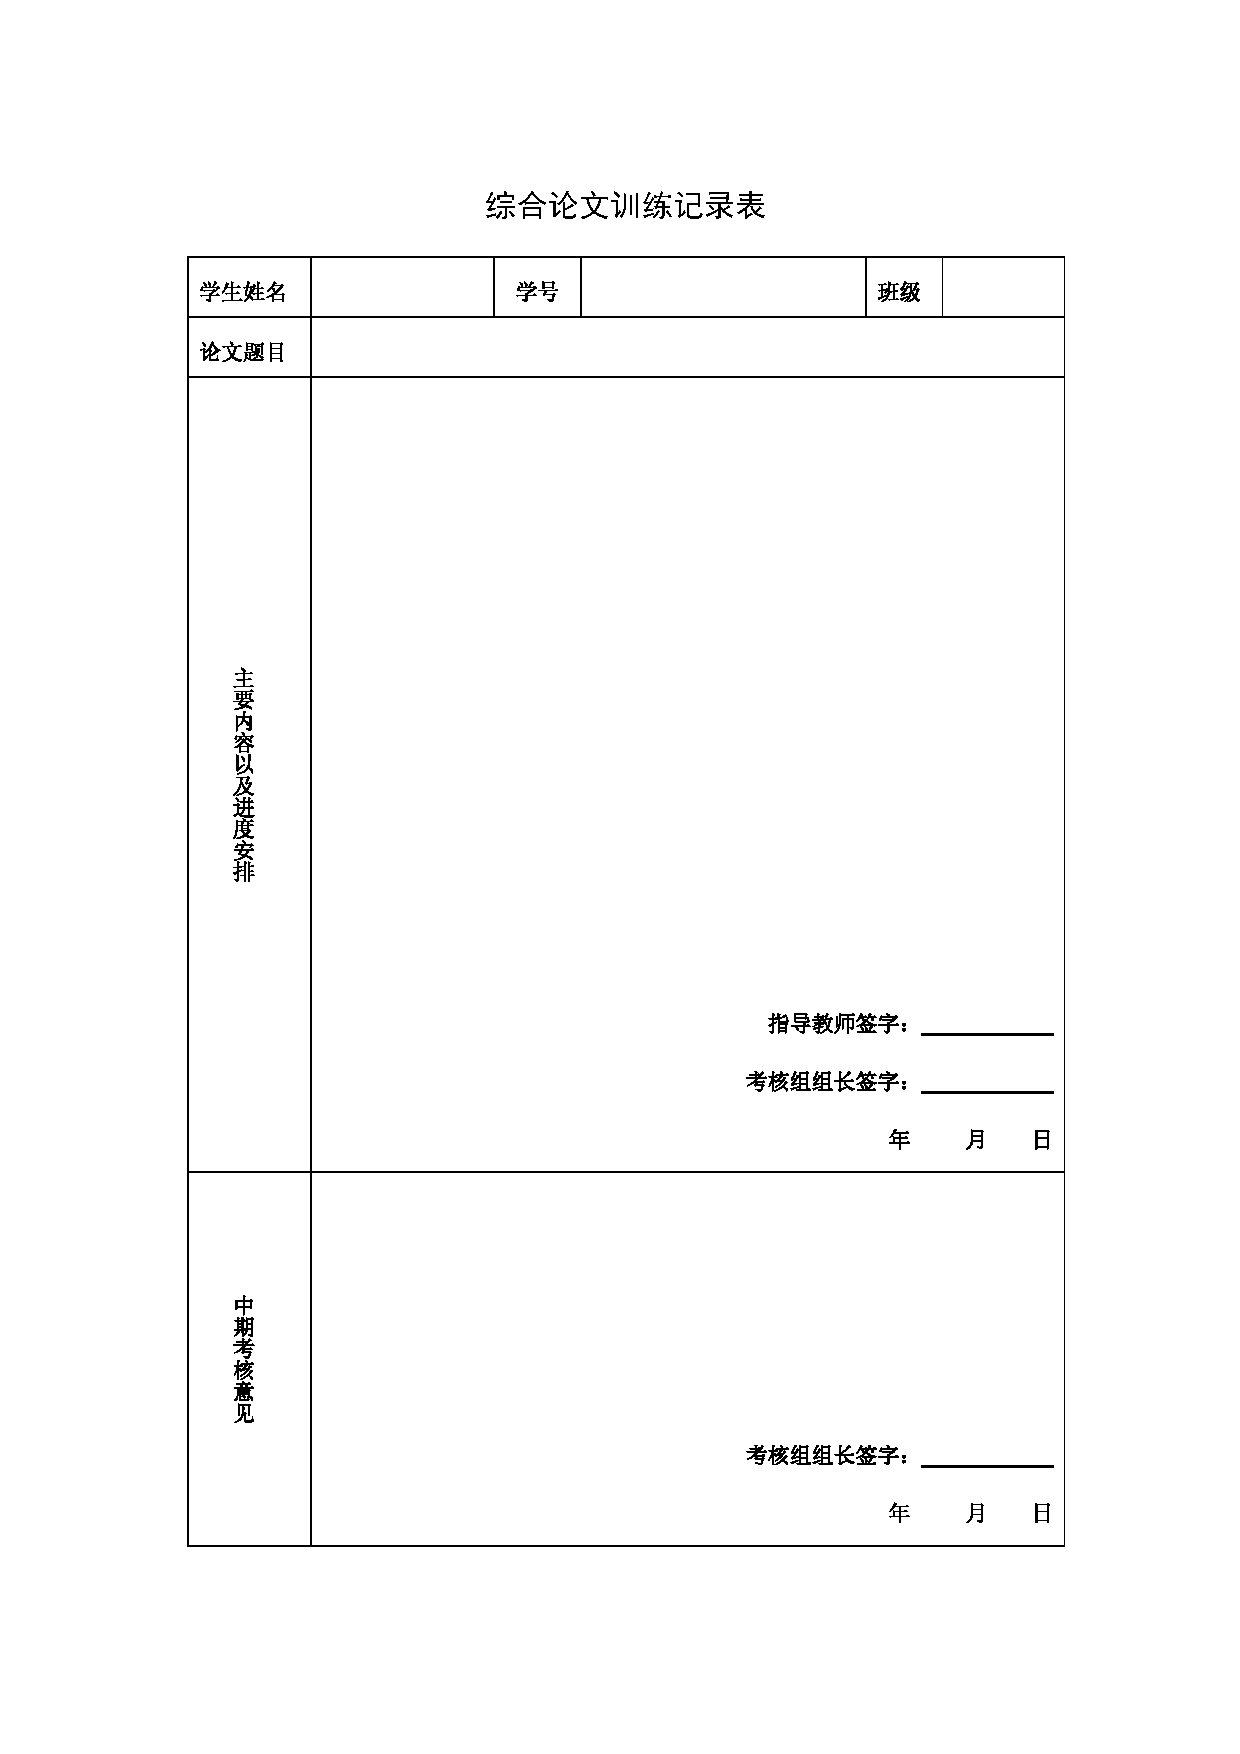
\includepdf[pages=-]{scan-record.pdf}
\end{document}
